\documentclass[10pt,aspectratio=43]{beamer}

% =========================================================================
% Governing Equations of Fluid Flow with Chemistry
% Prof. Dr. Onur Tuncer -- Istanbul Technical University
% Beamer source converted from the original PowerPoint deck.
% =========================================================================

\usetheme{Madrid}
\usecolortheme{seahorse}
\useinnertheme{rectangles}
\useoutertheme{infolines}

\setbeamertemplate{navigation symbols}{}
\setbeamerfont{frametitle}{size=\normalsize,series=\bfseries}
\setbeamerfont{title}{size=\large,series=\bfseries}

\usepackage[T1]{fontenc}
\usepackage[utf8]{inputenc}
\usepackage{amsmath,amssymb,amsfonts,mathtools}
\usepackage{bm}
\usepackage{graphicx}
\usepackage{booktabs}
\usepackage{array}
\usepackage{xcolor}
\usepackage{caption}
\captionsetup[figure]{font=footnotesize,labelformat=empty}

\graphicspath{{fig/}}

% --- shorthands -----------------------------------------------------------
\newcommand{\dd}{\mathrm{d}}
\newcommand{\D}{\mathrm{D}}
\newcommand{\Dt}{\frac{\D}{\D t}}
\newcommand{\pd}[2]{\frac{\partial #1}{\partial #2}}
\newcommand{\bu}{\mathbf{u}}
\newcommand{\bF}{\mathbf{F}}
\newcommand{\bx}{\mathbf{x}}
\newcommand{\bn}{\mathbf{n}}
\newcommand{\bg}{\mathbf{g}}
\newcommand{\divg}{\nabla\!\cdot}
\newcommand{\Vol}{\mathcal{V}}
\renewcommand{\div}{\nabla\!\cdot}

\title[Fluid Flow with Chemistry]{Governing Equations of Fluid Flow with Chemistry}
\author[O. Tun\c{c}er]{Prof.\ Dr.\ Onur Tun\c{c}er}
\institute[ITU]{Istanbul Technical University \\ Department of Aeronautical Engineering}
\date{March 5, 2026}

\begin{document}

% =========================================================================
% Slide 1 -- Title
% =========================================================================
\begin{frame}[plain]
  \titlepage
  \begin{center}
    
\includegraphics[height=1.6cm]{itu_logo.png}
  \end{center}
\end{frame}

% =========================================================================
% Slide 2 -- Definition of a Fluid
% =========================================================================
\begin{frame}{Definition of a Fluid}
  A \alert{fluid} is a substance that continually deforms (flows) under an
  applied shear stress, no matter how small.

  \medskip
  Fluids display such properties as:
  \begin{itemize}
    \item not resisting deformation, or resisting it only lightly (\emph{viscosity});
    \item the ability to flow (also described as the ability to take on the
          shape of the container)\,---\,all fluids therefore have the property
          of \emph{fluidity}.
  \end{itemize}

  \medskip
  These properties are typically a function of their inability to support a
  shear stress in static equilibrium.
\end{frame}

% =========================================================================
% Slide 3 -- Knudsen Number
% =========================================================================
\begin{frame}{Knudsen Number and Continuum Concept}
  The Knudsen number $Kn$ is a dimensionless number defined as the ratio of
  the molecular mean free path length to a representative physical length
  scale. Named after the Danish physicist Martin Knudsen (1871--1949).
  \[
    Kn \;=\; \frac{\lambda}{L}
  \]
  \begin{tabular}{rl}
    $\lambda$ & molecular mean free path length \\
    $L$       & representative physical length scale
  \end{tabular}

  For an ideal gas,
  \[
    Kn \;=\; \frac{k_{B}\,T}{\sqrt{2}\,\sigma^{2}\,p\,L}
  \]
  with $k_{B}$ Boltzmann constant, $T$ thermodynamic temperature, $\sigma$
  particle hard-shell diameter, $p$ total pressure. At STP for atmospheric
  particles ($25^{\circ}$C, $1$~atm) one finds $\lambda \approx 8\times 10^{-8}$~m.
\end{frame}

% =========================================================================
% Slide 4 -- Continuity Assumption
% =========================================================================
\begin{frame}{The Continuity Assumption}
  The continuity assumption considers fluids to be \alert{continuous}: properties
  such as density, pressure, temperature and velocity are taken to be
  well-defined at infinitely small points and are assumed to vary continuously
  from one point to another.

  \medskip
  The discrete, molecular nature of a fluid is ignored.

  \medskip
  \begin{columns}[t]
    \column{0.5\textwidth}
    \begin{itemize}
      \item Density \quad $\rho(\bx,t)$
      \item Velocity \quad $\bu(\bx,t)$
    \end{itemize}
    \column{0.5\textwidth}
    \begin{itemize}
      \item Pressure \quad $p(\bx,t)$
      \item Temperature \quad $T(\bx,t)$
    \end{itemize}
  \end{columns}
\end{frame}

% =========================================================================
% Slide 5 -- Microflows (image)
% =========================================================================
\begin{frame}{Cases Where the Continuum Assumption Fails (Microflows)}
  \begin{center}
    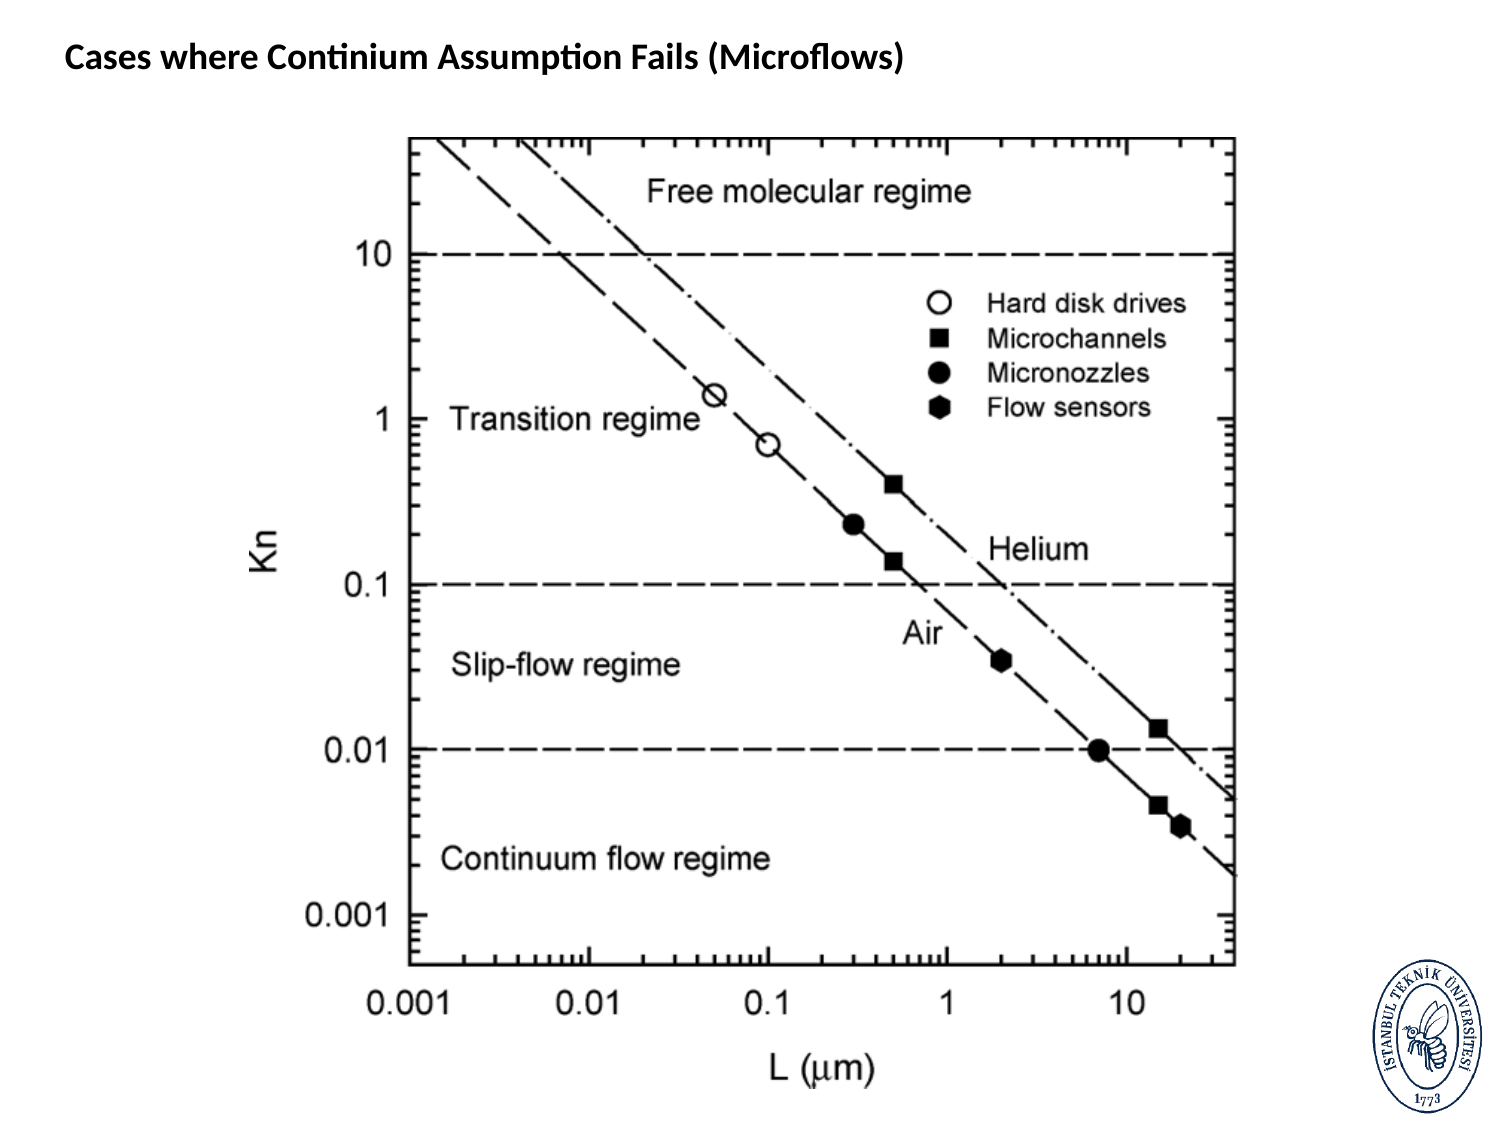
\includegraphics[width=0.85\linewidth,trim=10 40 10 40,clip]{slide5.png}
  \end{center}
\end{frame}

% =========================================================================
% Slide 6 -- Reentry (image)
% =========================================================================
\begin{frame}{Cases Where the Continuum Assumption Fails (Atmospheric Reentry)}
  \begin{center}
    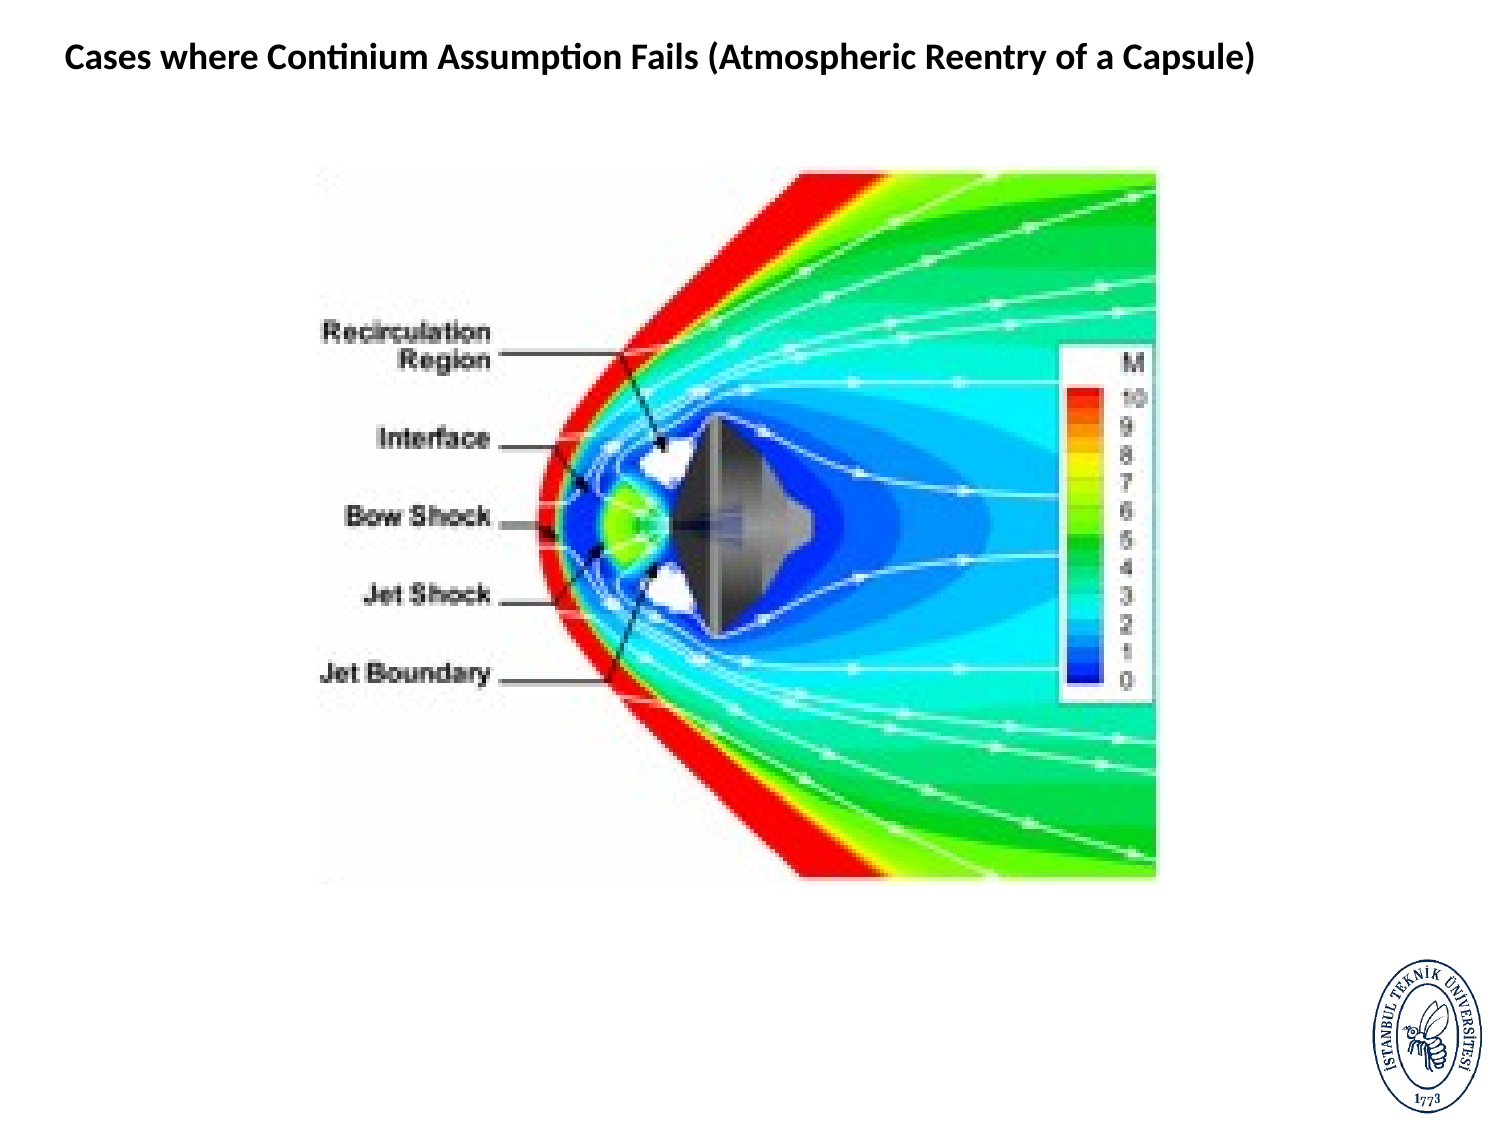
\includegraphics[width=0.85\linewidth,trim=10 40 10 40,clip]{slide6.png}
  \end{center}
\end{frame}

% =========================================================================
% Slide 7 -- Conservation Laws
% =========================================================================
\begin{frame}{Conservation Laws}
  Fluid flows obey conservation laws for \alert{mass}, \alert{momentum} and
  \alert{energy}.
  \begin{itemize}
    \item These laws can be stated in \emph{differential} form, applicable at
          a point.
    \item They can also be stated in \emph{integral} form, applicable to an
          extended region.
  \end{itemize}
\end{frame}

% =========================================================================
% Slide 8 -- Lagrangian / Eulerian
% =========================================================================
\begin{frame}{Two Different Ways of Observing Fluid Motion}
  \begin{block}{Lagrangian specification}
    A way of looking at fluid motion where the observer follows an individual
    fluid parcel as it moves through space and time (\emph{material volume}).
  \end{block}
  \begin{block}{Eulerian specification}
    A way of looking at fluid motion that focuses on specific locations in
    the space through which the fluid flows as time passes (\emph{control
    volume}).
  \end{block}
\end{frame}

% =========================================================================
% Slide 9 -- Material derivative
% =========================================================================
\begin{frame}{Material (Substantial) Derivative}
  The Lagrangian and Eulerian specifications of the kinematics and dynamics
  of the flow field are related by the \alert{substantial derivative} (also
  called the Lagrangian, convective, material, or particle derivative):
  \[
    \boxed{\;\frac{\D \bF}{\D t} \;=\; \pd{\bF}{t} \;+\; (\bu\!\cdot\!\nabla)\,\bF\;}
  \]
  The total rate of change of a vector function $\bF$, as a fluid parcel
  moves through a flow field described by its Eulerian specification $\bu$,
  equals the sum of the \emph{local} rate of change and the \emph{convective}
  rate of change of $\bF$.
\end{frame}

% =========================================================================
% Slide 10 -- Cartesian acceleration
% =========================================================================
\begin{frame}{Motion of a Fluid Particle (Kinematics)}
  \framesubtitle{Fluid translation: acceleration in a velocity field (Cartesian)}
  \begin{align*}
    a_{x_p} &= \frac{\D u}{\D t}
            = u\,\pd{u}{x} + v\,\pd{u}{y} + w\,\pd{u}{z} + \pd{u}{t} \\[2pt]
    a_{y_p} &= \frac{\D v}{\D t}
            = u\,\pd{v}{x} + v\,\pd{v}{y} + w\,\pd{v}{z} + \pd{v}{t} \\[2pt]
    a_{z_p} &= \frac{\D w}{\D t}
            = u\,\pd{w}{x} + v\,\pd{w}{y} + w\,\pd{w}{z} + \pd{w}{t}
  \end{align*}
\end{frame}

% =========================================================================
% Slide 11 -- Cylindrical acceleration
% =========================================================================
\begin{frame}{Motion of a Fluid Particle (Kinematics)}
  \framesubtitle{Fluid translation: acceleration in a velocity field (Cylindrical)}
  \begin{align*}
    a_{r_p}    &= V_{r}\,\pd{V_r}{r}
                  + \frac{V_\theta}{r}\,\pd{V_r}{\theta}
                  - \frac{V_\theta^{2}}{r}
                  + V_z\,\pd{V_r}{z}
                  + \pd{V_r}{t} \\[2pt]
    a_{\theta_p} &= V_{r}\,\pd{V_\theta}{r}
                  + \frac{V_\theta}{r}\,\pd{V_\theta}{\theta}
                  + \frac{V_r V_\theta}{r}
                  + V_z\,\pd{V_\theta}{z}
                  + \pd{V_\theta}{t} \\[2pt]
    a_{z_p}    &= V_{r}\,\pd{V_z}{r}
                  + \frac{V_\theta}{r}\,\pd{V_z}{\theta}
                  + V_z\,\pd{V_z}{z}
                  + \pd{V_z}{t}
  \end{align*}
\end{frame}

% =========================================================================
% Slide 12 -- Divergence Theorem
% =========================================================================
\begin{frame}{Divergence Theorem}
  The integral and differential forms can be derived from each other. During
  the derivation, surface integrals frequently need to be converted to
  volume integrals (or vice versa) by means of the Gauss divergence theorem:
  \[
    \int_{\Vol}\!\pd{F}{x_i}\,\dd\Vol \;=\; \int_{A}\! F\,\dd A_{i}
  \]
  where $F(\bx,t)$ is a tensor of any rank (including vectors and scalars),
  $\Vol$ is either a fixed volume or a material volume, and $A$ is its
  boundary surface.
\end{frame}

% =========================================================================
% Slide 13 -- Time derivatives of volume integrals
% =========================================================================
\begin{frame}{Time Derivatives of Volume Integrals}
  In deriving conservation laws one frequently faces the problem of finding
  the time derivative of integrals such as
  \[
    \frac{\dd}{\dd t}\int_{\Vol(t)} F\,\dd\Vol
  \]
  where $F(\bx,t)$ is a tensor of any order and $\Vol(t)$ is any region which
  may be fixed or moving with the fluid.
\end{frame}

% =========================================================================
% Slide 14 -- Leibnitz theorem
% =========================================================================
\begin{frame}{Leibnitz Theorem}
  Consider the general case when $\Vol(t)$ is neither a fixed volume nor a
  material volume\,---\,the surfaces of $\Vol$ are moving but not with the
  local fluid velocity. The rule for differentiating an integral becomes
  clear from a one-dimensional analogy:
  \[
    \boxed{\;\frac{\dd}{\dd t}\!\int_{x=a(t)}^{b(t)}\!F(x,t)\,\dd x
        \;=\; \int_{a}^{b}\!\pd{F}{t}\,\dd x
        \;+\; \frac{\dd b}{\dd t}\,F(b,t)
        \;-\; \frac{\dd a}{\dd t}\,F(a,t)\;}
  \]
  This is known as the \alert{Leibnitz theorem}.
\end{frame}

% =========================================================================
% Slide 15 -- Sketch of moving control volume
% =========================================================================
\begin{frame}{General Moving Control Volume}
  \begin{center}
    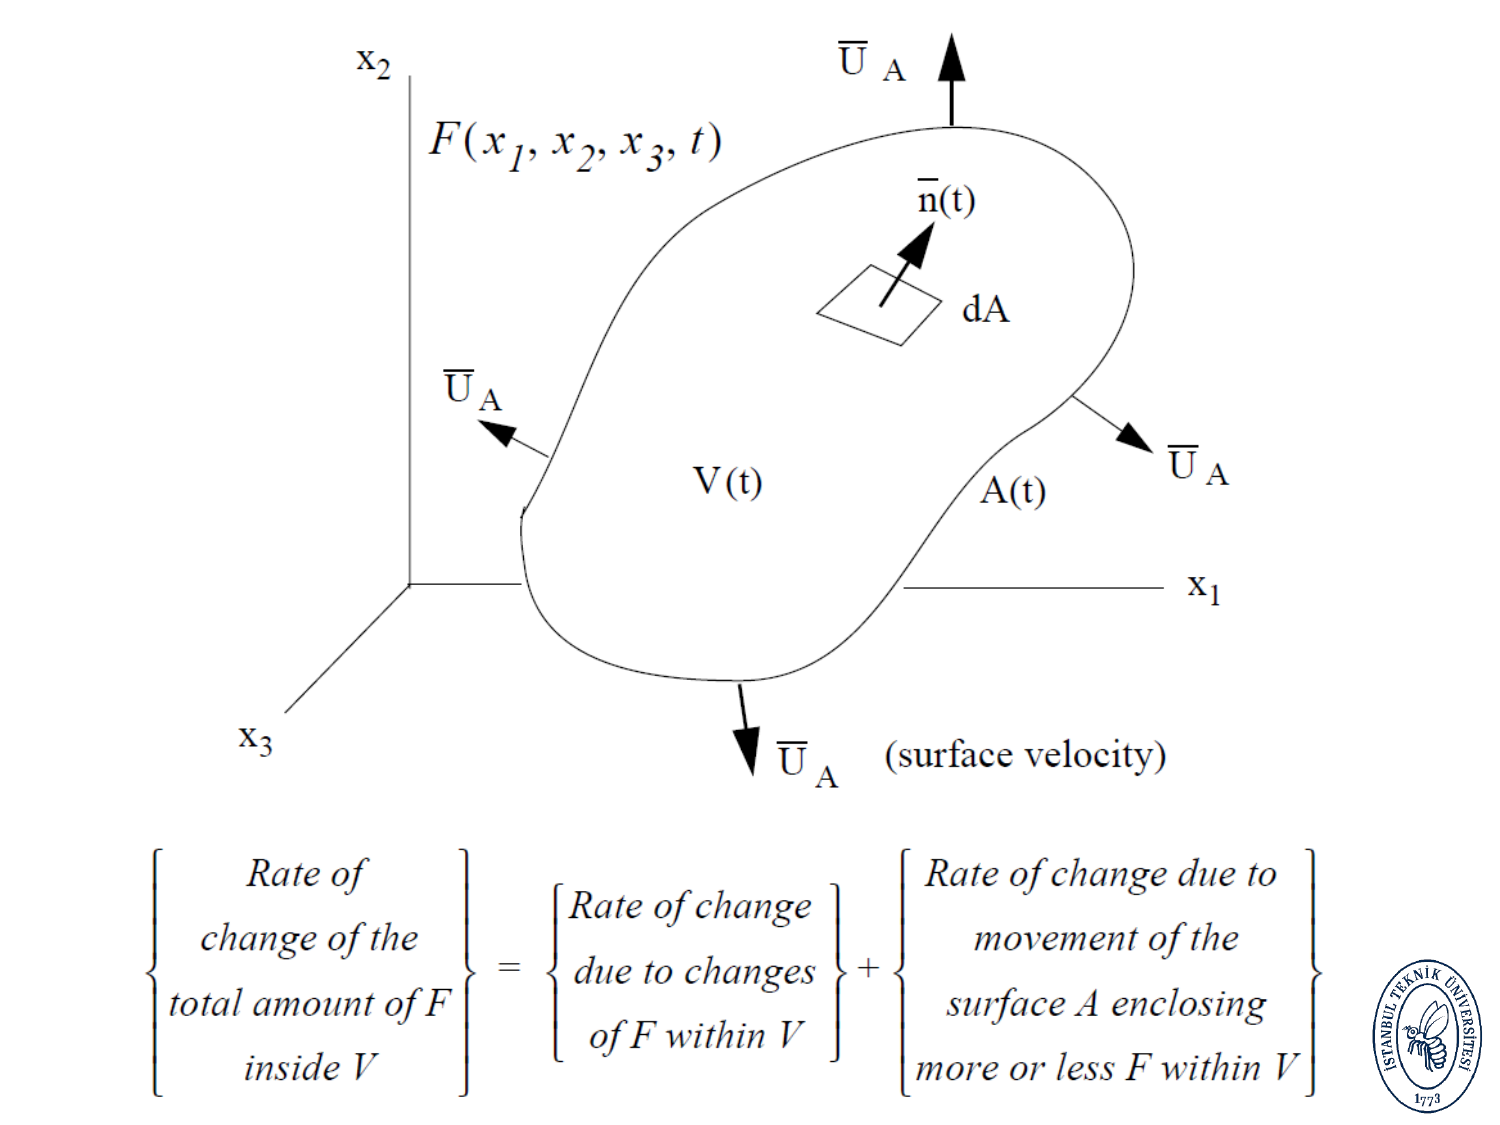
\includegraphics[width=0.78\linewidth,trim=10 30 10 50,clip]{slide15.png}
  \end{center}
  \[
    \begin{Bmatrix}
      \text{rate of change of the} \\
      \text{total amount of }F \\
      \text{inside }\Vol
    \end{Bmatrix}
    =
    \begin{Bmatrix}
      \text{rate of change} \\
      \text{due to changes} \\
      \text{of }F\text{ within }\Vol
    \end{Bmatrix}
    +
    \begin{Bmatrix}
      \text{rate of change due to} \\
      \text{movement of the surface }A \\
      \text{enclosing more or less }F
    \end{Bmatrix}
  \]
\end{frame}

% =========================================================================
% Slide 16 -- Generalised Leibnitz
% =========================================================================
\begin{frame}{Generalising the Leibnitz Theorem}
  Generalising the Leibnitz theorem we write
  \[
    \frac{\dd}{\dd t}\!\int_{\Vol(t)}\!F(\bx,t)\,\dd\Vol
      \;=\; \int_{\Vol(t)}\!\pd{F}{t}\,\dd\Vol
        \;+\; \int_{A(t)}\!F\,\bu_{A}\!\cdot\!\dd\mathbf{A}
  \]
  \begin{block}{Fixed volume\;\;($\bu_{A}=0$)}
    \[
      \frac{\dd}{\dd t}\!\int_{\Vol}\!F\,\dd\Vol
        \;=\; \int_{\Vol}\!\pd{F}{t}\,\dd\Vol
    \]
  \end{block}
  \begin{block}{Material volume\;\;($\bu_{A}=\bu$)}
    \[
      \frac{\D}{\D t}\!\int_{\Vol}\!F\,\dd\Vol
        \;=\; \int_{\Vol}\!\pd{F}{t}\,\dd\Vol
        \;+\; \int_{A}\!F\,\bu\!\cdot\!\dd\mathbf{A}
    \]
  \end{block}
\end{frame}

% =========================================================================
% Slide 17 -- Reynolds Transport Theorem
% =========================================================================
\begin{frame}{Reynolds Transport Theorem}
  Using the divergence theorem to convert the area integral into a volume
  integral:
  \[
    \boxed{\;\frac{\D}{\D t}\!\int_{\Vol}\!F(\bx,t)\,\dd\Vol
        \;=\; \int_{\Vol}\!\Bigl[\pd{F}{t} + \divg(F\bu)\Bigr]\dd\Vol\;}
  \]
  This is the \alert{Reynolds transport theorem}.
\end{frame}

% =========================================================================
% Slide 18 -- Conservation of Mass
% =========================================================================
\begin{frame}{Conservation of Mass}
  The rate of increase of mass within a fixed volume must equal the rate of
  inflow through the boundaries:
  \[
    \frac{\dd}{\dd t}\!\int_{\Vol}\!\rho\,\dd\Vol
      \;=\; -\int_{A}\!\rho\,\bu\!\cdot\!\dd\mathbf{A}
    \quad\Longrightarrow\quad
    \int_{\Vol}\!\pd{\rho}{t}\,\dd\Vol \;=\; -\int_{A}\!\rho\,\bu\!\cdot\!\dd\mathbf{A}
  \]
  Converting the area integral to a volume integral,
  \[
    \int_{\Vol}\!\Bigl[\pd{\rho}{t} + \divg(\rho\bu)\Bigr]\dd\Vol \;=\; 0
    \quad\Longrightarrow\quad
    \boxed{\;\pd{\rho}{t} + \divg(\rho\bu) \;=\; 0\;}
  \]
\end{frame}

% =========================================================================
% Slide 19 -- Species conservation (derivation)
% =========================================================================
\begin{frame}{Species Conservation}
  Following a material volume,
  \[
    \underbrace{\frac{\D}{\D t}\!\int_{\Vol}\!\rho\,Y_{m}\,\dd\Vol}_{\text{rate of change of species mass}}
      \;=\; \underbrace{\int_{A}\!\frac{\partial(\mathcal{D}\rho Y_{m})}{\partial x_{i}}\,\dd A_{i}}_{\text{diffusive mass flux into }\Vol}
        \;+\; \underbrace{\int_{\Vol}\!\dot{w}'''_{m}\,\dd\Vol}_{\text{chemical source}}
  \]
  Using the Reynolds transport theorem on the LHS,
  \[
    \frac{\D}{\D t}\!\int_{\Vol}\!\rho Y_{m}\,\dd\Vol
      \;=\; \int_{\Vol}\!\Bigl[\pd{(\rho Y_{m})}{t} + \pd{(\rho Y_{m}u_{i})}{x_{i}}\Bigr]\dd\Vol
  \]
  Converting the area integral via the divergence theorem,
  \[
    \int_{A}\!\frac{\partial(\mathcal{D}\rho Y_{m})}{\partial x_{i}}\,\dd A_{i}
      \;=\; \int_{\Vol}\!\frac{\partial}{\partial x_{i}}\!\left(\mathcal{D}\,\pd{\rho Y_{m}}{x_{i}}\right)\dd\Vol
  \]
\end{frame}

% =========================================================================
% Slide 20 -- Species final form
% =========================================================================
\begin{frame}{Species Conservation (continued)}
  Plugging in,
  \[
    \int_{\Vol}\!\Bigl[\pd{(\rho Y_{m})}{t} + \pd{(\rho Y_{m}u_{i})}{x_{i}}\Bigr]\dd\Vol
      = \int_{\Vol}\!\frac{\partial}{\partial x_{i}}\!\left(\mathcal{D}\,\pd{\rho Y_{m}}{x_{i}}\right)\dd\Vol
        + \int_{\Vol}\!\dot{w}'''_{m}\,\dd\Vol
  \]
  Rearranging and noting that the integration kernel must vanish everywhere,
  \[
    \pd{(\rho Y_{m})}{t} + \pd{}{x_{i}}\!\left(\rho Y_{m}u_{i} - \mathcal{D}\,\pd{\rho Y_{m}}{x_{i}}\right) - \dot{w}'''_{m} \;=\; 0
  \]
  yields the final form of the species conservation equation:
  \[
    \boxed{\;\pd{(\rho Y_{m})}{t} + \pd{}{x_{i}}\!\left(\rho Y_{m}u_{i} - \mathcal{D}\,\pd{\rho Y_{m}}{x_{i}}\right) \;=\; \dot{w}'''_{m}\;}
  \]
\end{frame}

% =========================================================================
% Slide 21 -- Origin of forces
% =========================================================================
\begin{frame}{Origin of Forces in a Fluid}
  \begin{block}{i. Body forces}
    Forces that arise from \emph{action at a distance}. They result from the
    medium being placed in a force field (gravitational, magnetic,
    electrostatic, electromagnetic\,\dots). Distributed throughout the mass of
    the fluid and proportional to mass.
    \medskip
    Conservative body forces can be expressed as the gradient of a potential:
    \[
      \bg \;=\; -\nabla\Pi, \qquad \Pi = g z
    \]
  \end{block}
  \begin{block}{ii. Surface forces}
    Exerted on an area element through direct contact, proportional to its
    extent and expressed per unit area. They resolve into normal and
    tangential components:
    \[
      \tau_{n} \;=\; \frac{\dd F_{n}}{\dd A}, \qquad
      \tau_{s} \;=\; \frac{\dd F_{s}}{\dd A}.
    \]
    The state of stress at a point is specified by a stress tensor with $9$
    components.
  \end{block}
\end{frame}

% =========================================================================
% Slide 22 -- Line forces
% =========================================================================
\begin{frame}{Line (Surface-Tension) Forces}
  \begin{block}{iii. Line forces}
    Surface tension forces are called \emph{line forces} because they act
    along a line and have a magnitude proportional to the extent of the line.
    They appear at the interface between a liquid and a gas, or at the
    interface between two immiscible fluids.

    \medskip
    Surface-tension forces do not appear directly in the equations of motion;
    they enter only through the boundary conditions.
  \end{block}
\end{frame}

% =========================================================================
% Slide 23 -- Stress at a point (image)
% =========================================================================
\begin{frame}{Stress at a Point}
  \begin{center}
    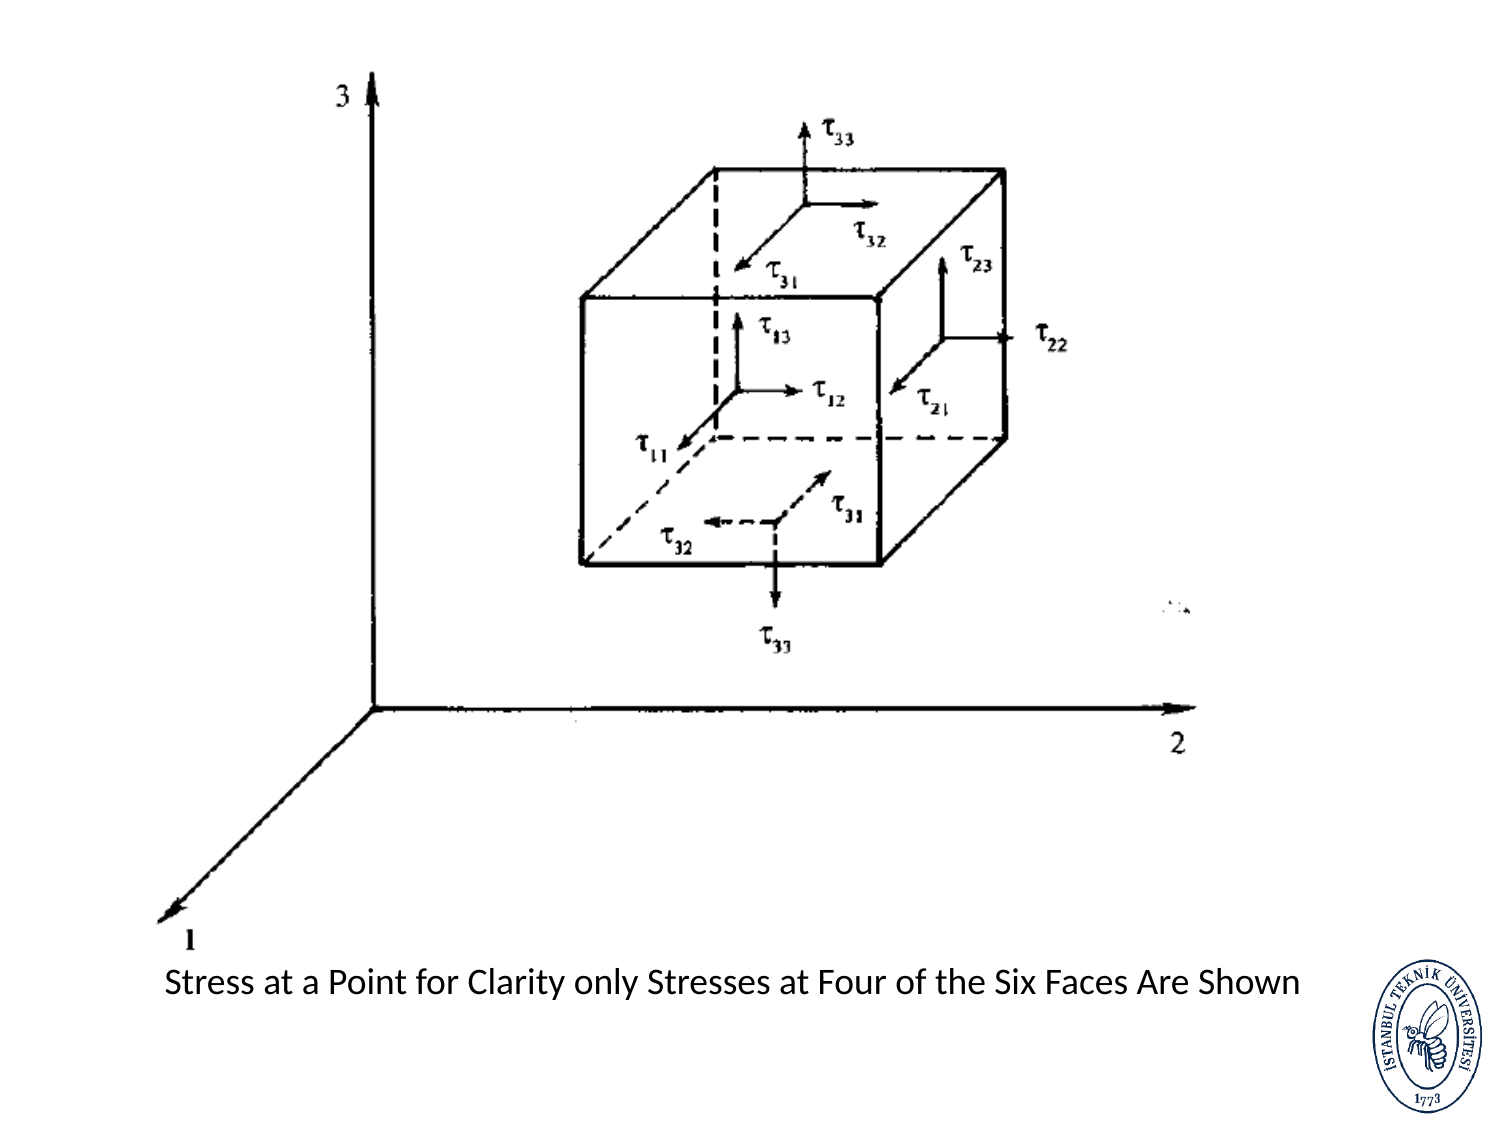
\includegraphics[width=0.6\linewidth,trim=10 40 10 60,clip]{slide23.png}
  \end{center}
  \begin{center}\footnotesize
    For clarity, only stresses at four of the six faces are shown.
  \end{center}
\end{frame}

% =========================================================================
% Slide 24 -- Symmetry of stress tensor
% =========================================================================
\begin{frame}{Proof that the Stress Tensor is Symmetric}
  Consider the torque on an element about a centroidal axis parallel to
  $x_{3}$. This torque is generated only by shear stresses in the
  $x_{1}x_{2}$ plane:
  \begin{align*}
    T &= \Bigl[\tau_{12} + \tfrac{1}{2}\,\pd{\tau_{12}}{x_{1}}\dd x_{1}\Bigr]\dd x_{2}\,\dd x_{3}\,\frac{\dd x_{1}}{2}
       + \Bigl[\tau_{12} - \tfrac{1}{2}\,\pd{\tau_{12}}{x_{1}}\dd x_{1}\Bigr]\dd x_{2}\,\dd x_{3}\,\frac{\dd x_{1}}{2} \\
      &\;-\; \Bigl[\tau_{21} + \tfrac{1}{2}\,\pd{\tau_{21}}{x_{2}}\dd x_{2}\Bigr]\dd x_{1}\,\dd x_{3}\,\frac{\dd x_{2}}{2}
            - \Bigl[\tau_{21} - \tfrac{1}{2}\,\pd{\tau_{21}}{x_{2}}\dd x_{2}\Bigr]\dd x_{1}\,\dd x_{3}\,\frac{\dd x_{2}}{2}
  \end{align*}
\end{frame}

% =========================================================================
% Slide 25 -- After cancellation
% =========================================================================
\begin{frame}{Symmetry of the Stress Tensor (continued)}
  After cancellation,
  \[
    T \;=\; (\tau_{12} - \tau_{21})\,\dd x_{1}\,\dd x_{2}\,\dd x_{3}.
  \]
  Rotational equilibrium requires $T = I\dot\omega_{3}$ with the moment of
  inertia
  \[
    I \;=\; \dd x_{1}\,\dd x_{2}\,\dd x_{3}\,\frac{\rho}{12}\bigl(\dd x_{1}^{2}+\dd x_{2}^{2}\bigr).
  \]
  Therefore
  \[
    (\tau_{12}-\tau_{21})\,\dd x_{1}\dd x_{2}\dd x_{3}
      \;=\; \frac{\rho}{12}\bigl(\dd x_{1}^{2}+\dd x_{2}^{2}\bigr)\,\dd x_{1}\dd x_{2}\dd x_{3}\,\dot\omega_{3}.
  \]
  This can be satisfied only if $\tau_{12}=\tau_{21}$. In general,
  \[
    \boxed{\;\tau_{ij} \;=\; \tau_{ji}\;}
  \]
\end{frame}


% =========================================================================
% Slide 26 -- Stress notation diagram
% =========================================================================
\begin{frame}{Stress Components on a Fluid Element}
  \begin{center}
    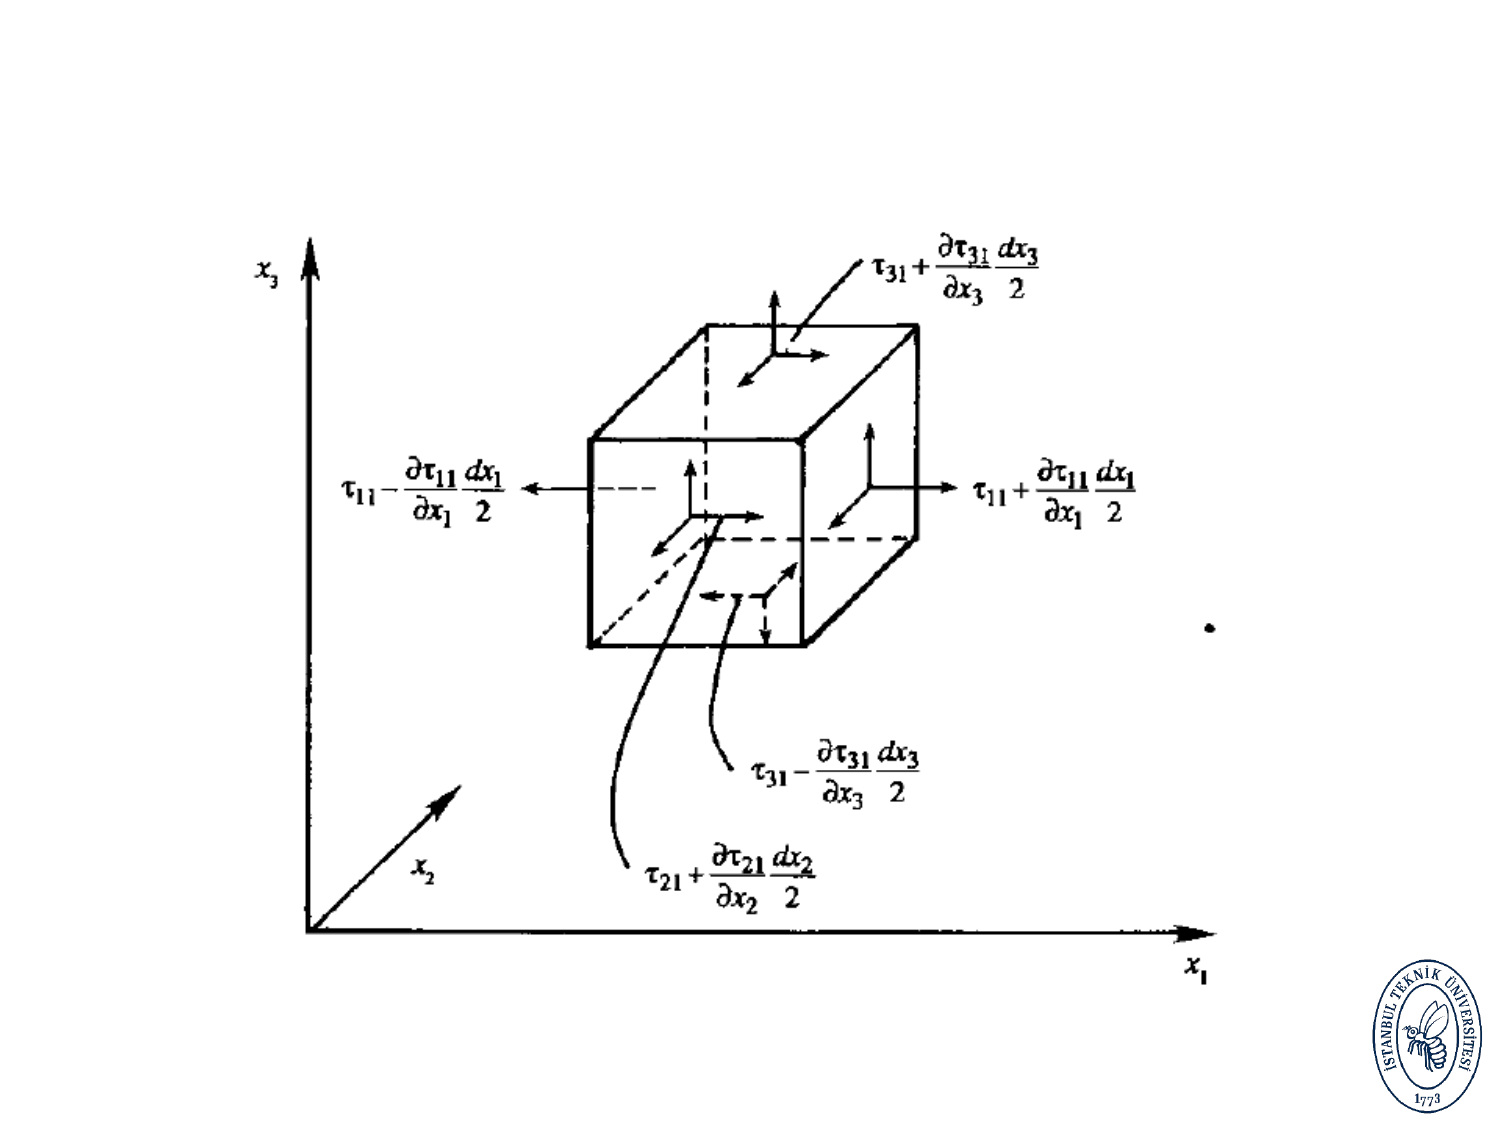
\includegraphics[width=0.7\linewidth,trim=10 40 10 60,clip]{slide26.png}
  \end{center}
\end{frame}

% =========================================================================
% Slide 27 -- Momentum integral approach -> Cauchy
% =========================================================================
\begin{frame}{Derivation of the Momentum Equation (Integral Approach)}
  In this case one does not need to consider internal stresses within the
  fluid. We simply write Newton's law for a material volume:
  \[
    \text{rate of change of momentum}
      = \text{sum of body forces} + \text{sum of surface forces}
  \]
  \[
    \frac{\D}{\D t}\!\int_{\Vol}\!\rho\,u_{i}\,\dd\Vol
      \;=\; \int_{\Vol}\!\rho g_{i}\,\dd\Vol \;+\; \int_{A}\!\tau_{ij}\,\dd A_{j}
  \]
  Converting the surface integral into a volume integral and noting that
  the integrand must vanish everywhere,
  \[
    \int_{\Vol}\!\Bigl[\rho\,\frac{\D u_{i}}{\D t} - \rho g_{i} - \pd{\tau_{ij}}{x_{j}}\Bigr]\dd\Vol \;=\; 0
  \]
  \[
    \boxed{\;\rho\,\frac{\D u_{i}}{\D t} \;=\; \rho g_{i} + \pd{\tau_{ij}}{x_{j}}\;}
    \quad\text{(\alert{Cauchy equation})}
  \]
\end{frame}

% =========================================================================
% Slide 28 -- Constitutive eq for Newtonian fluid (intro, static)
% =========================================================================
\begin{frame}{Constitutive Equation for a Newtonian Fluid}
  The relation between stress and deformation is called a \alert{constitutive
  equation}.

  \medskip
  In a fluid at rest there are only normal components of stress and the
  stress tensor is isotropic. An isotropic tensor is one whose components
  do not change under rotation. The only second-order isotropic tensor is
  the Kronecker delta:
  \[
    \delta \;=\;
    \begin{bmatrix}
      1 & 0 & 0 \\
      0 & 1 & 0 \\
      0 & 0 & 1
    \end{bmatrix}.
  \]
  Therefore the stress in a static fluid must be of the form
  \[
    \tau_{ij} \;=\; -P\,\delta_{ij}.
  \]
\end{frame}

% =========================================================================
% Slide 29 -- Deviatoric stress / strain rate decomposition
% =========================================================================
\begin{frame}{Deviatoric Stress and Strain-Rate Tensor}
  A parcel of fluid in motion develops additional stresses due to viscosity.
  Split the stress into two parts:
  \[
    \tau_{ij} \;=\; -P\,\delta_{ij} + \sigma_{ij}.
  \]
  $P$ is still the thermodynamic pressure (assuming the molecular relaxation
  time is small compared to the flow time-scale). The non-isotropic part
  $\sigma_{ij}$ is the \alert{deviatoric stress tensor}, related to velocity
  gradients. The velocity gradient tensor decomposes as
  \[
    \pd{u_{i}}{x_{j}} \;=\;
      \tfrac{1}{2}\!\Bigl(\pd{u_{i}}{x_{j}}+\pd{u_{j}}{x_{i}}\Bigr)
      + \tfrac{1}{2}\!\Bigl(\pd{u_{i}}{x_{j}}-\pd{u_{j}}{x_{i}}\Bigr).
  \]
  The anti-symmetric part is rotation without deformation and cannot
  generate stress. The stress is generated by the \alert{strain-rate tensor}
  \[
    e_{ij} \;\equiv\; \tfrac{1}{2}\!\Bigl(\pd{u_{i}}{x_{j}}+\pd{u_{j}}{x_{i}}\Bigr).
  \]
\end{frame}

% =========================================================================
% Slide 30 -- 4th order tensor relation
% =========================================================================
\begin{frame}{Linear Stress--Strain-Rate Relation}
  Assume a linear relation
  \[
    \sigma_{ij} \;=\; K_{ijmn}\,e_{mn}.
  \]
  $K_{ijmn}$ is a fourth-order tensor with $81$ components that depend on
  the local thermodynamic state. Each stress component is linearly related
  to all nine components of $e_{ij}$.

  \medskip
  An isotropic medium has no directional preference, so the stress--strain
  relationship must be independent of coordinate system rotation. Therefore
  $K_{ijmn}$ must be an \alert{isotropic tensor}.
\end{frame}

% =========================================================================
% Slide 31 -- Isotropic 4th order tensor form
% =========================================================================
\begin{frame}{Isotropic Fourth-Order Tensor}
  All isotropic tensors of even order are made up of products of the
  Kronecker delta. A fourth-order isotropic tensor has the form
  \[
    K_{ijmn} \;=\; \lambda\,\delta_{ij}\delta_{mn}
                  + \mu\,\delta_{im}\delta_{jn}
                  + \gamma\,\delta_{in}\delta_{jm}
  \]
  where $\lambda$, $\mu$, $\gamma$ depend on the local thermodynamic state.
  Symmetry of $\sigma_{ij}$ requires $\mu = \gamma$. Substituting,
  \[
    \sigma_{ij} \;=\; \bigl[\lambda\,\delta_{ij}\delta_{mn} + \mu\,(\delta_{im}\delta_{jn}+\delta_{in}\delta_{jm})\bigr]e_{mn}
  \]
  Further algebra yields
  \[
    \sigma_{ij} \;=\; 2\mu\,e_{ij} + \lambda\,e_{mm}\,\delta_{ij},
    \qquad e_{mm} \;=\; \divg\bu \quad\text{(volumetric strain rate)}.
  \]
\end{frame}

% =========================================================================
% Slide 32 -- Complete stress tensor
% =========================================================================
\begin{frame}{Complete Stress Tensor}
  The complete stress tensor becomes
  \[
    \tau_{ij} \;=\; -P\,\delta_{ij} + 2\mu\,e_{ij} + \lambda\,e_{mm}\,\delta_{ij}.
  \]
  Setting $i=j$ and summing over the repeated index,
  \[
    \tau_{ii} \;=\; -3P + (2\mu + 3\lambda)\,\divg\bu.
  \]
  Solving for pressure,
  \[
    P \;=\; -\tfrac{1}{3}\,\tau_{ii} + \!\Bigl(\tfrac{2}{3}\mu + \lambda\Bigr)\divg\bu.
  \]
  The diagonal terms of the strain-rate tensor in a flow may be unequal,
  so the stress tensor can have unequal diagonal terms because of the term
  proportional to $\mu$.
\end{frame}

% =========================================================================
% Slide 33 -- Mean pressure
% =========================================================================
\begin{frame}{Mechanical (Mean) Pressure}
  Take the average of the diagonal terms of the stress tensor and define
  the \alert{mean pressure}:
  \[
    \bar{P} \;\equiv\; -\tfrac{1}{3}\,\tau_{ii}.
  \]
  Substituting into the prior expression,
  \[
    P - \bar{P} \;=\; \!\Bigl(\tfrac{2}{3}\mu + \lambda\Bigr)\divg\bu.
  \]
  For a completely incompressible fluid one can only define a mechanical
  (mean) pressure, since there is no equation of state to determine a
  thermodynamic pressure.
\end{frame}

% =========================================================================
% Slide 34 -- Bulk viscosity
% =========================================================================
\begin{frame}{Incompressible and Compressible Forms; Bulk Viscosity}
  For incompressible fluids $e_{mm}=\divg\bu=0$, so
  \[
    \boxed{\;\tau_{ij} \;=\; -P\,\delta_{ij} + 2\mu\,e_{ij}\;}
    \quad\text{(incompressible)}.
  \]
  For a compressible fluid, the rate of expansion is related to the
  difference between the thermodynamic and mean pressures through a
  proportionality constant:
  \[
    P - \bar{P} \;=\; \kappa\,\divg\bu,
    \qquad
    \kappa \;\equiv\; \tfrac{2}{3}\mu + \lambda.
  \]
  $\kappa$ is the \alert{bulk viscosity coefficient}.
\end{frame}

% =========================================================================
% Slide 35 -- Bulk viscosity continued (table image)
% =========================================================================
\begin{frame}{Viscous Normal Force and Bulk Viscosity}
  $\kappa$ contributes only to the viscous normal force and seems to arise
  from the exchange of momentum between colliding molecules and the
  internal degrees of freedom of the molecular system.

  \begin{center}
    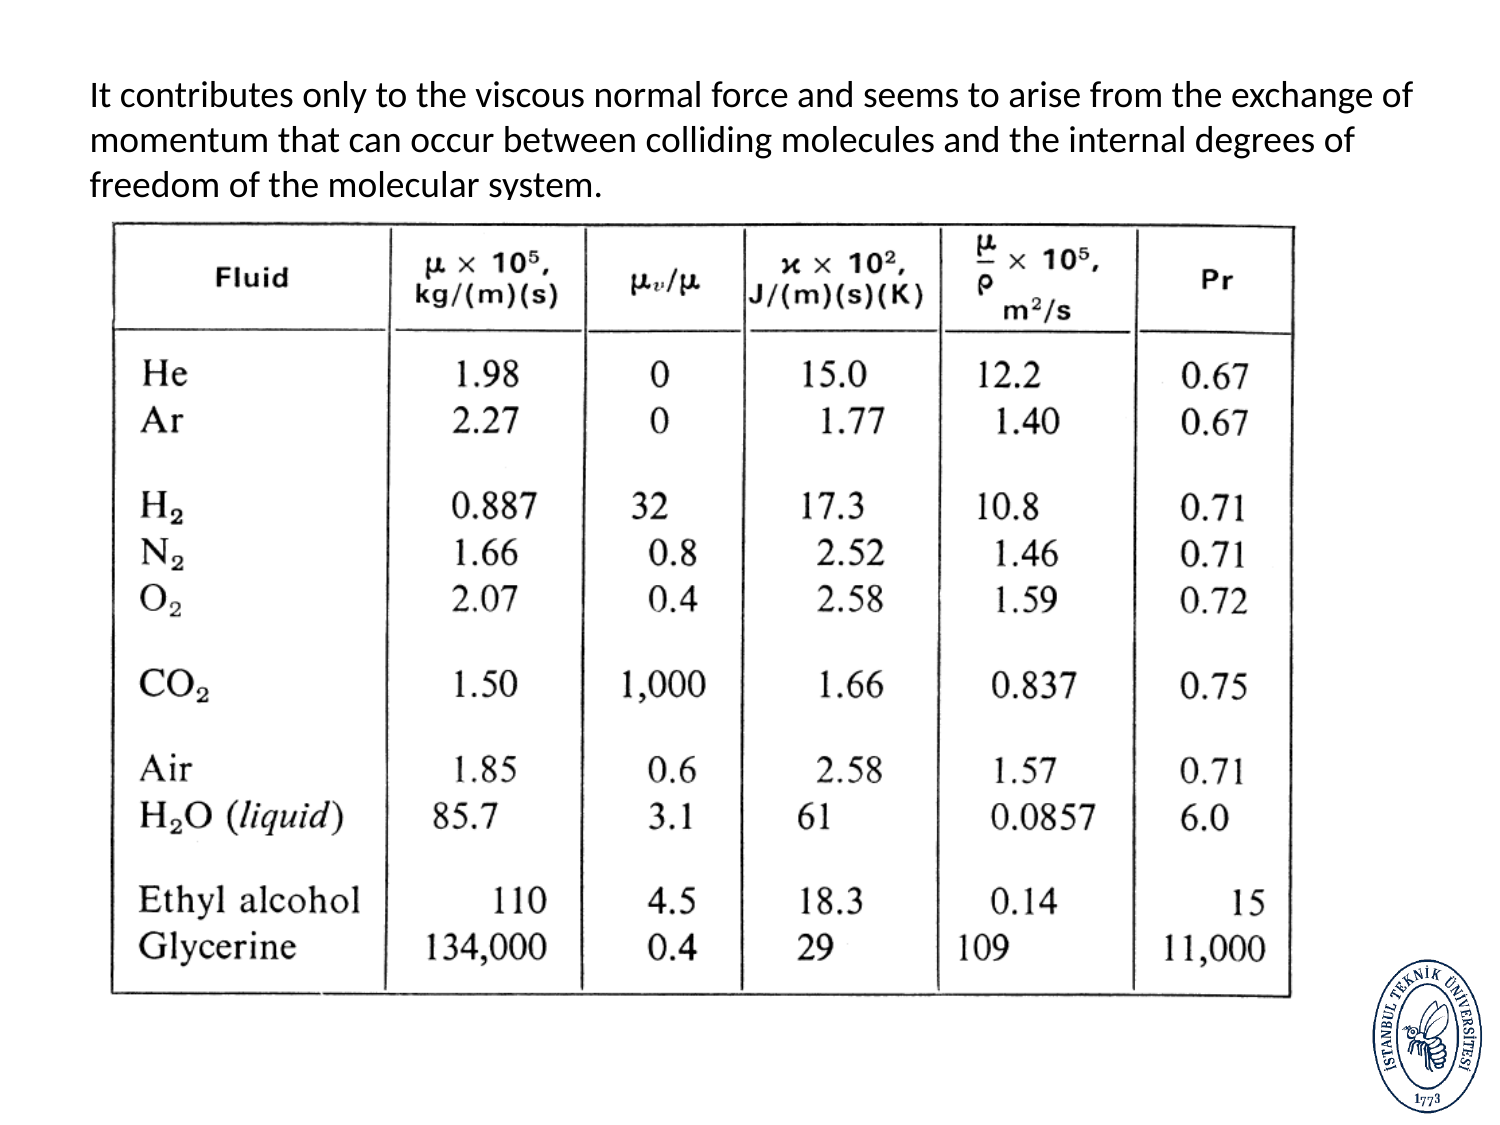
\includegraphics[width=0.65\linewidth,trim=10 40 10 40,clip]{slide35.png}
  \end{center}
\end{frame}

% =========================================================================
% Slide 36 -- Stokes hypothesis
% =========================================================================
\begin{frame}{Stokes' Hypothesis}
  In principle the bulk viscosity is a measurable quantity, yet extremely
  large values of $\D\rho/\D t$ are needed (such as within shock waves).
  Measurements are inconclusive about the nature of $\kappa$.

  \medskip
  A common assumption known as \alert{Stokes' hypothesis} is to take
  \[
    \lambda + \tfrac{2}{3}\mu \;=\; 0.
  \]
  While strictly valid only for monatomic gases, it is applied very widely
  and works well because $\divg\bu$ tends to be small outside of shock
  waves and high-Mach-number flow. With this assumption,
  \[
    \boxed{\;\tau_{ij} \;=\; -\!\Bigl(P+\tfrac{2}{3}\mu\,\divg\bu\Bigr)\delta_{ij}
                  + 2\mu\,e_{ij}\;}
    \quad\text{(compressible)}.
  \]
\end{frame}

% =========================================================================
% Slide 37 -- Newtonian fluid -- summary
% =========================================================================
\begin{frame}{Newtonian Fluid}
  The linear relation between the stress and strain-rate tensors is
  consistent with Newton's definition of viscosity in a simple parallel flow:
  \[
    \tau \;=\; \mu\,\bigl(\dd u/\dd y\bigr).
  \]
  A fluid obeying such a linear relationship is a \alert{Newtonian fluid}
  and $\mu$ depends only on the local thermodynamic state. The non-diagonal
  terms relate shear stress to strain rate. The diagonal terms,
  \[
    \tau_{11} \;=\; -P + 2\mu\!\Bigl[\pd{u_{1}}{x_{1}}-\tfrac{1}{3}\,\divg\bu\Bigr],
  \]
  state that the normal viscous stress on a plane normal to $x_{1}$ is
  proportional to the difference between the extension rate along $x_{1}$
  and the average expansion rate at the point. Only extension rates
  differing from the average generate normal viscous stress.
\end{frame}

% =========================================================================
% Slide 38 -- Navier-Stokes
% =========================================================================
\begin{frame}{Navier--Stokes Equations}
  Substituting the constitutive equation into Cauchy's equation,
  \[
    \boxed{\;\rho\,\frac{\D u_{i}}{\D t}
       \;=\; -\pd{P}{x_{i}} + \rho g_{i}
             + \pd{}{x_{j}}\!\Bigl[2\mu\,e_{ij} - \tfrac{2}{3}\mu\,(\divg\bu)\,\delta_{ij}\Bigr]\;}
  \]
  where we have noted that $\bigl(\partial P/\partial x_{j}\bigr)\delta_{ij}=\partial P/\partial x_{i}$.
  This is the general form of the Navier--Stokes equation.
\end{frame}

% =========================================================================
% Slide 39 -- Special forms of NS
% =========================================================================
\begin{frame}{Special Forms of the Navier--Stokes Equation}
  If temperature differences are small, $\mu$ can be taken outside the
  derivative:
  \[
    \rho\,\frac{\D u_{i}}{\D t}
       \;=\; -\pd{P}{x_{i}} + \rho g_{i}
             + \mu\!\left[\nabla^{2} u_{i} - \tfrac{1}{3}\,\pd{}{x_{i}}(\divg\bu)\right].
  \]
  For incompressible fluids $\divg\bu=0$:
  \[
    \rho\,\frac{\D u_{i}}{\D t}
       \;=\; -\pd{P}{x_{i}} + \rho g_{i} + \mu\,\nabla^{2} u_{i}.
  \]
  If viscous effects are negligible (\alert{Euler equation}):
  \[
    \rho\,\frac{\D u_{i}}{\D t}
       \;=\; -\pd{P}{x_{i}} + \rho g_{i}.
  \]
\end{frame}

% =========================================================================
% Slide 40 -- Thermodynamic equilibrium
% =========================================================================
\begin{frame}{Thermodynamic Equilibrium}
  When a system with non-uniform properties is isolated from its
  surroundings, those properties generally change with time. Pressure
  variations cause motion until \alert{mechanical equilibrium} is reached.

  \medskip
  Temperature variations may be coupled with mechanical motion or evolve on
  a different time-scale; when all temperature changes cease the system is
  in \alert{thermal equilibrium}.

  \medskip
  Chemical reactions occur on a third time-scale set by the reactant
  nature, often much shorter than the mechanical and thermal time-scales.
  When all chemical activity ceases, \alert{chemical equilibrium} is
  reached.

  \medskip
  A system simultaneously in mechanical, thermal and chemical equilibrium
  is in \alert{thermodynamic equilibrium}.
\end{frame}

% =========================================================================
% Slide 41 -- First Law
% =========================================================================
\begin{frame}{The First Law of Thermodynamics}
  The basis of energy conservation for a fluid is the first law of
  thermodynamics. In its most elementary form, for a system,
  \[
    \dd E \;=\; \delta Q - \delta W
  \]
  with
  \begin{itemize}
    \item $E$ = total energy of the system,
    \item $Q$ = heat transferred to the system,
    \item $W$ = work done by the system on the surroundings.
  \end{itemize}
  Energy is a state variable, hence $\dd E$ is an exact differential. Heat
  added and work done depend on the process, so they are written as
  \emph{inexact} differentials $\delta Q$ and $\delta W$.
\end{frame}

% =========================================================================
% Slide 42 -- First Law for moving fluid
% =========================================================================
\begin{frame}{The First Law for a Moving Fluid}
  Assuming the flow remains close to thermodynamic equilibrium, we can
  regard it as quasi-steady (in the thermodynamic sense) and rewrite
  conservation of energy as a differential equation:
  \[
    \frac{\dd E}{\dd t} \;=\; \dot{Q} - \dot{W}
  \]
  with
  \[
    \dot{Q} \;\equiv\; \delta Q/\dd t, \qquad
    \dot{W} \;\equiv\; \delta W/\dd t.
  \]
\end{frame}

% =========================================================================
% Slide 43 -- Integral energy equation setup
% =========================================================================
\begin{frame}{Integral Form of the Energy Equation}
  Consider conservative body forces with a time-independent potential. The
  total energy per unit mass of a moving fluid element is $e+k$, where $e$
  is the internal energy and
  \[
    k \;\equiv\; \tfrac{1}{2}\,u_{i}u_{i}
            \;=\; \tfrac{1}{2}(u_{1}^{2}+u_{2}^{2}+u_{3}^{2})
  \]
  is the kinetic energy per unit mass.

  \medskip
  The stress tensor acting on the surface and the body forces both do work
  on the control volume. In addition, there may be heat flux (species
  diffusion plus conduction) through the surface into the volume.
\end{frame}

% =========================================================================
% Slide 44 -- Following a material volume
% =========================================================================
\begin{frame}{Energy Equation: Material Volume}
  Following a material volume,
  \[
    \frac{\D}{\D t}\!\int_{\Vol}\!\rho(e+k)\,\dd\Vol
      \;=\; \dot{Q} - \dot{W}.
  \]
  Using the Reynolds transport theorem on the LHS,
  \[
    \frac{\D}{\D t}\!\int_{\Vol}\!\rho(e+k)\,\dd\Vol
      \;=\; \int_{\Vol}\!\Bigl[\pd{\rho(e+k)}{t} + \divg\bigl(\rho(e+k)\bu\bigr)\Bigr]\dd\Vol.
  \]
  In index notation,
  \[
    \frac{\D}{\D t}\!\int_{\Vol}\!\rho(e+k)\,\dd\Vol
      \;=\; \int_{\Vol}\!\Bigl[\pd{\rho(e+k)}{t} + \pd{\rho(e+k)u_{j}}{x_{j}}\Bigr]\dd\Vol.
  \]
\end{frame}

% =========================================================================
% Slide 45 -- Plugging into energy eq
% =========================================================================
\begin{frame}{Energy Equation: Work by Surface Forces}
  Plugging into the energy equation,
  \[
    \int_{\Vol}\!\Bigl[\pd{\rho(e+k)}{t} + \pd{\rho(e+k)u_{i}}{x_{i}}\Bigr]\dd\Vol
      \;=\; \dot{Q} - \dot{W}.
  \]
  The rate of work done on the material volume can be expressed as
  \[
    \dot{W} \;=\; -\int_{\Vol}\!\rho g_{i}\,u_{i}\,\dd\Vol \;-\; \int_{A}\!\tau_{ij}\,u_{i}\,\dd A_{j}.
  \]
  Using the divergence theorem,
  \[
    \dot{W} \;=\; -\int_{\Vol}\!\rho g_{i}\,u_{i}\,\dd\Vol
                  \;-\; \int_{\Vol}\!\pd{(u_{i}\tau_{ij})}{x_{j}}\,\dd\Vol.
  \]
\end{frame}

% =========================================================================
% Slide 46 -- Chain rule split
% =========================================================================
\begin{frame}{Splitting the Surface Work}
  Using the chain rule on the work done by surface forces per unit time,
  \[
    \pd{(u_{i}\tau_{ij})}{x_{j}}
      \;=\; \underbrace{\tau_{ij}\,\pd{u_{i}}{x_{j}}}_{\text{deformation}}
        \;+\; \underbrace{u_{i}\,\pd{\tau_{ij}}{x_{j}}}_{\text{increase of KE}}
  \]
  The last term increases the kinetic energy of the element. The remainder
  can only deform the element and increase its internal energy.

  \medskip
  Using the symmetry of $\tau_{ij}$ and the Newtonian constitutive law,
  \[
    \tau_{ij}\,\pd{u_{i}}{x_{j}}
      \;=\; \tau_{ij}\,e_{ij}
      \;=\; \Bigl[-P\,\delta_{ij} + 2\mu\,e_{ij} - \tfrac{2}{3}\mu\,(\divg\bu)\,\delta_{ij}\Bigr]\,e_{ij}.
  \]
\end{frame}

% =========================================================================
% Slide 47 -- Viscous dissipation
% =========================================================================
\begin{frame}{Viscous Dissipation}
  Deformation work becomes
  \[
    \tau_{ij}\,e_{ij} \;=\; -P\,(\divg\bu) + 2\mu\,e_{ij}\,e_{ij} - \tfrac{2}{3}\mu\,(\divg\bu)^{2}
  \]
  where we have used $e_{mm}=\divg\bu$. Denoting the viscous term by $\phi$,
  \[
    \phi \;\equiv\; 2\mu\,e_{ij}\,e_{ij} - \tfrac{2}{3}\mu\,(\divg\bu)^{2}
        \;=\; 2\mu\,\Bigl[e_{ij}-\tfrac{1}{3}\,(\divg\bu)\,\delta_{ij}\Bigr]\,e_{ij}.
  \]
  $\phi$ is the rate of \alert{viscous dissipation} of kinetic energy per
  unit volume. It is proportional to the square of the velocity gradients
  and is more pronounced in regions of high shear (e.g.\ a hot lubricant in
  a bearing, or burning of a spacecraft surface upon atmospheric reentry):
  \[
    \tau_{ij}\,e_{ij} \;=\; -P\,(\divg\bu) + \phi.
  \]
\end{frame}

% =========================================================================
% Slide 48 -- Collecting terms
% =========================================================================
\begin{frame}{Collecting Terms}
  Further arranging,
  \[
    \int_{\Vol}\!\Bigl[\pd{\rho(e+k)}{t} + \pd{\rho(e+k)u_{i}}{x_{i}}
      - \rho g_{i}u_{i} - u_{i}\,\pd{\tau_{ij}}{x_{j}}
      + P\,\pd{u_{j}}{x_{j}} - \phi\Bigr]\dd\Vol \;=\; \dot{Q}.
  \]
  Collecting some terms,
  \[
    \int_{\Vol}\!\Bigl[\pd{\rho(e+k+P/\rho)}{t} + \pd{\rho(e+k+P/\rho)u_{i}}{x_{i}}
       - \rho g_{i}u_{i} - u_{i}\,\pd{\tau_{ij}}{x_{j}} - \phi\Bigr]\dd\Vol \;=\; \dot{Q}.
  \]
\end{frame}

% =========================================================================
% Slide 49 -- Enthalpy and total enthalpy
% =========================================================================
\begin{frame}{Enthalpy and Total Enthalpy}
  Invoking the definition of enthalpy $h \equiv e + P/\rho$,
  \[
    \int_{\Vol}\!\Bigl[\pd{\rho(h+k)}{t} + \pd{\rho(h+k)u_{i}}{x_{i}}
       - \rho g_{i}u_{i} - u_{i}\,\pd{\tau_{ij}}{x_{j}} - \phi\Bigr]\dd\Vol \;=\; \dot{Q}.
  \]
  Using the total enthalpy $H \equiv h + k$,
  \[
    \int_{\Vol}\!\Bigl[\pd{\rho H}{t} + \pd{\rho H u_{i}}{x_{i}}
       - \pd{P}{t} - \rho g_{i}u_{i} - u_{i}\,\pd{\tau_{ij}}{x_{j}} - \phi\Bigr]\dd\Vol \;=\; \dot{Q}.
  \]
\end{frame}

% =========================================================================
% Slide 50 -- Heat addition term
% =========================================================================
\begin{frame}{Rate of Heat Added to the Material Volume}
  The rate of heat added to the material volume is
  \[
    \dot{Q} \;=\; \int_{A}\! q_{i}\,\dd A_{i}, \qquad
    q_{i} \;=\; -k\,\pd{T}{x_{i}} - \sum_{m}\!\Bigl(\rho\mathcal{D}\,\pd{Y_{m}}{x_{i}}\,h_{m}\Bigr)
  \]
  where $q_{i}$ is the heat-flux vector (conduction + species diffusion).
  Using the divergence theorem,
  \[
    \dot{Q} \;=\; \int_{\Vol}\!\Bigl[\pd{}{x_{i}}\!\Bigl(k\,\pd{T}{x_{i}}\Bigr)
                + \pd{}{x_{i}}\!\Bigl(\sum_{m}\rho\mathcal{D}\,\pd{Y_{m}}{x_{i}}\,h_{m}\Bigr)\Bigr]\dd\Vol.
  \]
\end{frame}

% =========================================================================
% Slide 51 -- Final energy equation
% =========================================================================
\begin{frame}{Conservation of Energy: Final Form}
  Arranging and noting that the integration kernel must vanish everywhere,
  \[
    \scriptsize
    \boxed{\;
      \pd{\rho H}{t} + \pd{\rho H u_{j}}{x_{j}}
        \;=\; \pd{P}{t} + \rho g_{i}u_{i} + u_{i}\,\pd{\tau_{ij}}{x_{j}} + \phi
              + \pd{}{x_{i}}\!\Bigl(k\,\pd{T}{x_{i}}\Bigr)
              + \pd{}{x_{i}}\!\Bigl(\sum_{m}\rho\mathcal{D}\,\pd{Y_{m}}{x_{i}}\,h_{m}\Bigr)
    \;}
  \]
\end{frame}

% =========================================================================
% Slide 52 -- Summary of equations
% =========================================================================
\begin{frame}{Summary of Equations}
  \footnotesize
  \[
    \pd{\rho}{t} + \pd{\rho u_{i}}{x_{i}} \;=\; 0
  \]
  \[
    \pd{(\rho Y_{m})}{t} + \pd{}{x_{i}}\!\Bigl(\rho Y_{m}u_{i} - \mathcal{D}\,\pd{\rho Y_{m}}{x_{i}}\Bigr)
      \;=\; \dot{w}'''_{m}
  \]
  \[
    \rho\,\frac{\D u_{i}}{\D t}
      \;=\; -\pd{P}{x_{i}} + \rho g_{i}
            + \pd{}{x_{j}}\!\Bigl[2\mu\,e_{ij} - \tfrac{2}{3}\mu\,(\divg\bu)\,\delta_{ij}\Bigr]
  \]
  \[
    \pd{\rho H}{t} + \pd{\rho H u_{j}}{x_{j}}
      \;=\; \pd{P}{t} + \rho g_{i}u_{i} + u_{i}\,\pd{\tau_{ij}}{x_{j}} + \phi
            + \pd{}{x_{i}}\!\Bigl(k\,\pd{T}{x_{i}}\Bigr)
            + \pd{}{x_{i}}\!\Bigl(\sum_{m}\rho\mathcal{D}\,\pd{Y_{m}}{x_{i}}\,h_{m}\Bigr)
  \]
\end{frame}

% =========================================================================
% Slide 53 -- Elementary reactions
% =========================================================================
\begin{frame}{Elementary Reactions and Reaction Rates}
  An arbitrary bimolecular reaction is expressed as
  \[
    A + B \;\longrightarrow\; C + D,
    \qquad
    \frac{\dd[A]}{\dd t} \;=\; -k_{\text{bimolec}}(T)\,[A][B].
  \]
  $k_{\text{bimolec}}$ is the rate coefficient (function of temperature),
  with units $\text{m}^{3}/(\text{kmol}\!\cdot\!\text{s})$. We skip the
  theoretical basis for $k$.

  \medskip
  If the temperature range is not too large, the bimolecular rate
  coefficient is given by the empirical \alert{Arrhenius form}
  \[
    k(T) \;=\; A\,\exp(-E_{A}/R_{u}T).
  \]
  $A$ is the pre-exponential (frequency) factor. Current practice commonly
  uses the three-parameter form
  \[
    k(T) \;=\; A\,T^{b}\,\exp(-E_{A}/R_{u}T)
  \]
  where $A$, $b$ and $E_{A}$ are empirical parameters.
\end{frame}

% =========================================================================
% Slide 54 -- H2-O2 rate table (image)
% =========================================================================
\begin{frame}{Recommended H$_{2}$--O$_{2}$ Reaction Rate Coefficients}
  \begin{center}
    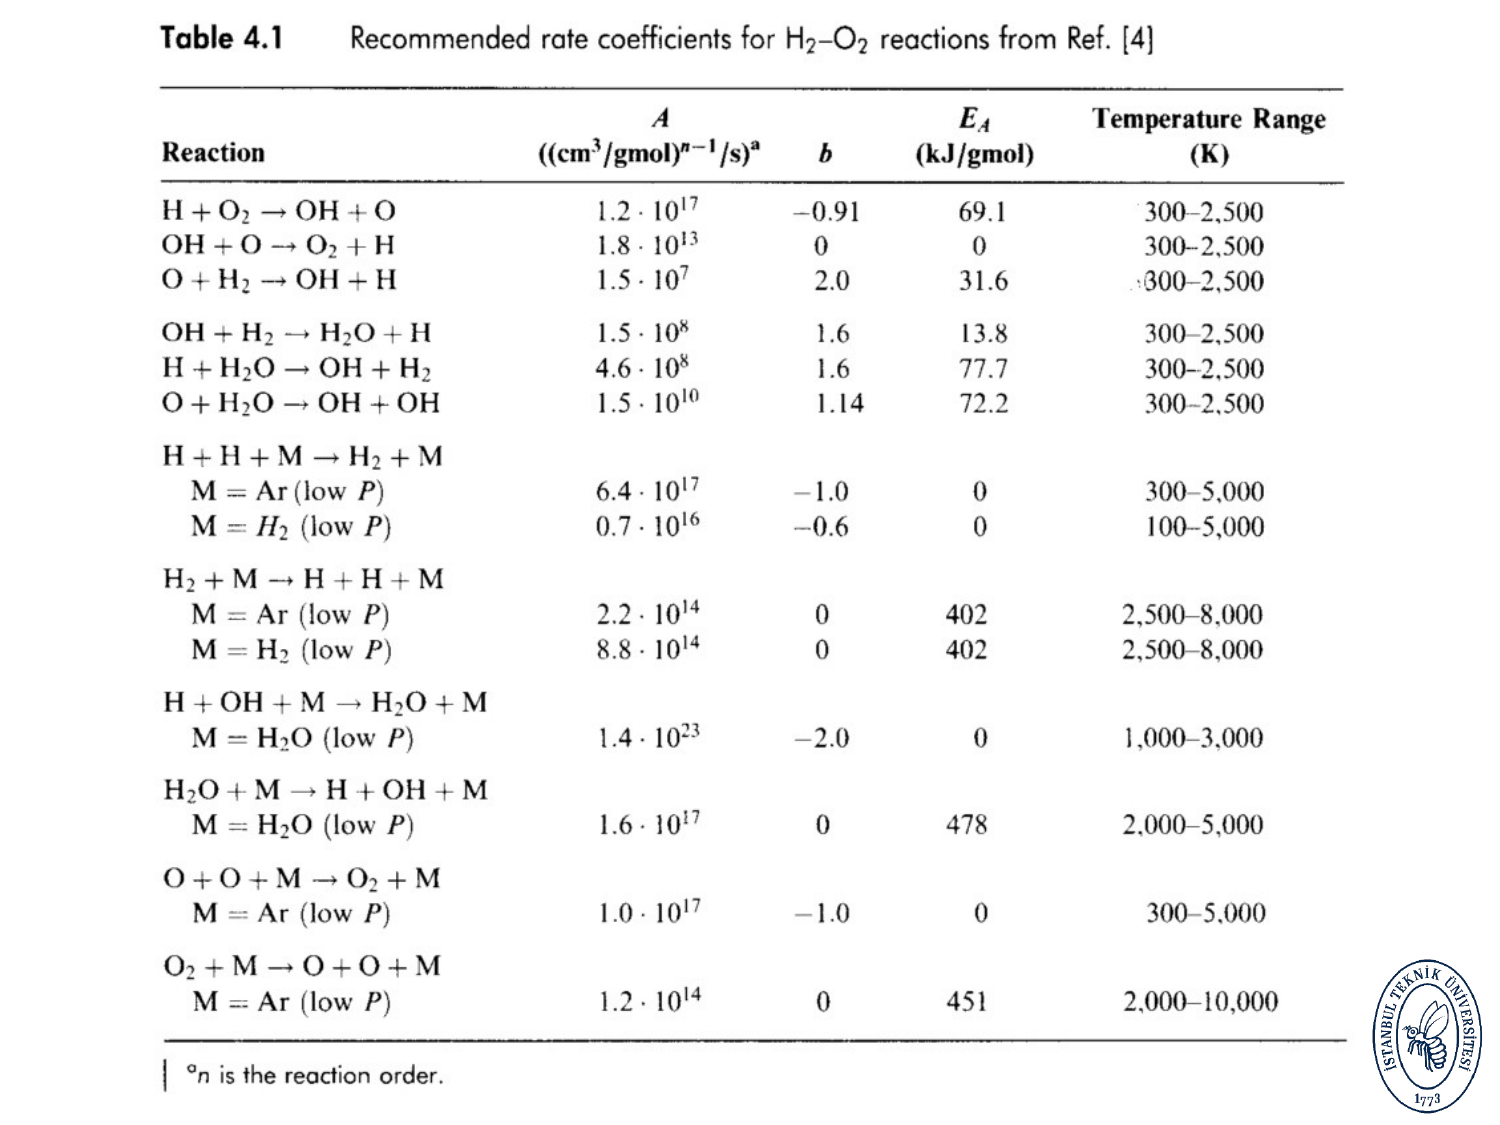
\includegraphics[width=0.95\linewidth,trim=10 40 10 40,clip]{slide54.png}
  \end{center}
\end{frame}

% =========================================================================
% Slide 55 -- Other elementary reactions
% =========================================================================
\begin{frame}{Other Elementary Reactions}
  \begin{block}{Unimolecular reactions (isomerisation or decomposition)}
    \[
      A \;\longrightarrow\; B, \qquad A \;\longrightarrow\; B + C.
    \]
  \end{block}
  \begin{block}{Termolecular reactions}
    Three reactant species; the reverse of unimolecular reactions at low
    pressures:
    \[
      A + B + M \;\longrightarrow\; C + M.
    \]
    They are third-order, with rate
    \[
      \frac{\dd[A]}{\dd t} \;=\; -k_{\text{ter}}\,[A][B][M].
    \]
    $M$ may be any molecule and is often referred to as a \emph{third body}.
    In radical--radical reactions, the third body is required to carry away
    the energy liberated in forming the stable species.
  \end{block}
\end{frame}

% =========================================================================
% Slide 56 -- Multistep mechanism
% =========================================================================
\begin{frame}{A Simple Multistep Mechanism}
  The collection of elementary reactions necessary to describe an overall
  reaction is called a \alert{reaction mechanism}.
  \begin{align*}
    H_{2} + O_{2} &\;\longleftrightarrow\; HO_{2} + H && (\text{R.1}) \\
    H + O_{2} &\;\longleftrightarrow\; OH + O && (\text{R.2}) \\
    OH + H_{2} &\;\longleftrightarrow\; H_{2}O + H && (\text{R.3}) \\
    H + O_{2} + M &\;\longleftrightarrow\; HO_{2} + M && (\text{R.4})
  \end{align*}
\end{frame}

% =========================================================================
% Slide 57 -- Net production rates
% =========================================================================
\begin{frame}{Net Production Rates}
  \[
    \pd{(\rho Y_{m})}{t} + \pd{}{x_{i}}\!\Bigl(\rho Y_{m}u_{i} - \mathcal{D}\,\pd{\rho Y_{m}}{x_{i}}\Bigr) = \dot{w}'''_{m}
  \]
  \footnotesize
  \begin{align*}
    \frac{\dd[O_{2}]}{\dd t} &= k_{r1}[HO_{2}][H] + k_{r2}[OH][O] + k_{r4}[HO_{2}][M] \\
                              &\quad - k_{f1}[H_{2}][O_{2}] - k_{f2}[H][O_{2}] - k_{f4}[H][O_{2}][M] - \cdots \\[4pt]
    \frac{\dd[H]}{\dd t}     &= k_{f1}[H_{2}][O_{2}] + k_{f2}[O_{2}][H] \\
                              &\quad + k_{f3}[OH][H_{2}] + k_{r4}[HO_{2}][M] \\
                              &\quad - k_{r1}[HO_{2}][H] - k_{r3}[H_{2}O][H] \\
                              &\quad - k_{r2}[O][H_{2}] - k_{f4}[H][O_{2}][M] - \cdots
  \end{align*}
\end{frame}

% =========================================================================
% Slide 58 -- Compact notation
% =========================================================================
\begin{frame}{Compact Notation}
  Since mechanisms may involve many elementary steps and many species, a
  compact notation is used:
  \[
    \sum_{j=1}^{N}\!\nu'_{ji}X_{j} \;\longleftrightarrow\; \sum_{j=1}^{N}\!\nu''_{ji}X_{j}, \quad i=1,2,\dots,L
  \]
  with $\nu'_{ji}$ the stoichiometric coefficients on the reactants side
  and $\nu''_{ji}$ those on the products side.

  \begin{center}\footnotesize
  \begin{tabular}{cl@{\hskip 24pt}cl}
    \toprule
    $j$ & Species & $i$ & Reaction \\ \midrule
    1 & $O_{2}$  & 1 & R.1 \\
    2 & $H_{2}$  & 2 & R.2 \\
    3 & $H_{2}O$ & 3 & R.3 \\
    4 & $HO_{2}$ & 4 & R.4 \\
    5 & $O$      &   &     \\
    6 & $H$      &   &     \\
    7 & $OH$     &   &     \\
    8 & $M$      &   &     \\
    \bottomrule
  \end{tabular}
  \end{center}
\end{frame}

% =========================================================================
% Slide 59 -- Stoich matrices
% =========================================================================
\begin{frame}{Stoichiometric Matrices}
  \[
    \nu'_{ji} \;=\;
    \begin{bmatrix}
      1 & 1 & 0 & 1 \\
      1 & 0 & 1 & 0 \\
      0 & 0 & 0 & 0 \\
      0 & 0 & 0 & 0 \\
      0 & 0 & 0 & 0 \\
      0 & 1 & 0 & 1 \\
      0 & 0 & 1 & 0 \\
      0 & 0 & 0 & 1
    \end{bmatrix},
    \qquad
    \nu''_{ji} \;=\;
    \begin{bmatrix}
      0 & 0 & 0 & 0 \\
      0 & 0 & 0 & 0 \\
      0 & 0 & 1 & 0 \\
      1 & 0 & 0 & 1 \\
      0 & 1 & 0 & 0 \\
      1 & 0 & 1 & 0 \\
      0 & 1 & 0 & 0 \\
      0 & 0 & 0 & 1
    \end{bmatrix}
  \]
  \[
    \dot{\omega}_{j} \;=\; \sum_{i=1}^{L}\!\nu_{ji}\,q_{i} \quad\text{for } j=1,2,\dots,N
  \]
  where
  \[
    \nu_{ji} \;\equiv\; \nu''_{ji} - \nu'_{ji}, \qquad
    q_{i} \;=\; k_{f i}\!\prod_{j=1}^{N}\![X_{j}]^{\nu'_{ji}} - k_{r i}\!\prod_{j=1}^{N}\![X_{j}]^{\nu''_{ji}}
  \]
  and $\dot{\omega}_{j} \equiv \dd[X_{j}]/\dd t$.
\end{frame}

% =========================================================================
% Slide 60 -- GRI Mech 3.0 table 1 (image)
% =========================================================================
\begin{frame}{GRI--Mech 3.0 for Methane Combustion (1/4)}
  \begin{center}
    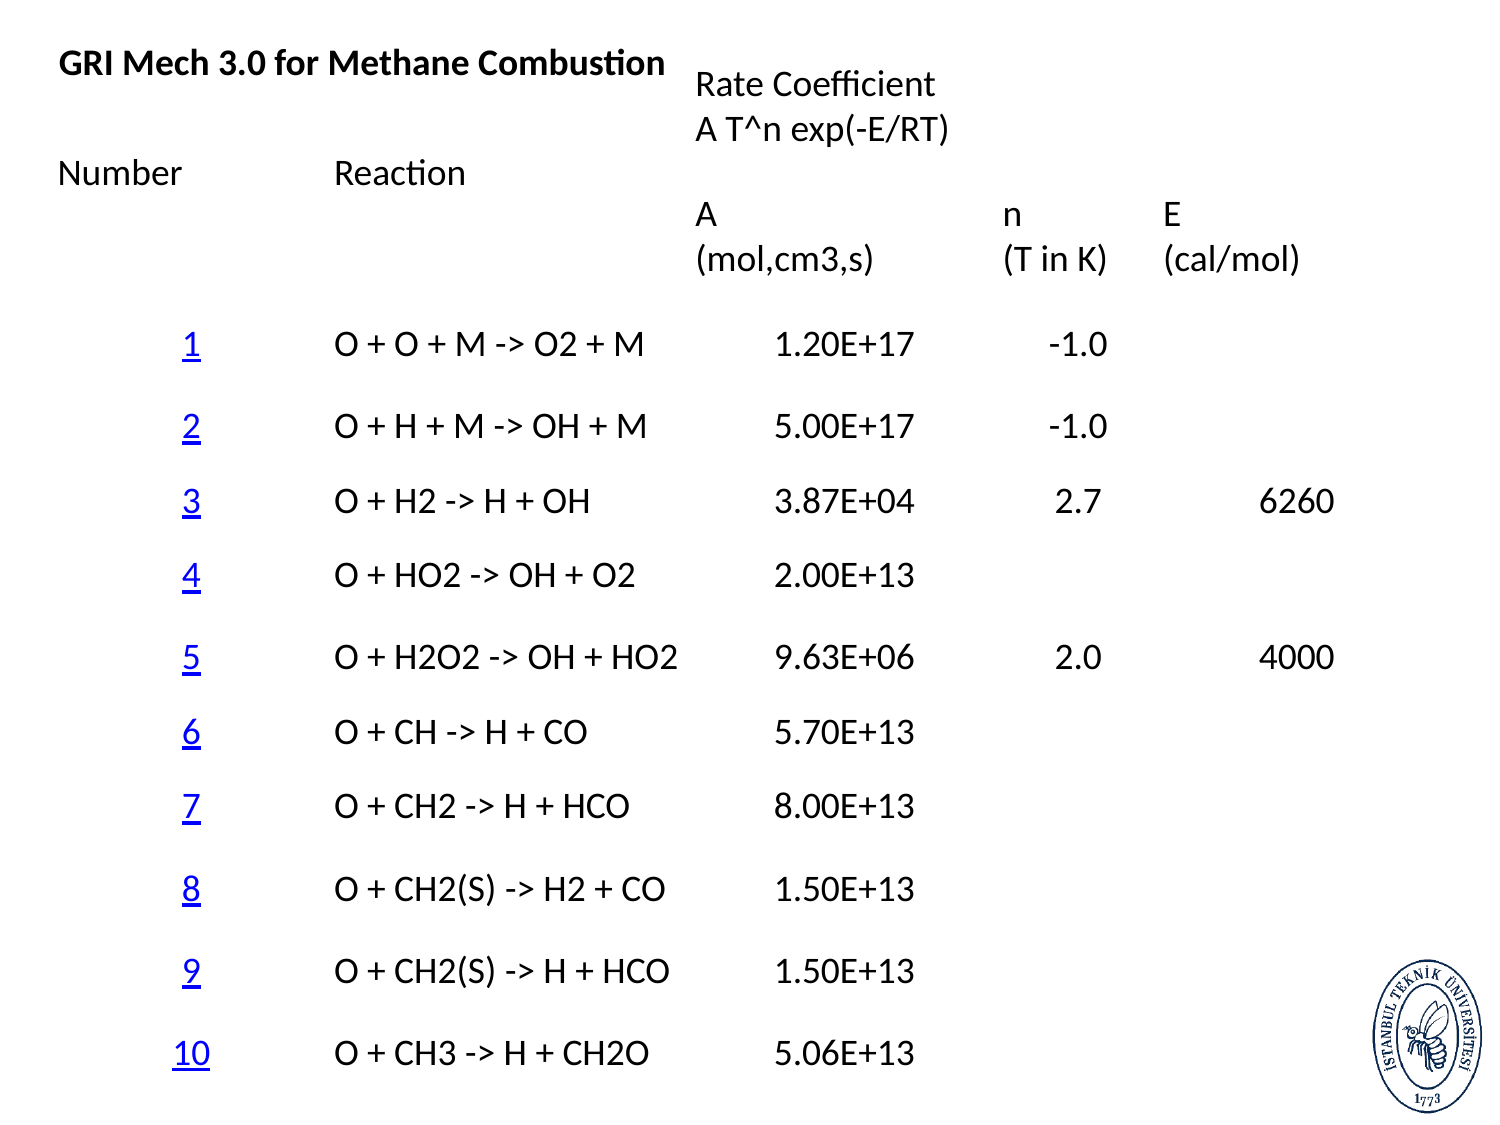
\includegraphics[width=0.95\linewidth,trim=10 40 10 40,clip]{slide60.png}
  \end{center}
\end{frame}

% =========================================================================
% Slide 61 -- GRI Mech 3.0 table 2
% =========================================================================
\begin{frame}{GRI--Mech 3.0 for Methane Combustion (2/4)}
  \begin{center}
    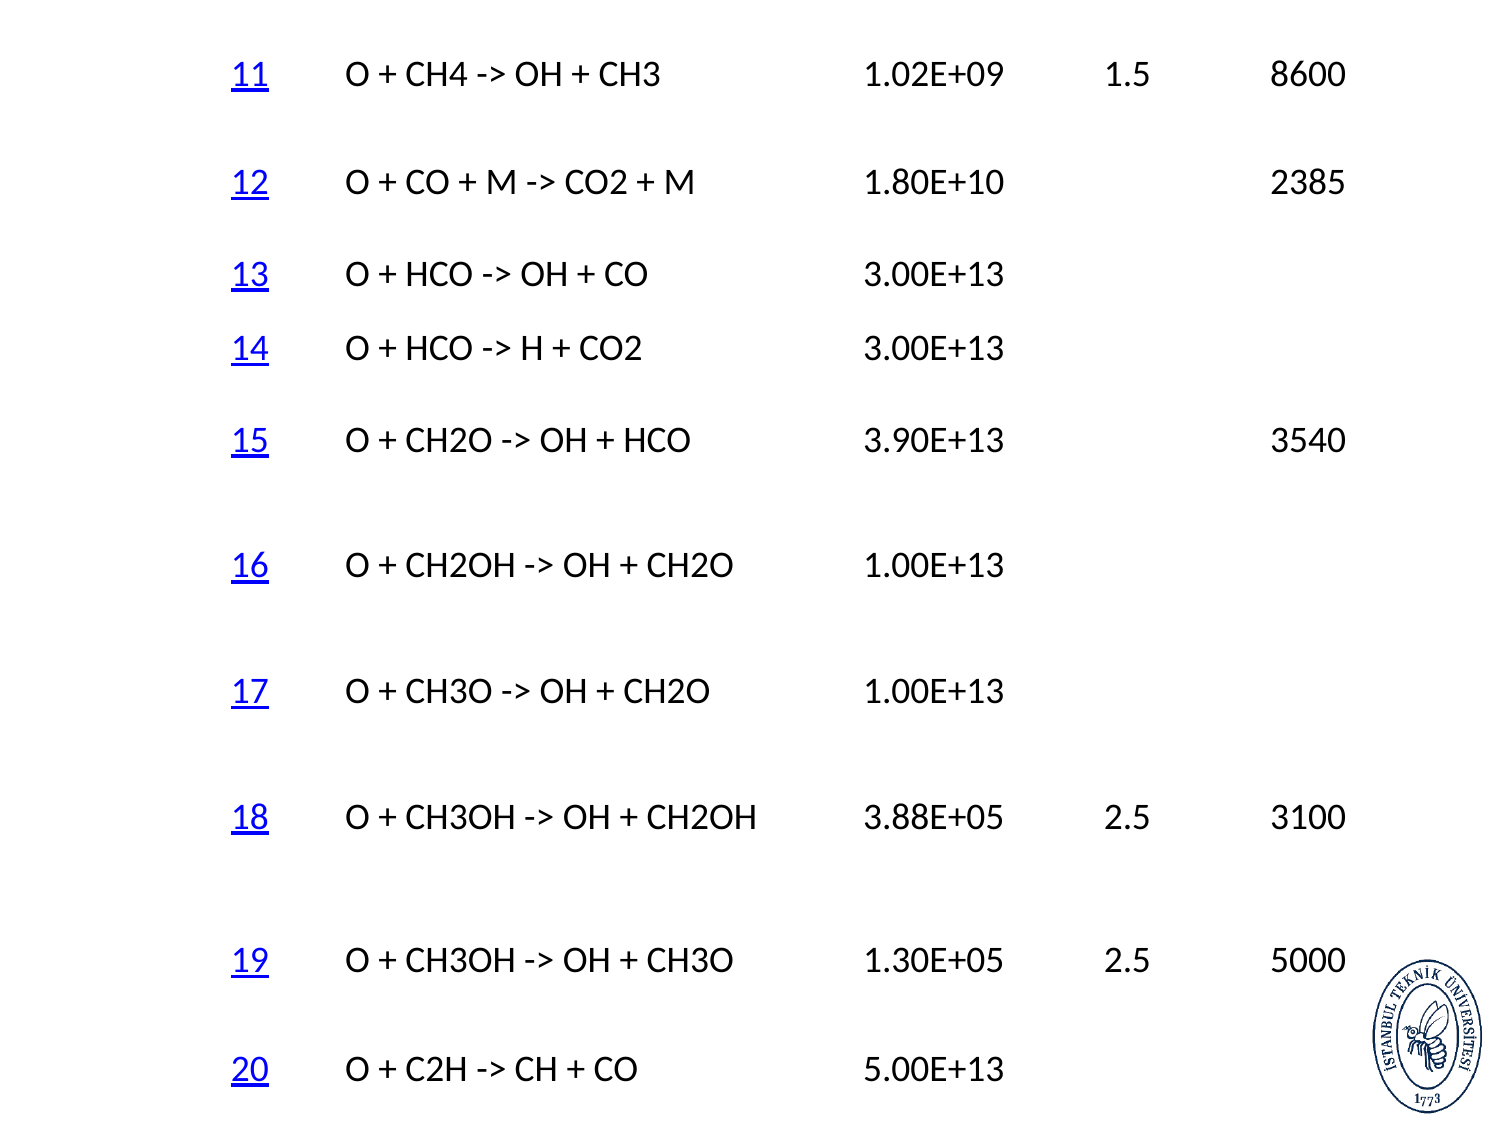
\includegraphics[width=0.95\linewidth,trim=10 40 10 40,clip]{slide61.png}
  \end{center}
\end{frame}

% =========================================================================
% Slide 62 -- GRI Mech 3.0 table 3
% =========================================================================
\begin{frame}{GRI--Mech 3.0 for Methane Combustion (3/4)}
  \begin{center}
    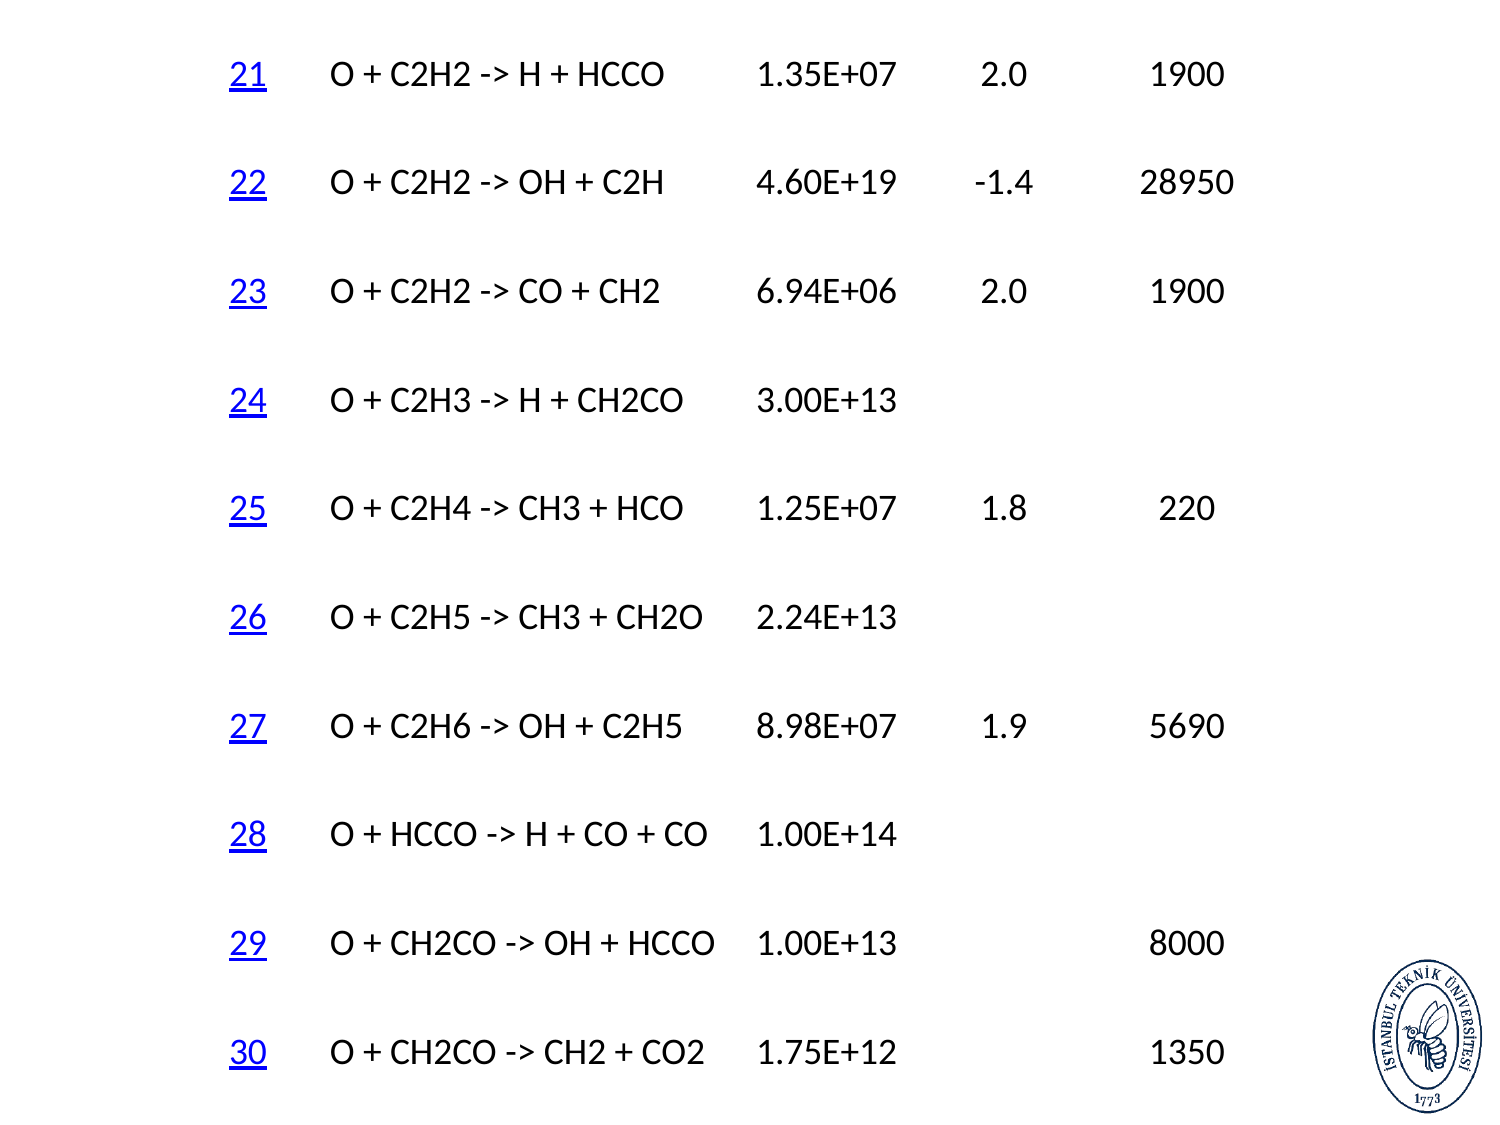
\includegraphics[width=0.95\linewidth,trim=10 40 10 40,clip]{slide62.png}
  \end{center}
\end{frame}

% =========================================================================
% Slide 63 -- GRI Mech 3.0 table 4
% =========================================================================
\begin{frame}{GRI--Mech 3.0 for Methane Combustion (4/4)}
  \begin{center}
    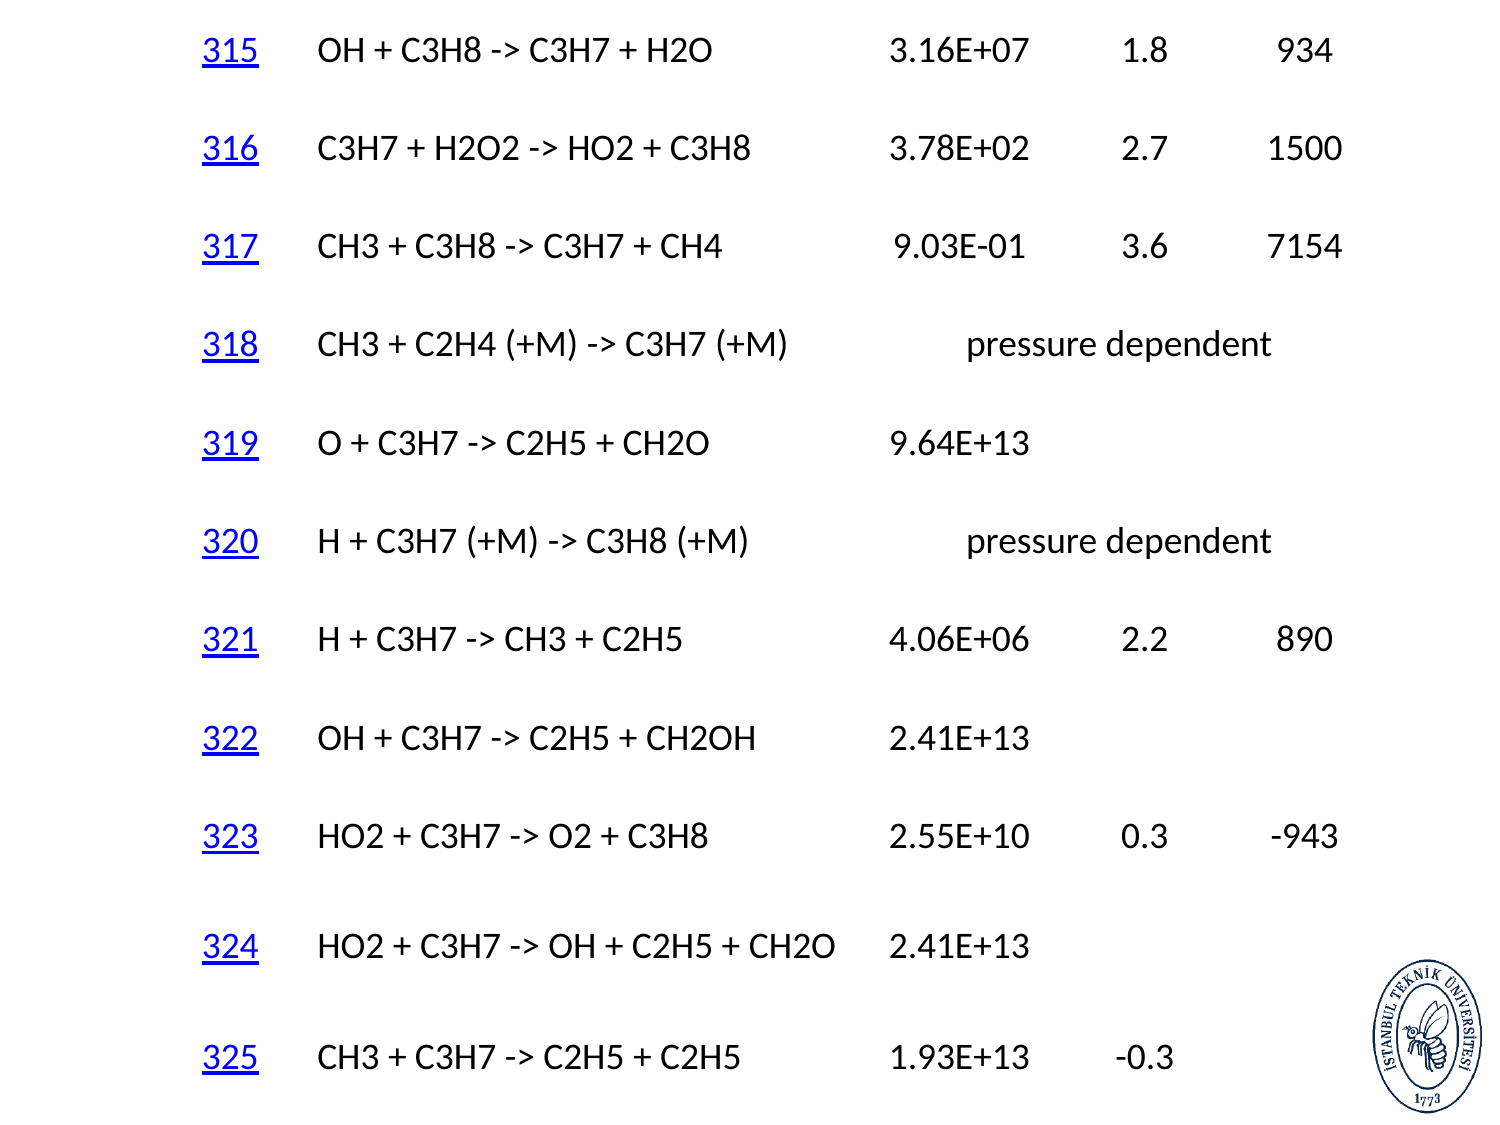
\includegraphics[width=0.95\linewidth,trim=10 40 10 40,clip]{slide63.png}
  \end{center}
\end{frame}

% =========================================================================
% Slide 64 -- Single rate detail
% =========================================================================
\begin{frame}{Detailed Rate: $\mathrm{O+O+M\rightarrow O_{2}+M}$}
  \begin{center}
    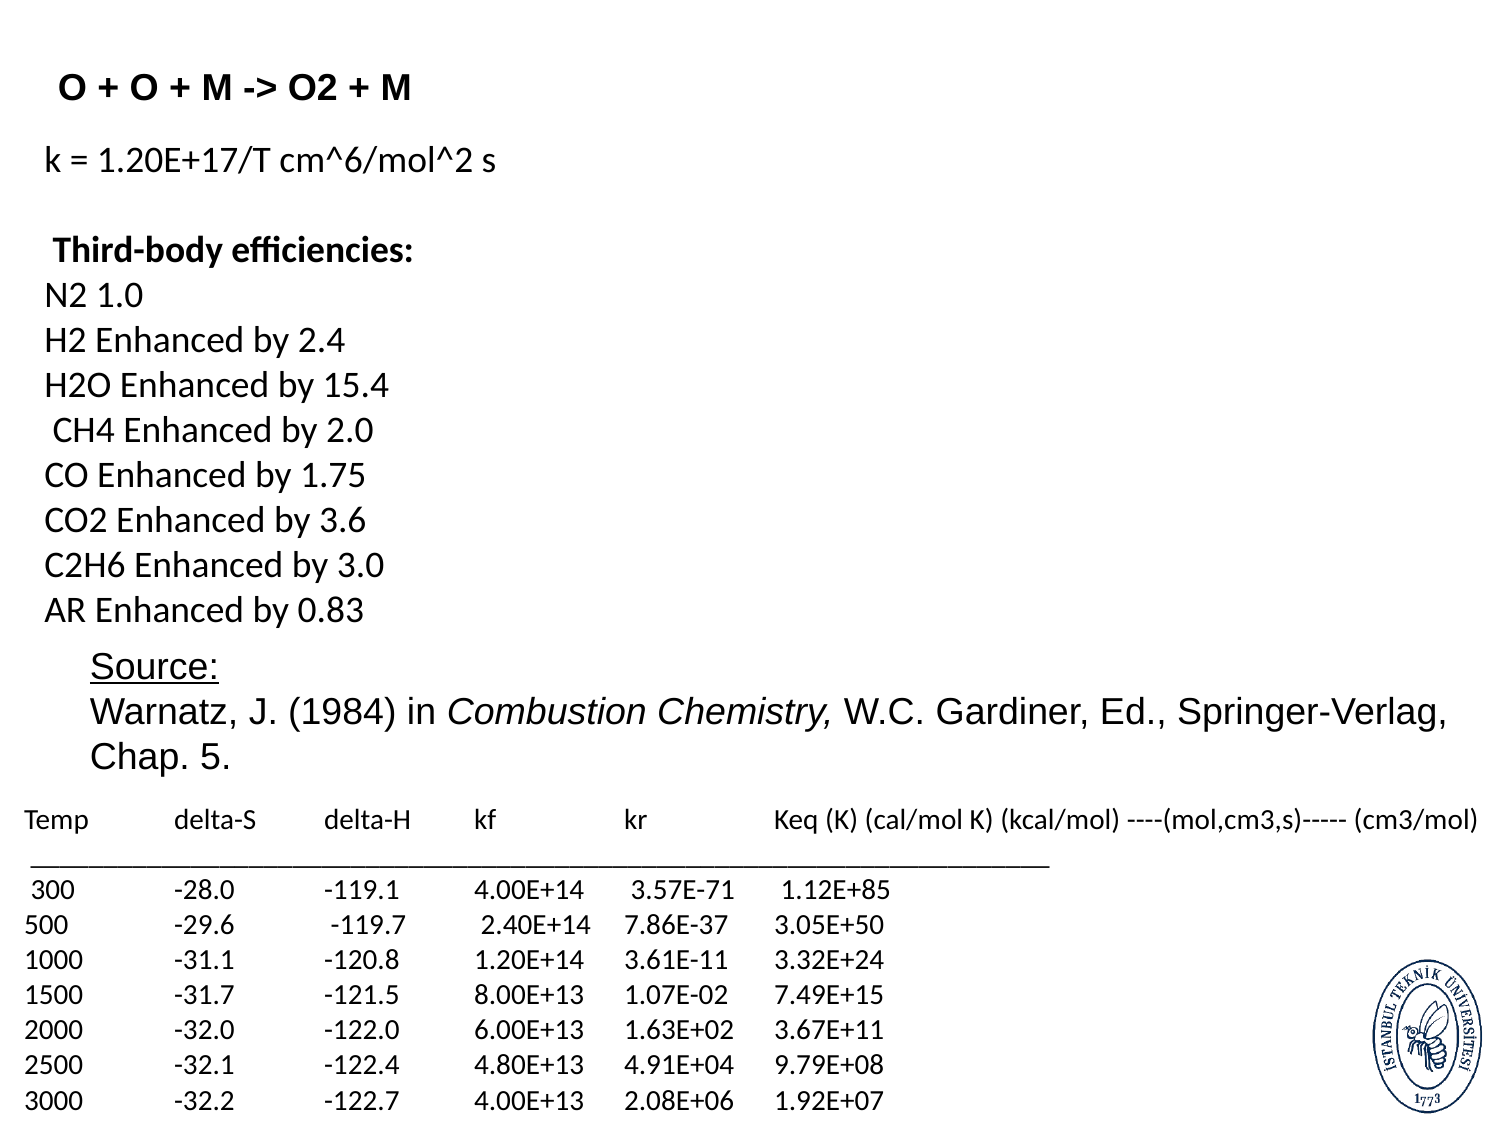
\includegraphics[width=0.85\linewidth,trim=10 40 10 40,clip]{slide64.png}
  \end{center}
\end{frame}

% =========================================================================
% Slide 65 -- CHEMKIN format
% =========================================================================
\begin{frame}{GRI--Mech 3.0 in CHEMKIN-II Format}
  \begin{center}
    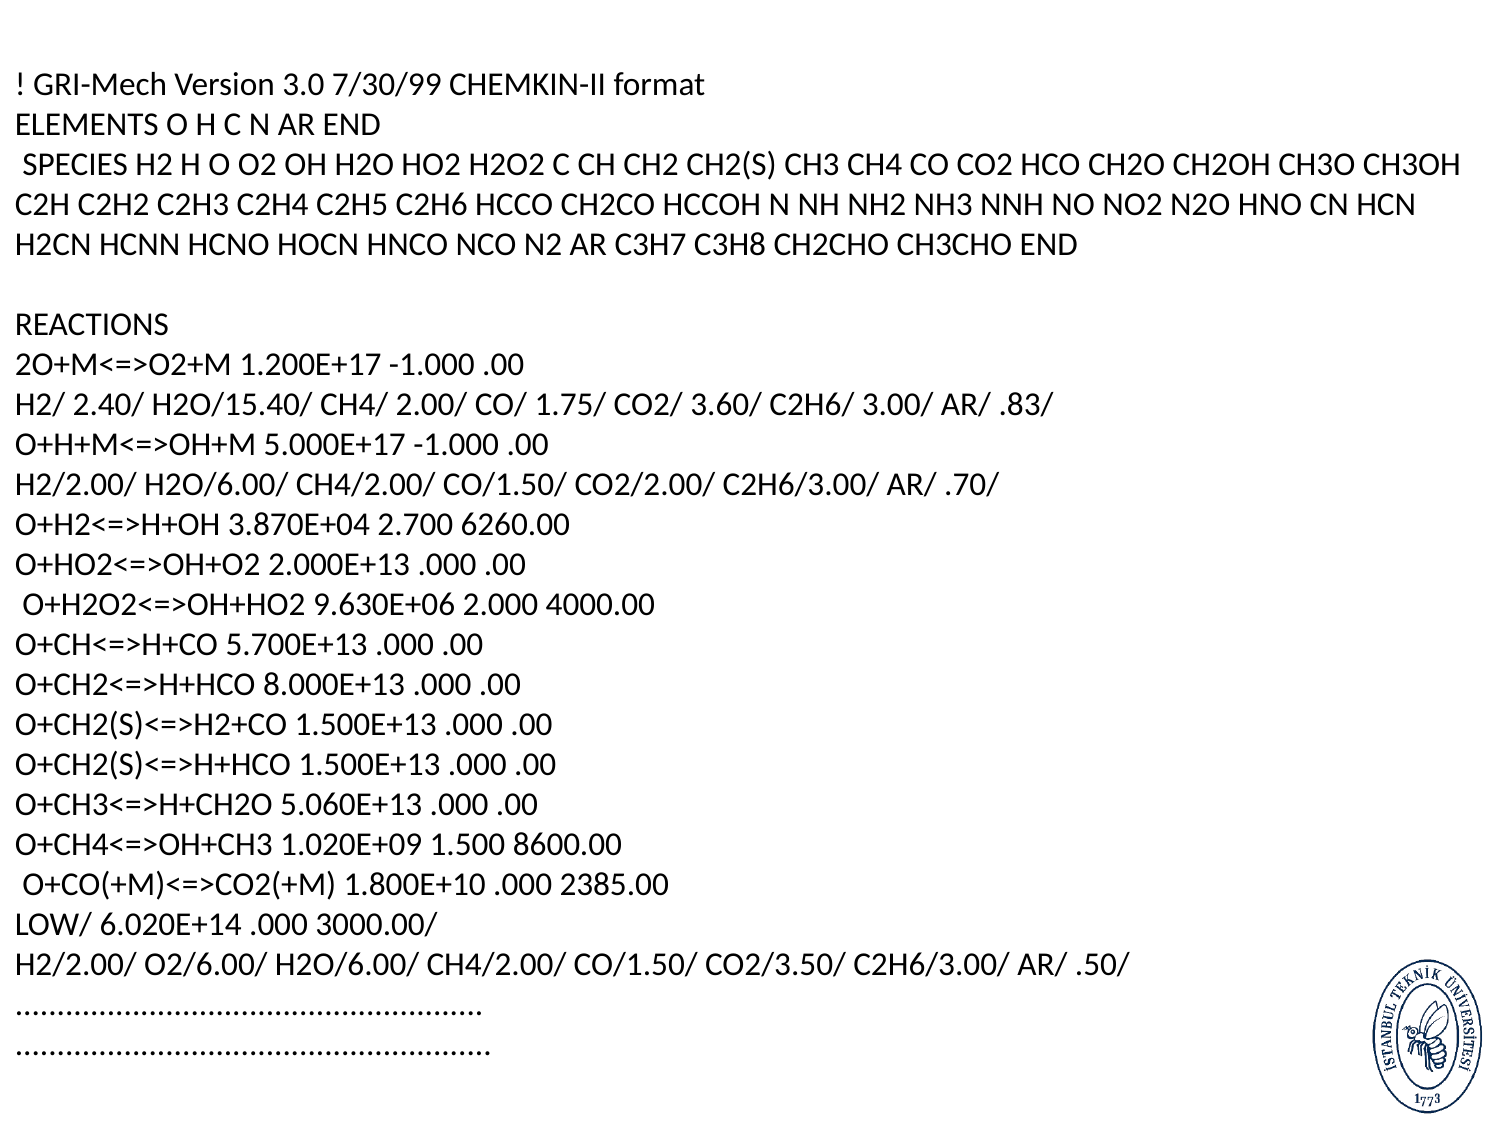
\includegraphics[width=0.95\linewidth,trim=10 40 10 40,clip]{slide65.png}
  \end{center}
\end{frame}

% =========================================================================
% Slide 66 -- Shomate equation
% =========================================================================
\begin{frame}{Gas-Phase Heat Capacity (Shomate Equation)}
  \begin{center}
    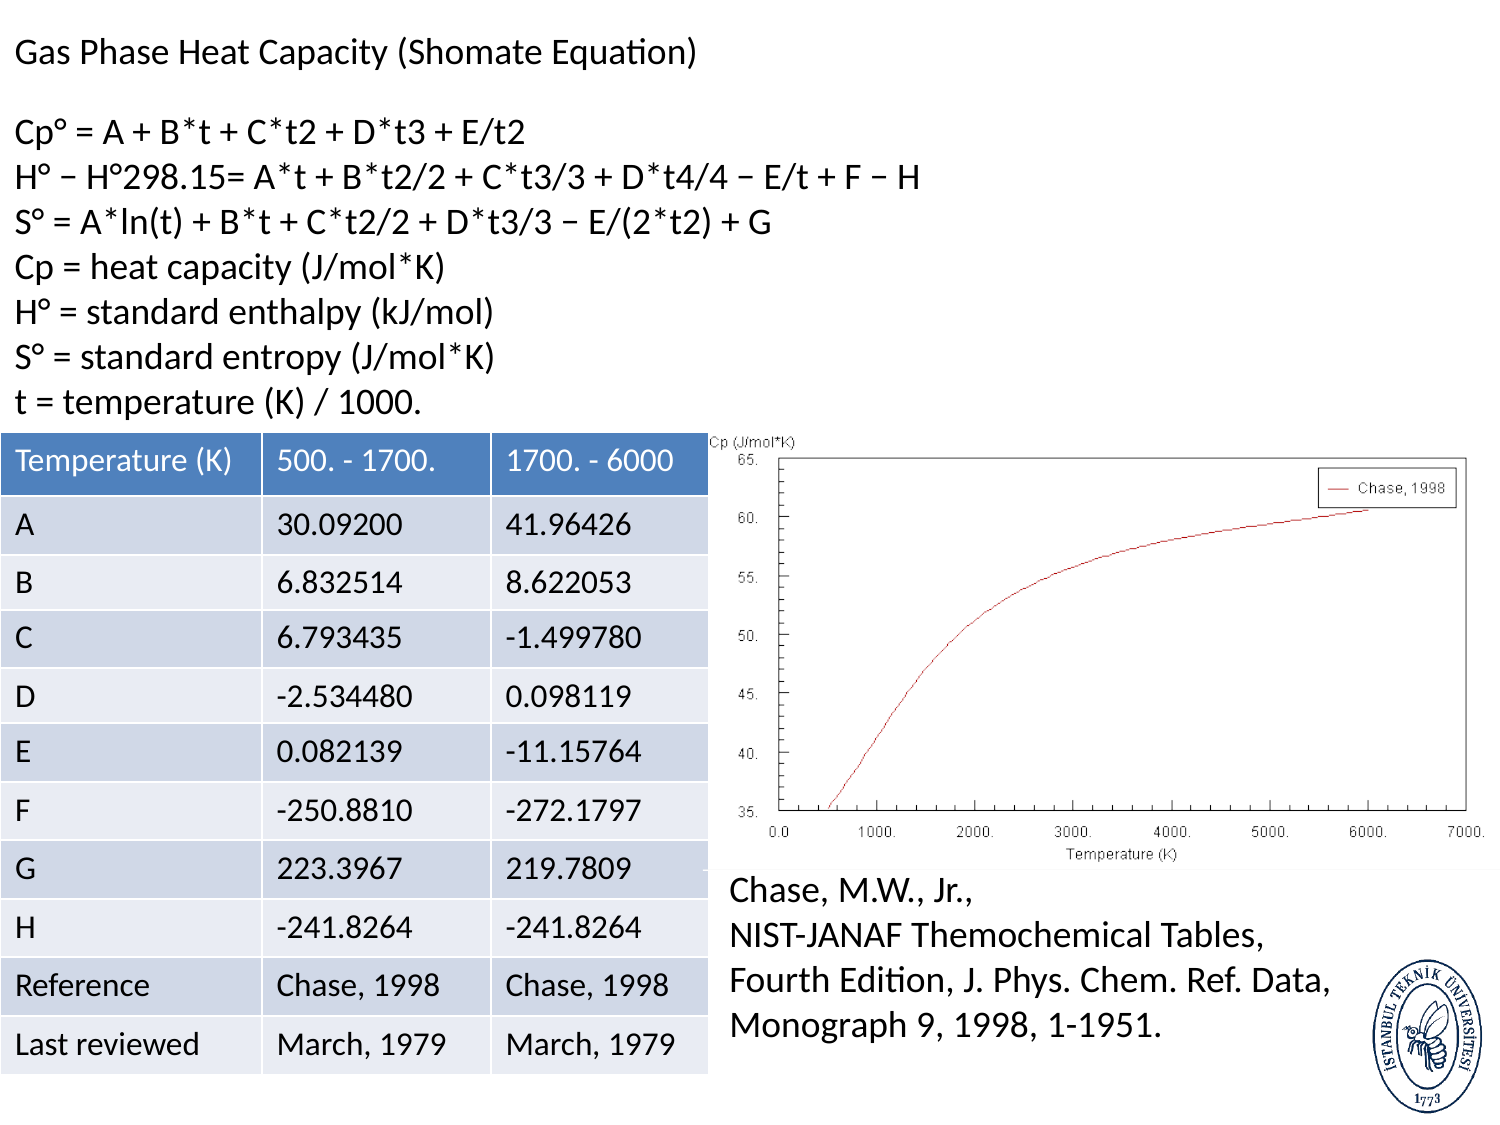
\includegraphics[width=0.95\linewidth,trim=10 40 10 40,clip]{slide66.png}
  \end{center}
\end{frame}

% =========================================================================
% Slide 67 -- NASA polynomial format
% =========================================================================
\begin{frame}{NASA Polynomial Format for CHEMKIN-II}
  \begin{center}
    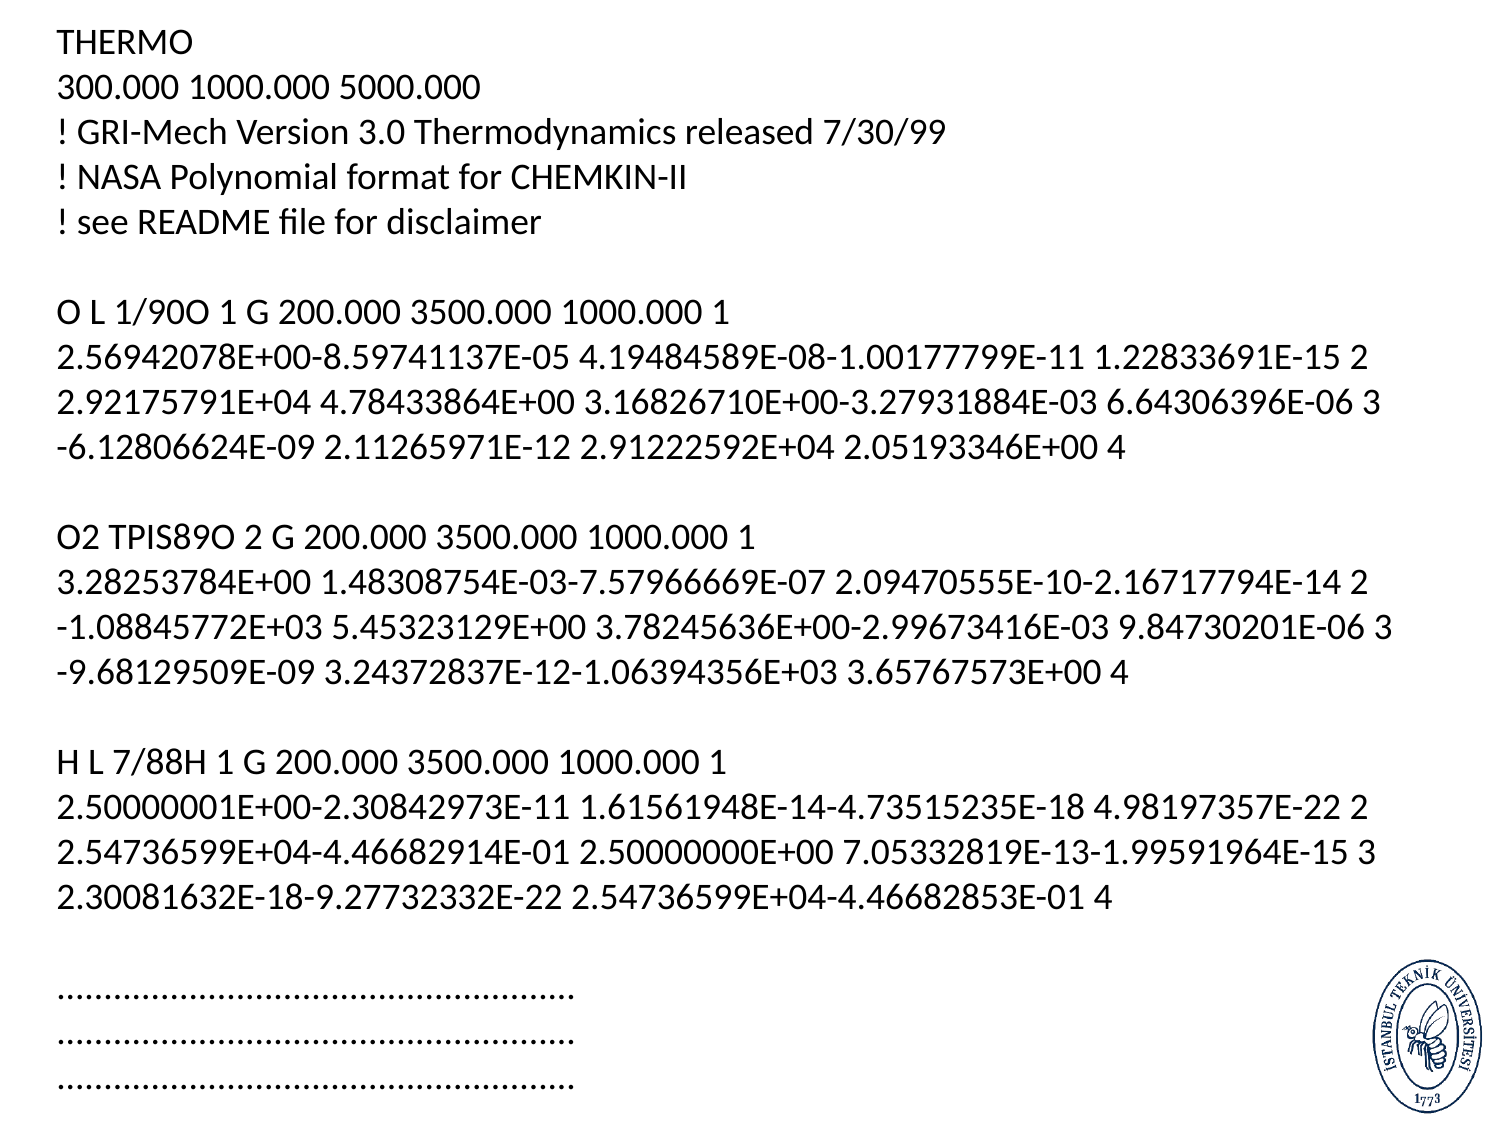
\includegraphics[width=0.95\linewidth,trim=10 40 10 40,clip]{slide67.png}
  \end{center}
\end{frame}

% =========================================================================
% Slide 68 -- Ignition delay benchmark
% =========================================================================
\begin{frame}{Mechanism Validation: Ignition Delay}
  \begin{center}
    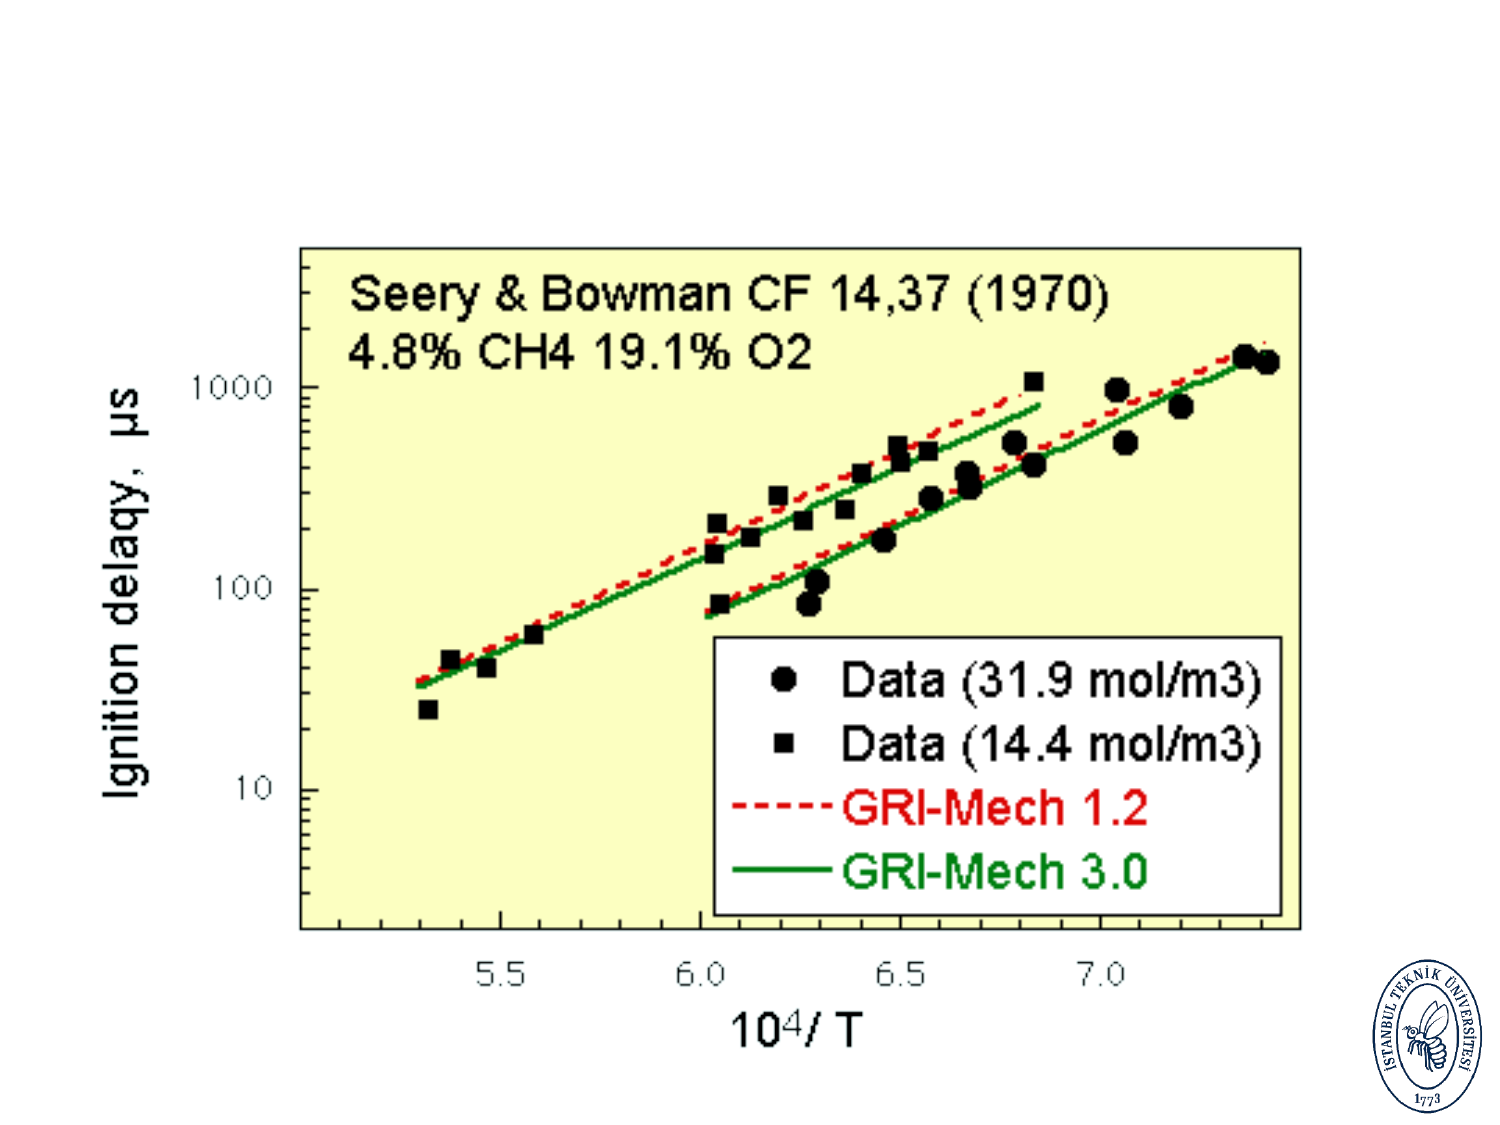
\includegraphics[width=0.85\linewidth,trim=10 40 10 40,clip]{slide68.png}
  \end{center}
\end{frame}

% =========================================================================
% Slide 69 -- Flame velocity vs pressure
% =========================================================================
\begin{frame}{Mechanism Validation: Flame Velocity vs.\ Pressure}
  \begin{center}
    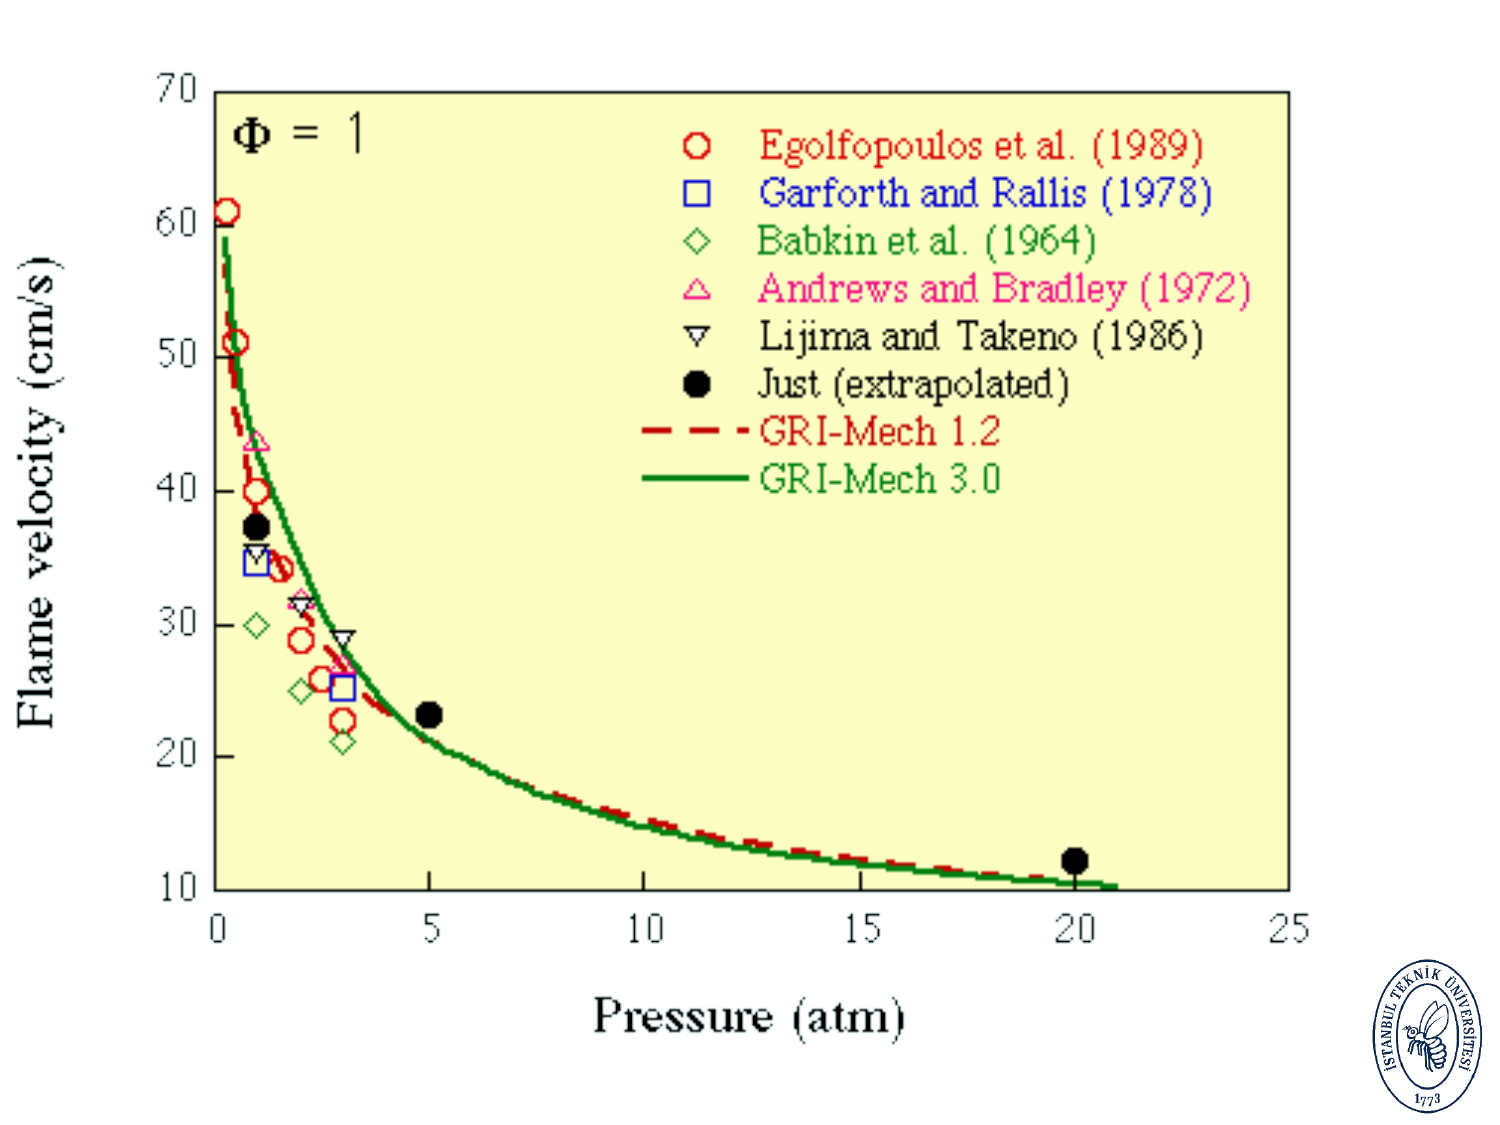
\includegraphics[width=0.85\linewidth,trim=10 40 10 40,clip]{slide69.png}
  \end{center}
\end{frame}

% =========================================================================
% Slide 70 -- OH benchmark
% =========================================================================
\begin{frame}{Mechanism Validation: OH Time History}
  \begin{center}
    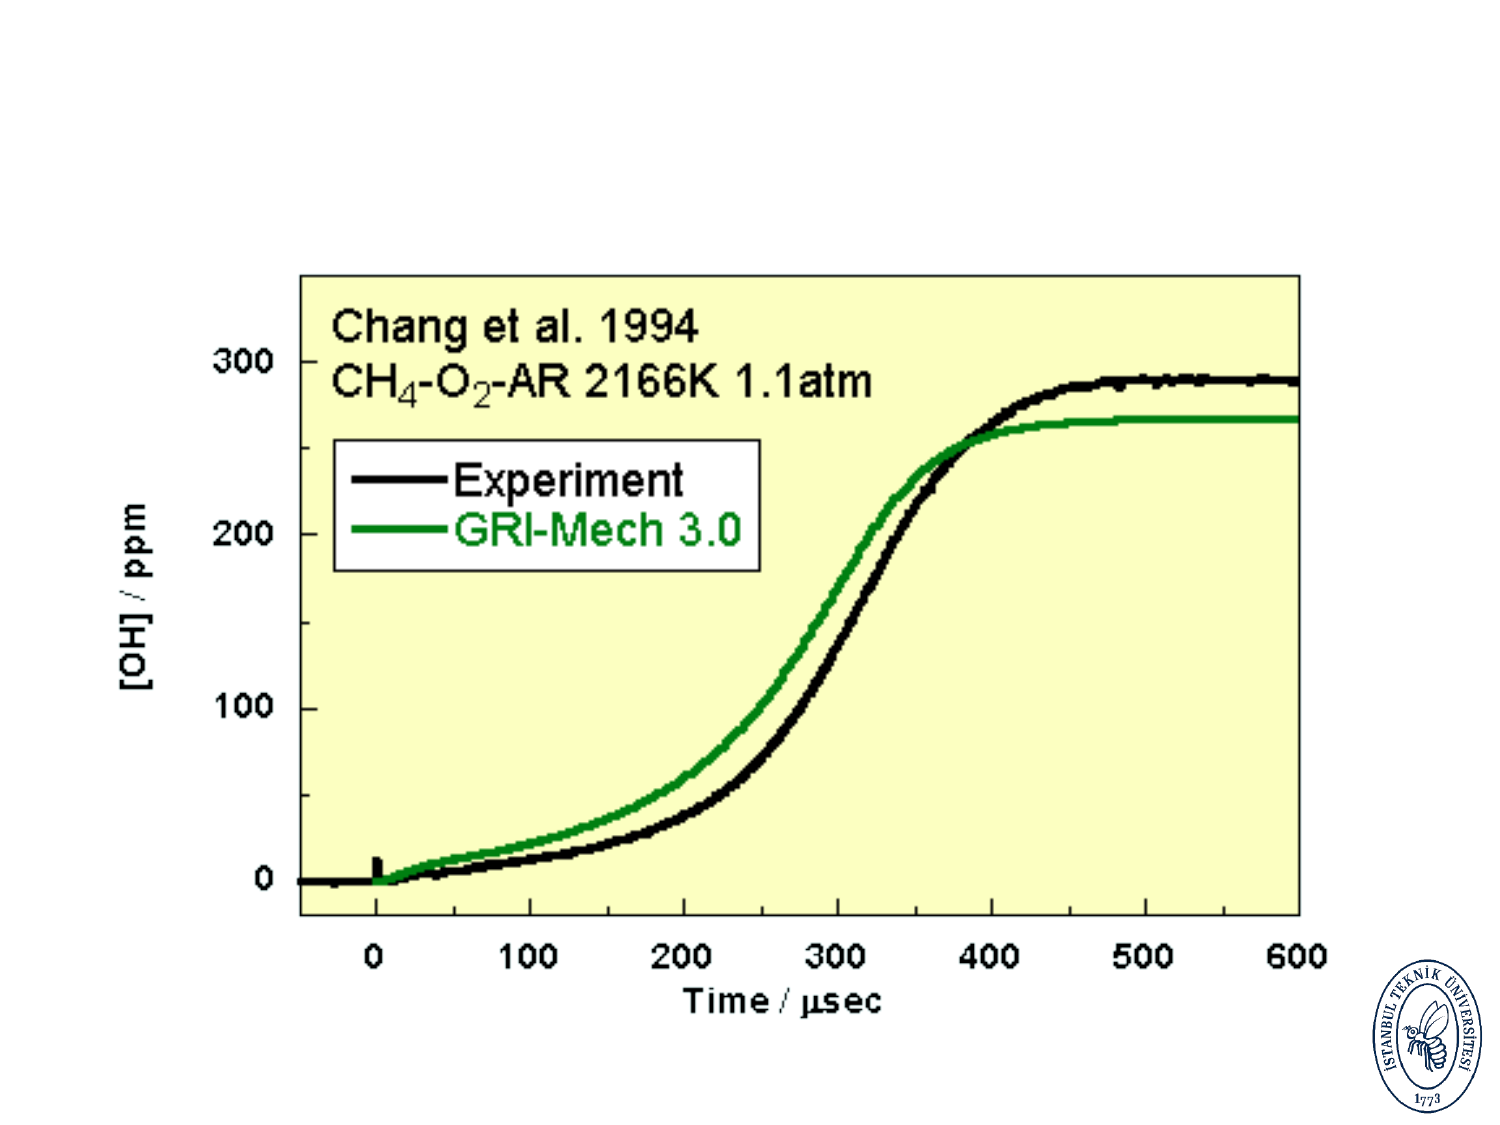
\includegraphics[width=0.85\linewidth,trim=10 40 10 40,clip]{slide70.png}
  \end{center}
\end{frame}

% =========================================================================
% Slide 71 -- CO2 benchmark
% =========================================================================
\begin{frame}{Mechanism Validation: CO$_{2}$ in CH$_{4}$ Wet Reactor}
  \begin{center}
    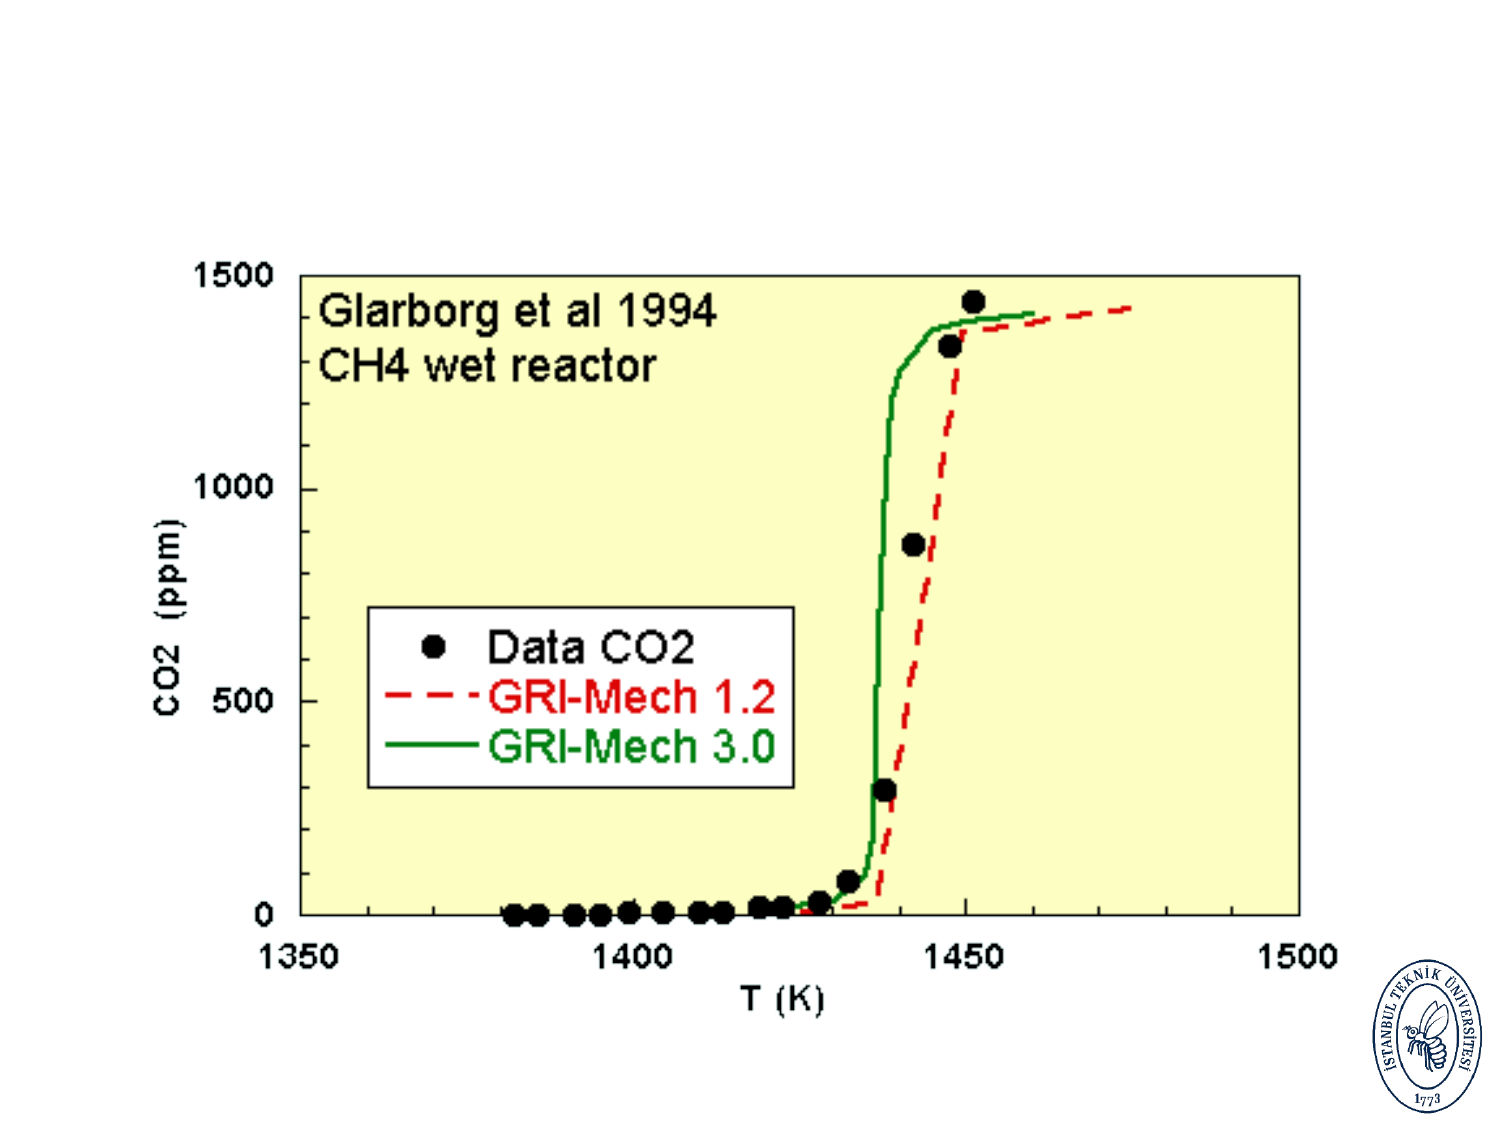
\includegraphics[width=0.85\linewidth,trim=10 40 10 40,clip]{slide71.png}
  \end{center}
\end{frame}

% =========================================================================
% Slide 72 -- Case Study I title
% =========================================================================
\begin{frame}[plain]
  \vfill
  \begin{center}
    {\Large\bfseries Case Study --- I}\\[8pt]
    {\large Calculation of Laminar Flame Speeds of Methane/Hydrogen Mixtures}
  \end{center}
  \vfill
\end{frame}

% =========================================================================
% Slide 73 -- Equivalence ratio for CH4/H2
% =========================================================================
\begin{frame}{Equivalence Ratio for CH$_{4}$/H$_{2}$ Mixtures}
  \[
    \phi \;=\; \frac{C_{CH_{4}}/\bigl[C_{HAVA} - C_{H_{2}}/(C_{H_{2}}/C_{HAVA})_{st}\bigr]}{(C_{CH_{4}}/C_{HAVA})_{st}}
  \]
\end{frame}

% =========================================================================
% Slide 74 -- Governing equations for 1D flame
% =========================================================================
\begin{frame}{Governing Equations}
  \begin{block}{Species conservation}
    \[
      \pd{(\rho Y_{i})}{t} + \pd{(\rho u Y_{i})}{x}
        \;=\; \pd{}{x}\!\Bigl(\rho \mathcal{D}\,\pd{Y_{i}}{x}\Bigr) + \dot{w}_{i}
    \]
  \end{block}
  \begin{block}{Conservation of energy}
    \[
      \rho c_{p}\!\left[\pd{T}{t} + u\,\pd{T}{x}\right]
        \;=\; -\sum_{k=1}^{N}\!h_{k}\dot{w}_{k}
              + \pd{}{x}\!\Bigl(\lambda\,\pd{T}{x}\Bigr)
              - \rho\,\pd{T}{x}\!\Bigl(\sum_{k}c_{p,k}Y_{k}U_{k}\Bigr)
    \]
  \end{block}
  \begin{block}{Momentum equation}
    \[
      u\,\frac{\dd u}{\dd x} \;=\; -\frac{1}{\rho}\,\frac{\dd P}{\dd x}
    \]
  \end{block}
\end{frame}

% =========================================================================
% Slide 75 -- 1D grid
% =========================================================================
\begin{frame}{Computational Domain (1D)}
  \begin{center}
    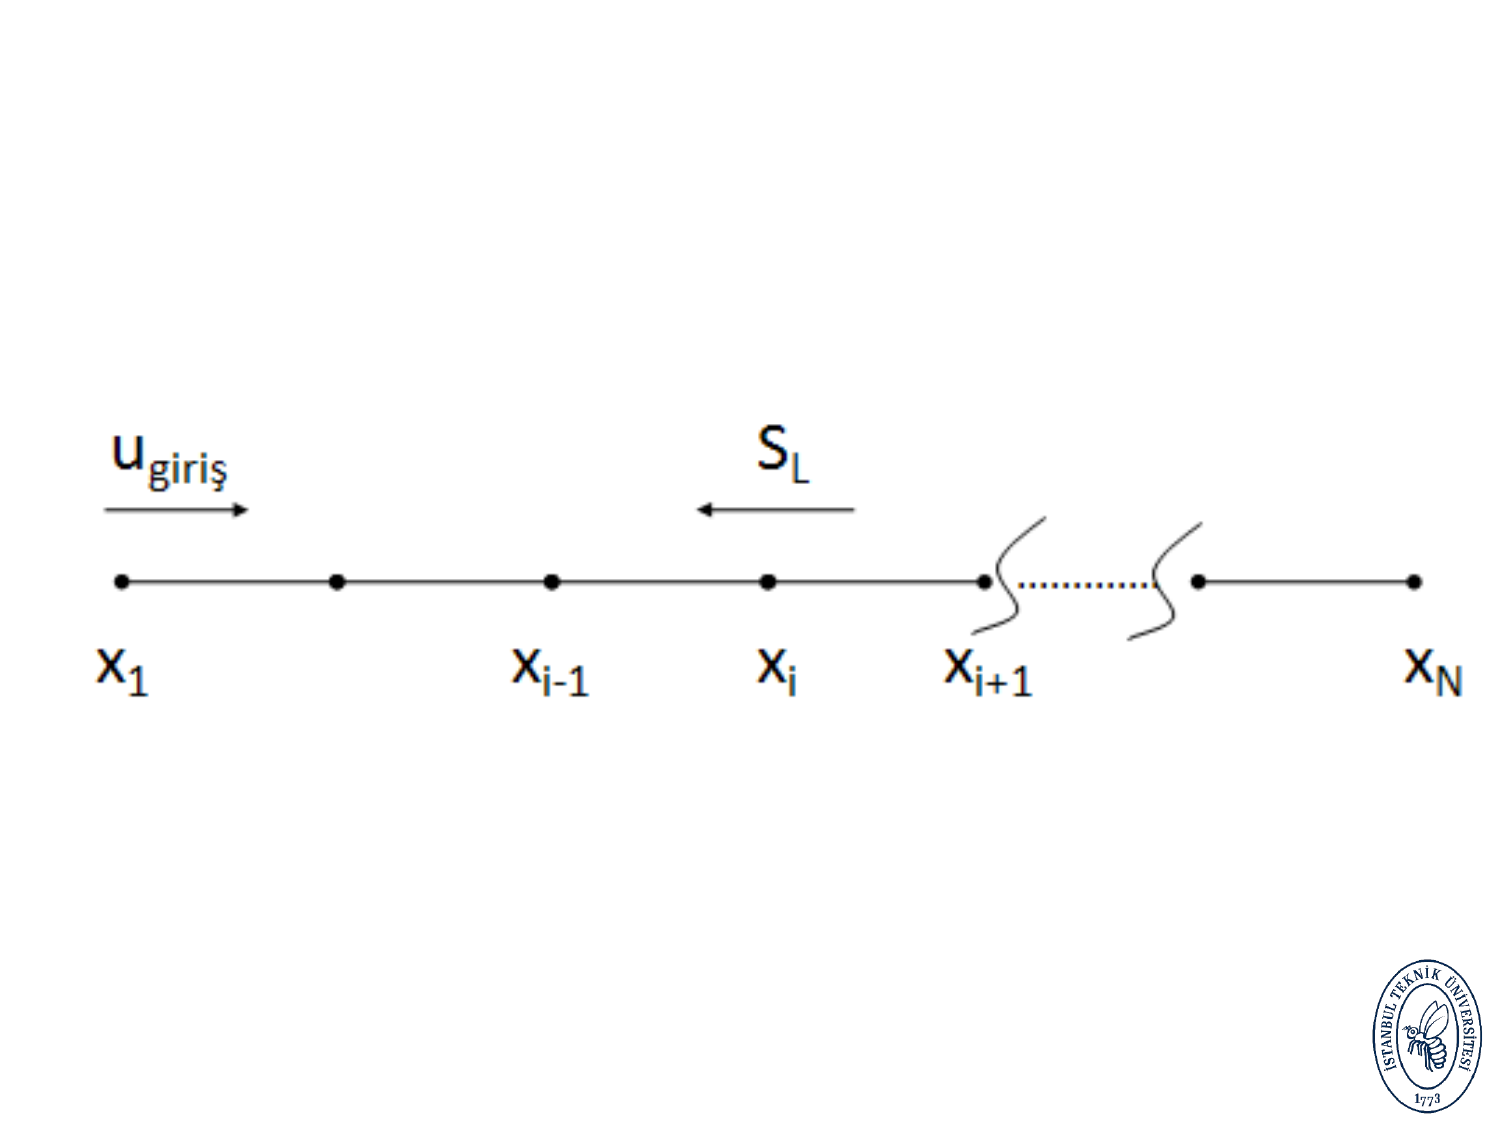
\includegraphics[width=0.8\linewidth,trim=10 40 10 60,clip]{slide75.png}
  \end{center}
\end{frame}

% =========================================================================
% Slide 76 -- Species/temperature profile
% =========================================================================
\begin{frame}{Flame Structure ($\phi=1$, 70\% CH$_{4}$ -- 30\% H$_{2}$)}
  \begin{center}
    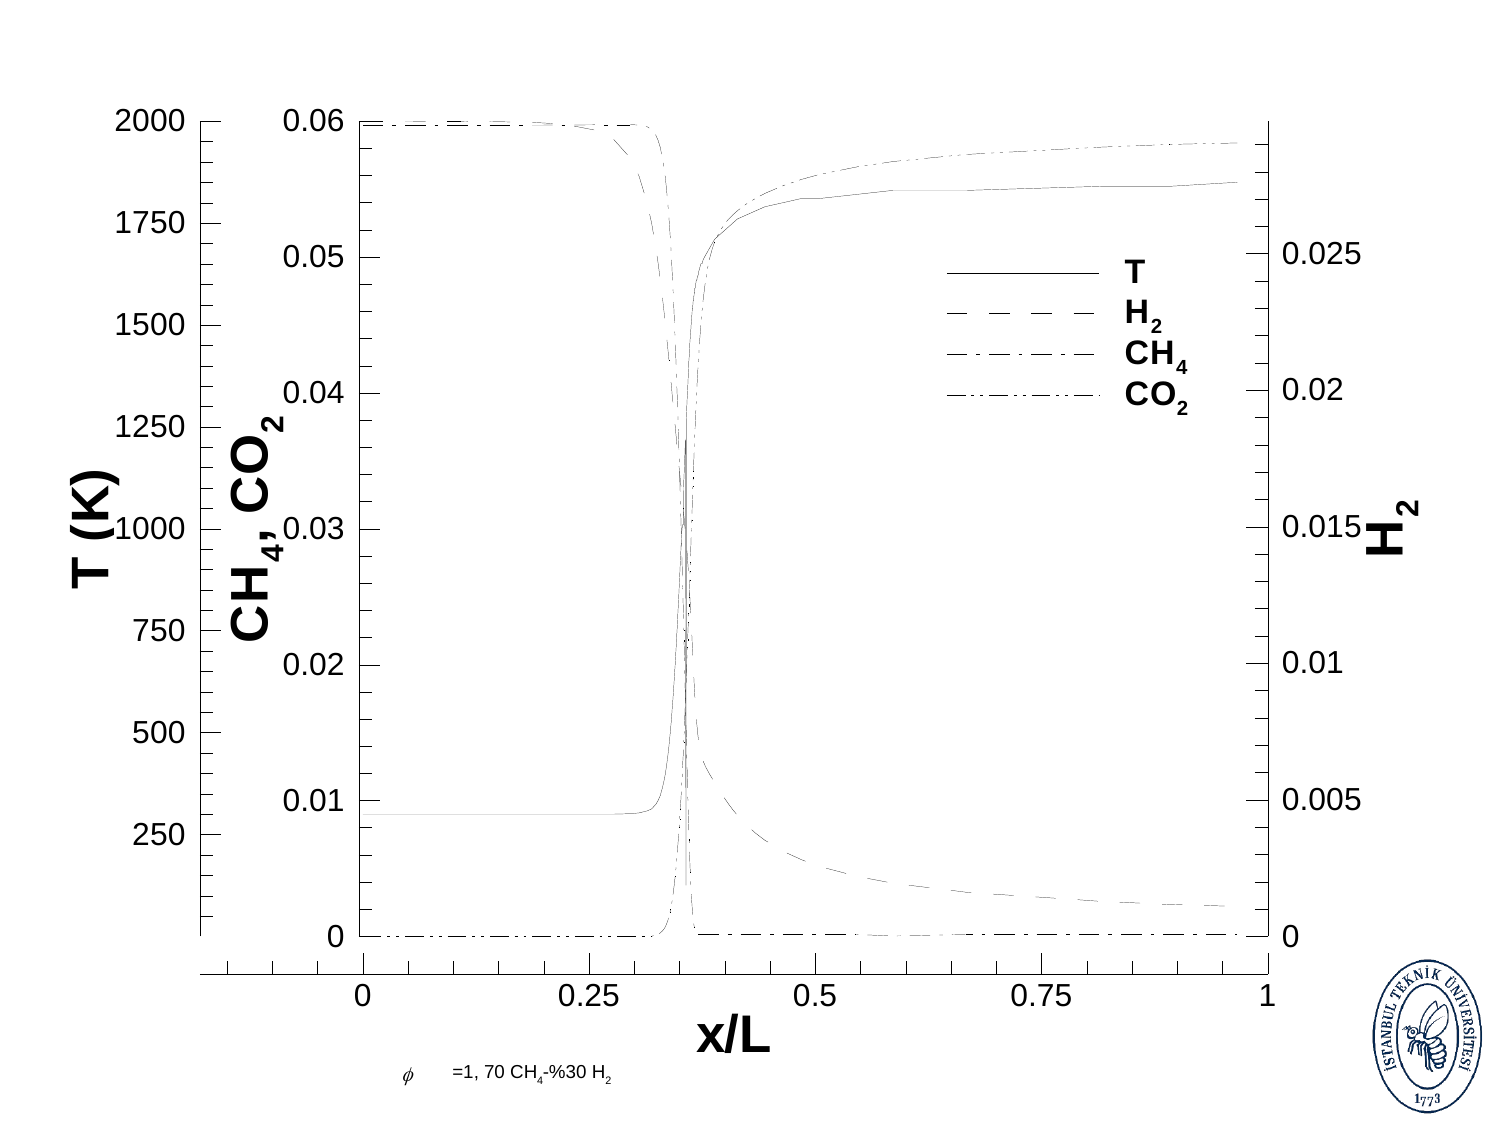
\includegraphics[width=0.8\linewidth,trim=10 40 10 40,clip]{slide76.png}
  \end{center}
\end{frame}

% =========================================================================
% Slide 77 -- OH reaction path diagram
% =========================================================================
\begin{frame}{Reaction Path Diagram: OH}
  \begin{center}
    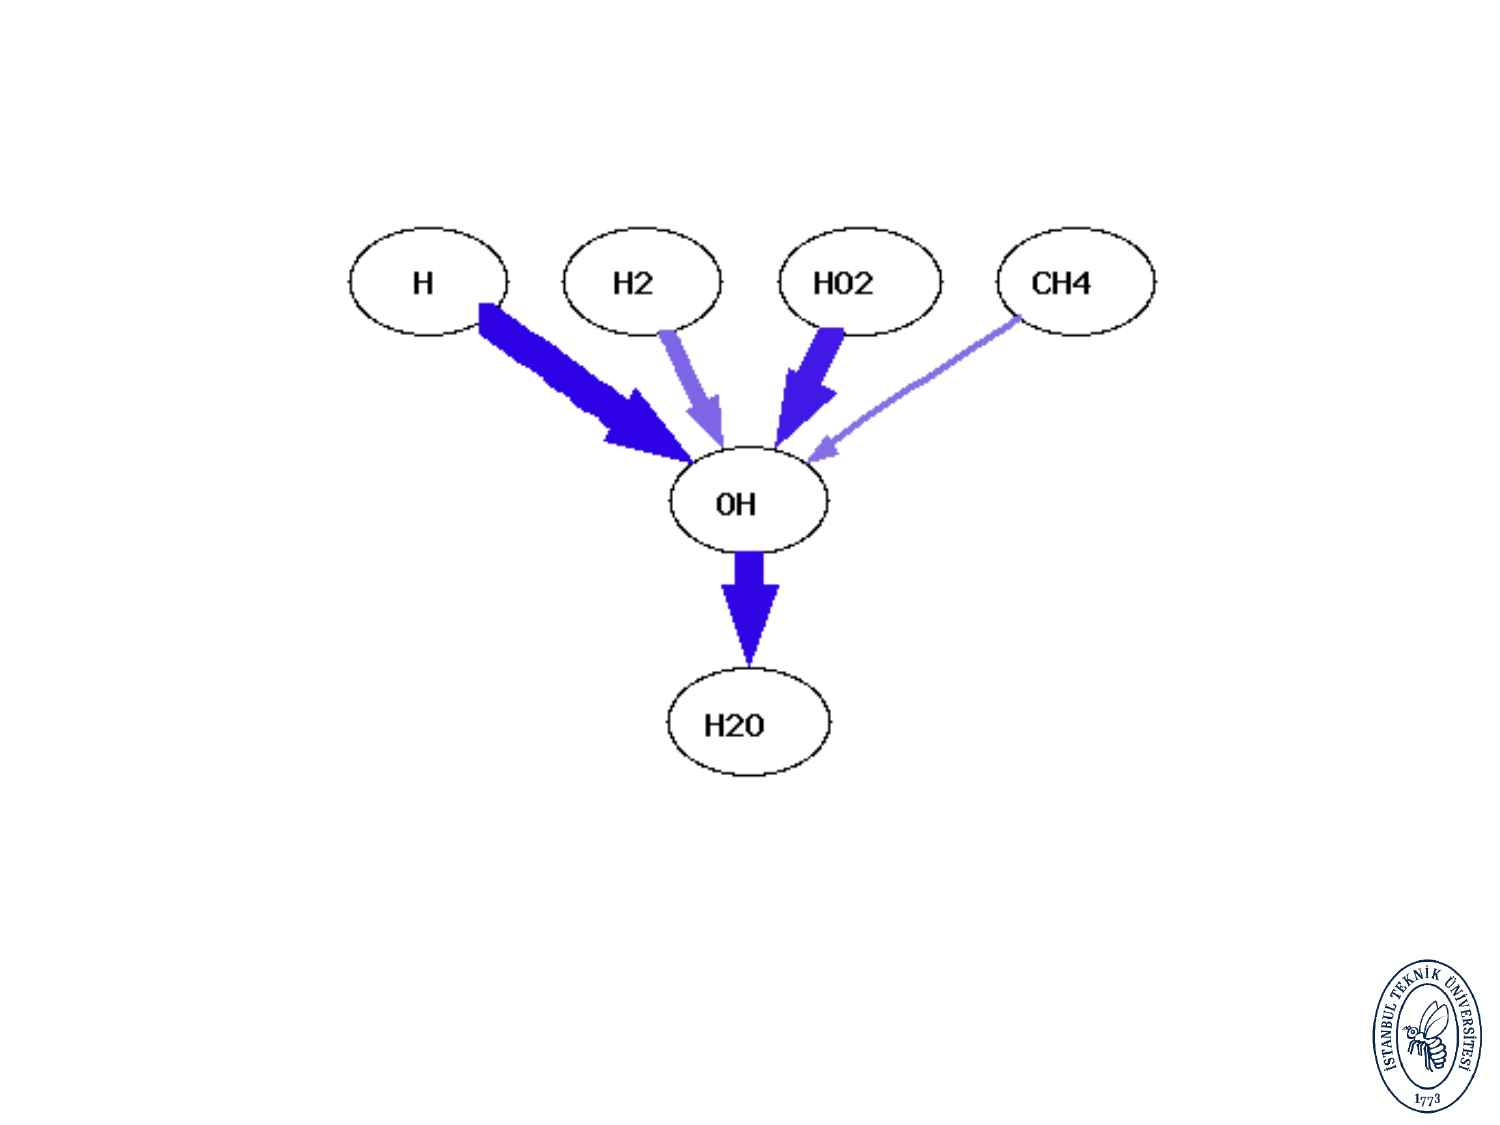
\includegraphics[width=0.8\linewidth,trim=10 40 10 40,clip]{slide77.png}
  \end{center}
\end{frame}

% =========================================================================
% Slide 78 -- CH4 reaction path diagram
% =========================================================================
\begin{frame}{Reaction Path Diagram: CH$_{4}$}
  \begin{center}
    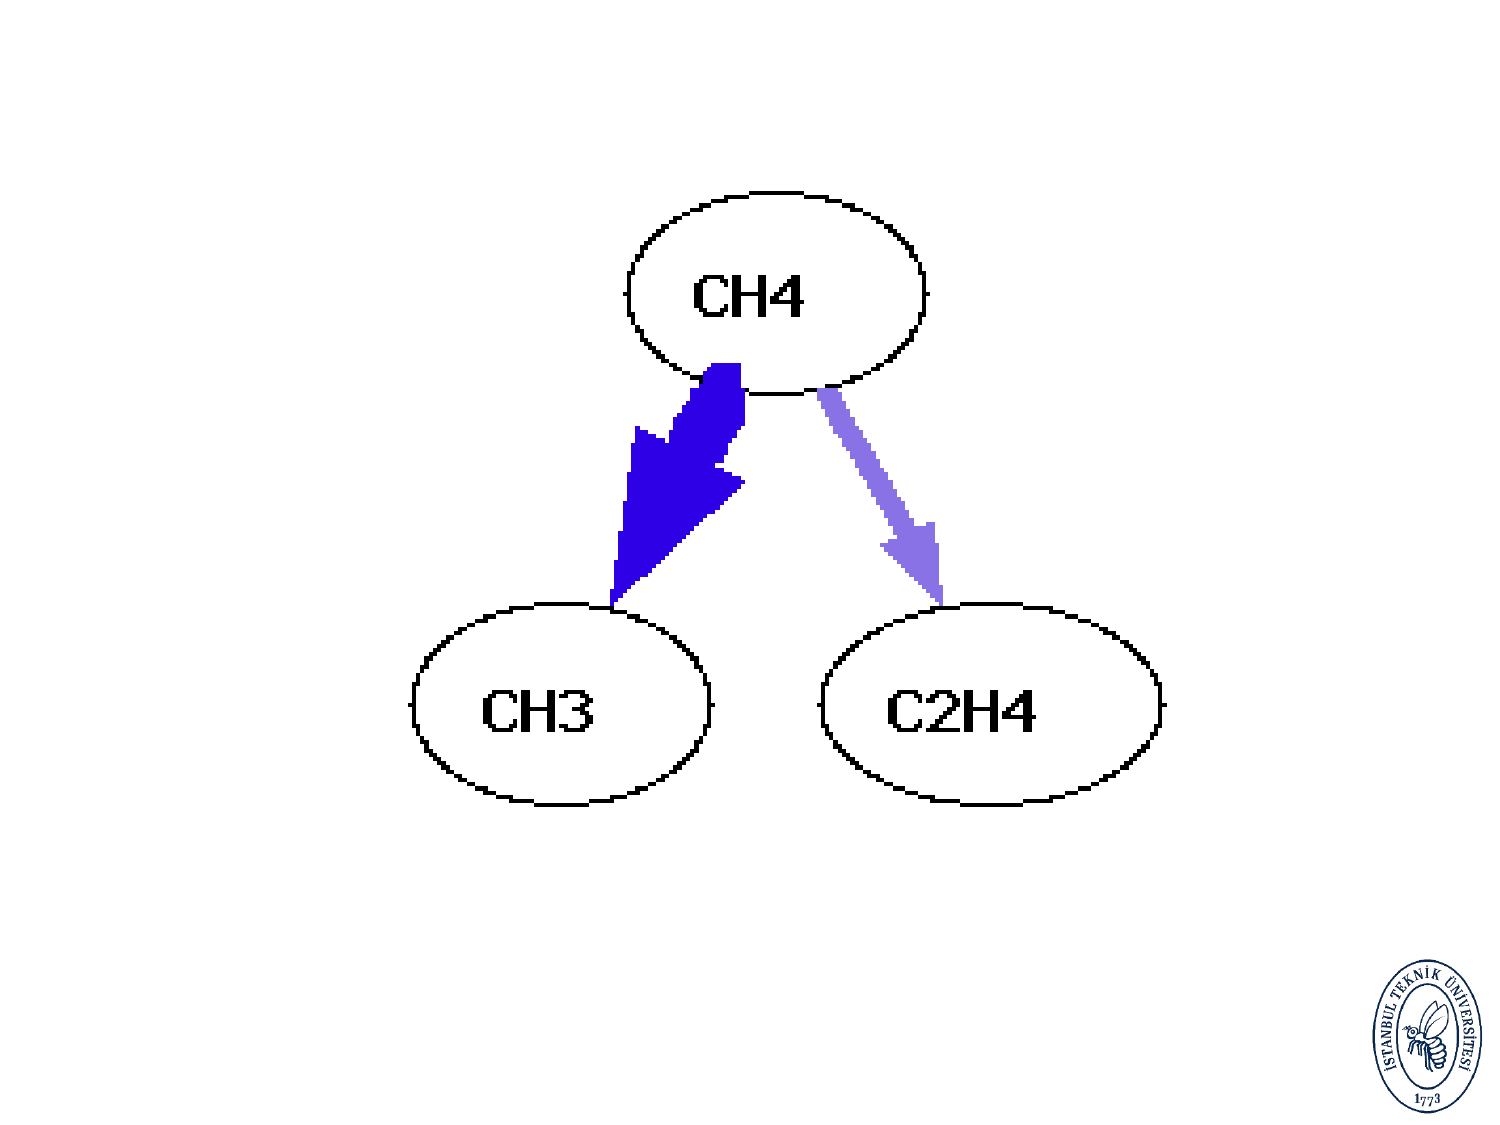
\includegraphics[width=0.8\linewidth,trim=10 40 10 40,clip]{slide78.png}
  \end{center}
\end{frame}

% =========================================================================
% Slide 79 -- Adiabatic flame temperature vs phi
% =========================================================================
\begin{frame}{Adiabatic Flame Temperature vs.\ $\phi$}
  \begin{center}
    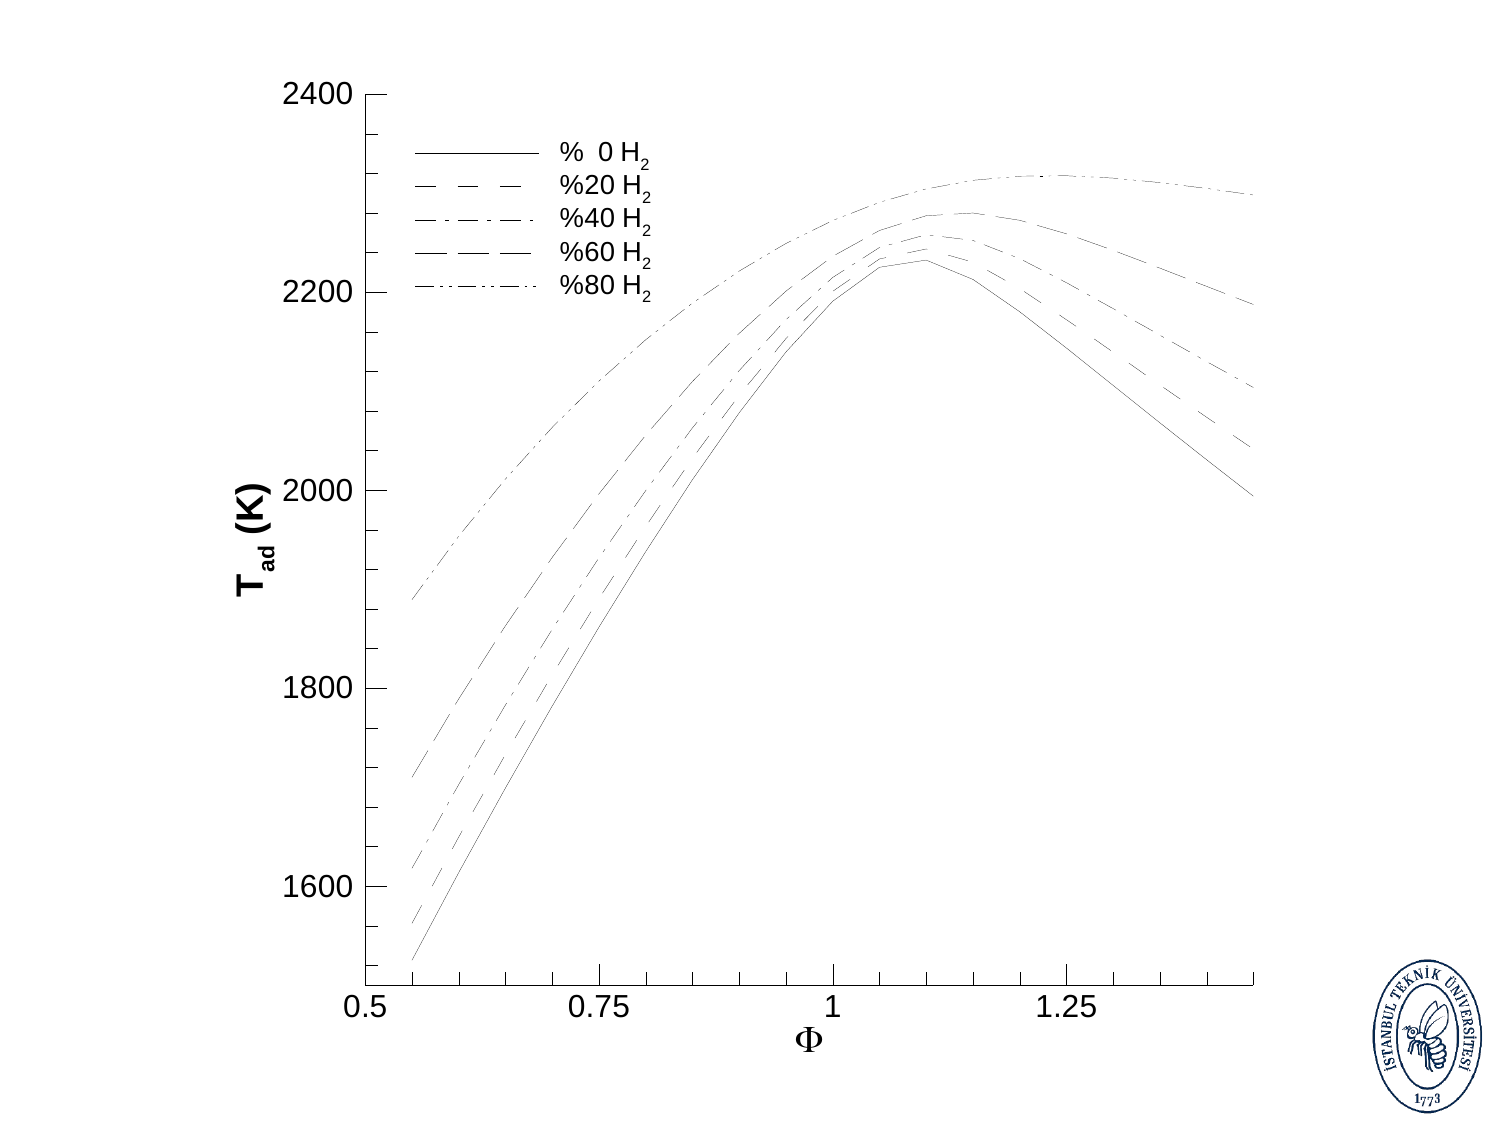
\includegraphics[width=0.85\linewidth,trim=10 40 10 40,clip]{slide79.png}
  \end{center}
\end{frame}

% =========================================================================
% Slide 80 -- Correlation for SL
% =========================================================================
\begin{frame}{Correlation for the Laminar Flame Speed}
  \[
    \frac{S_{L}}{S_{L,\mathrm{st}}}
      \;=\; \exp\!\left[\!\left(\frac{T_{ad} - T_{ad,\mathrm{st}}}{T_{ad}}\right)^{4}\right]
  \]
  \[
    \frac{S_{L,\mathrm{st}} - S_{L,\mathrm{st},CH_{4}}}{S_{L,\mathrm{st},H_{2}} - S_{L,\mathrm{st},CH_{4}}}
      \;=\; \!\left(\frac{T_{ad,\mathrm{st}} - T_{ad,\mathrm{st},CH_{4}}}{T_{ad,\mathrm{st},H_{2}} - T_{ad,\mathrm{st},CH_{4}}}\right)^{1.4 + n\alpha}
  \]
  \begin{tabular}{ll}
    $P=1$~atm, & $n=0.15$ \\
    $P=2$~atm, & $n=0.5$ \\
    $P=3$~atm, & $n=0.8$
  \end{tabular}
  \resizebox{\linewidth}{!}{$\displaystyle
    S_{L} \;=\; \!\left[(S_{L,\mathrm{st},H_{2}} - S_{L,\mathrm{st},CH_{4}})
                        \!\left(\frac{T_{ad,\mathrm{st}} - T_{ad,\mathrm{st},CH_{4}}}{T_{ad,\mathrm{st},H_{2}} - T_{ad,\mathrm{st},CH_{4}}}\right)^{1.4 + n\alpha}
                        + S_{L,\mathrm{st},CH_{4}}\right]
                \exp\!\left[\!\left(\tfrac{T_{ad} - T_{ad,\mathrm{st}}}{T_{ad}}\right)^{4}\right]
  $}
  \par\medskip
  \footnotesize $\alpha$ denotes the volumetric fraction of hydrogen.
\end{frame}

% =========================================================================
% Slide 81 -- SL vs phi P=1 atm
% =========================================================================
\begin{frame}{Laminar Flame Speed vs.\ $\phi$ ($P=1$ atm)}
  \begin{center}
    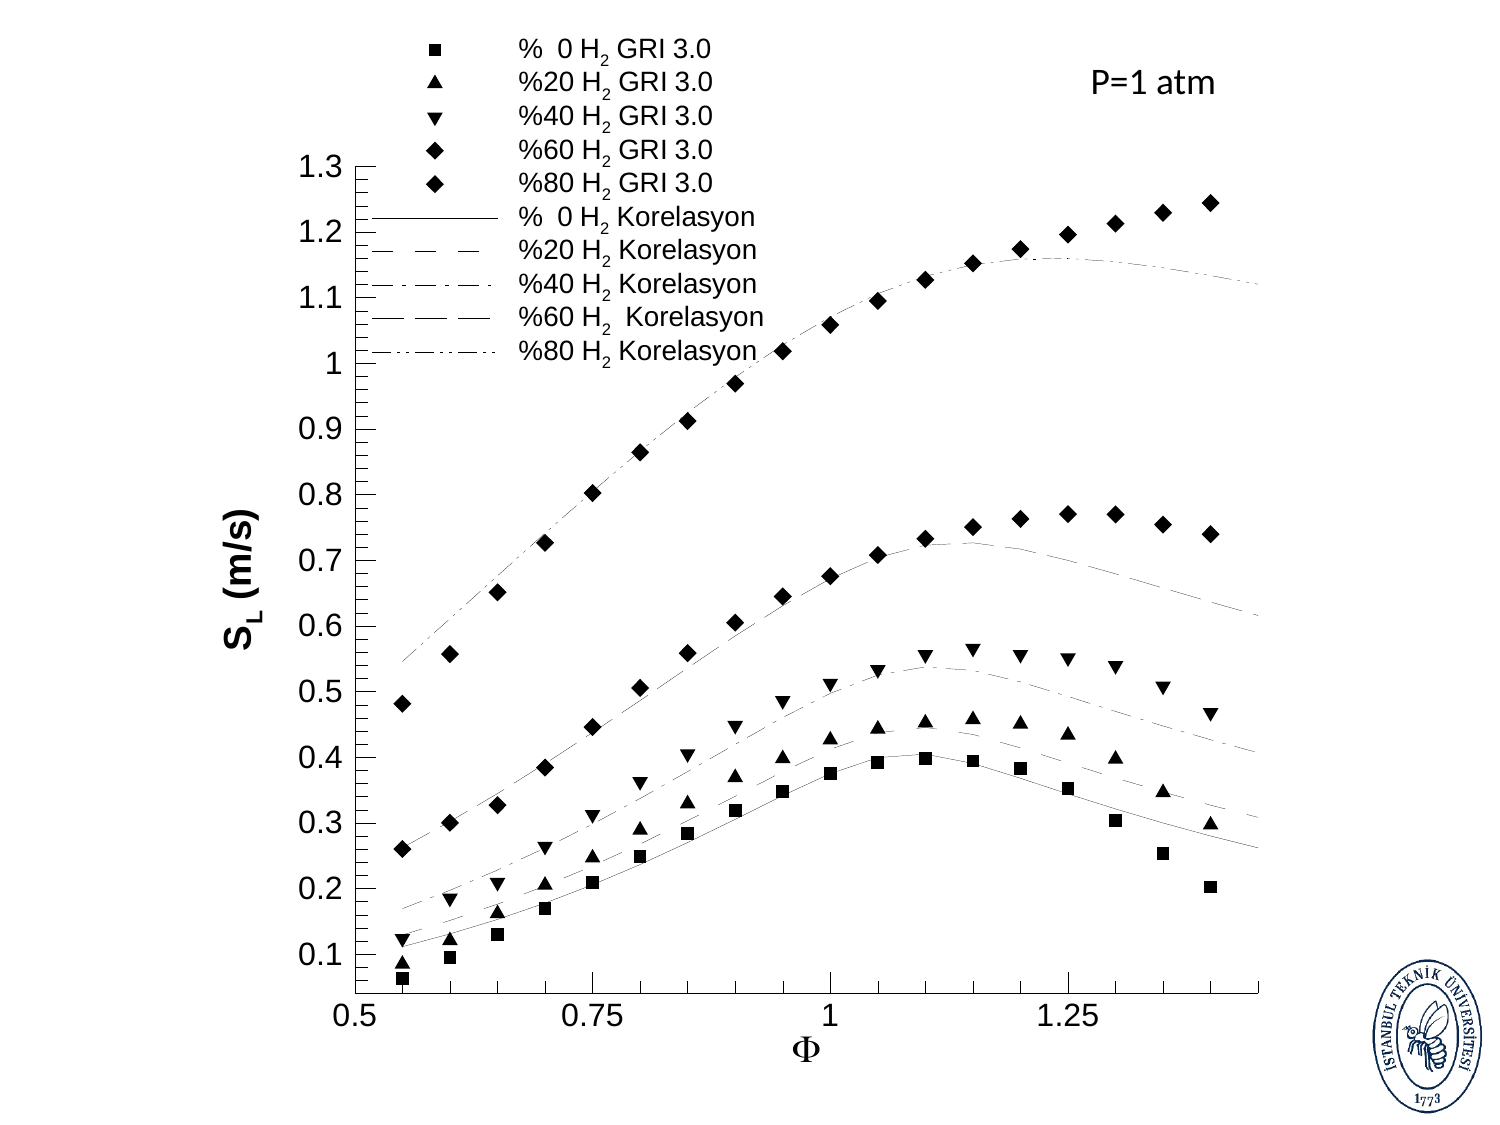
\includegraphics[width=0.85\linewidth,trim=10 40 10 40,clip]{slide81.png}
  \end{center}
\end{frame}

% =========================================================================
% Slide 82 -- SL vs phi P=3 atm
% =========================================================================
\begin{frame}{Laminar Flame Speed vs.\ $\phi$ ($P=3$ atm)}
  \begin{center}
    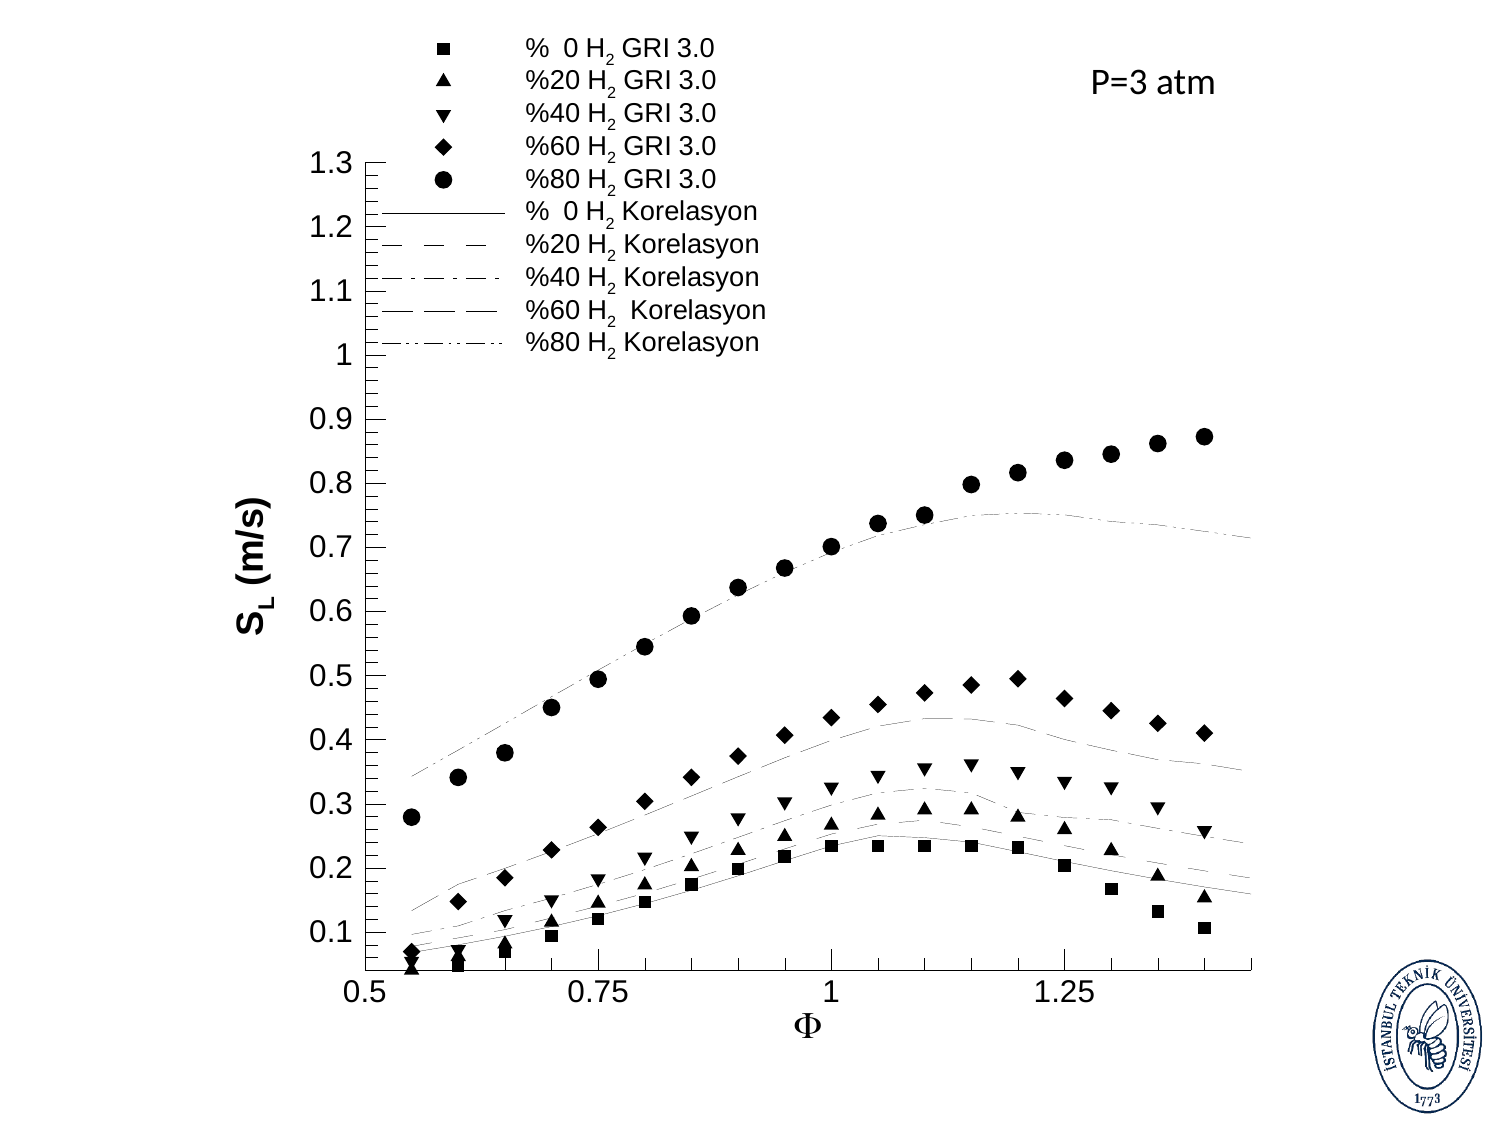
\includegraphics[width=0.85\linewidth,trim=10 40 10 40,clip]{slide82.png}
  \end{center}
\end{frame}

% =========================================================================
% Slide 83 -- NO vs phi P=1 atm
% =========================================================================
\begin{frame}{NO Emissions vs.\ $\phi$ ($P=1$ atm)}
  \begin{center}
    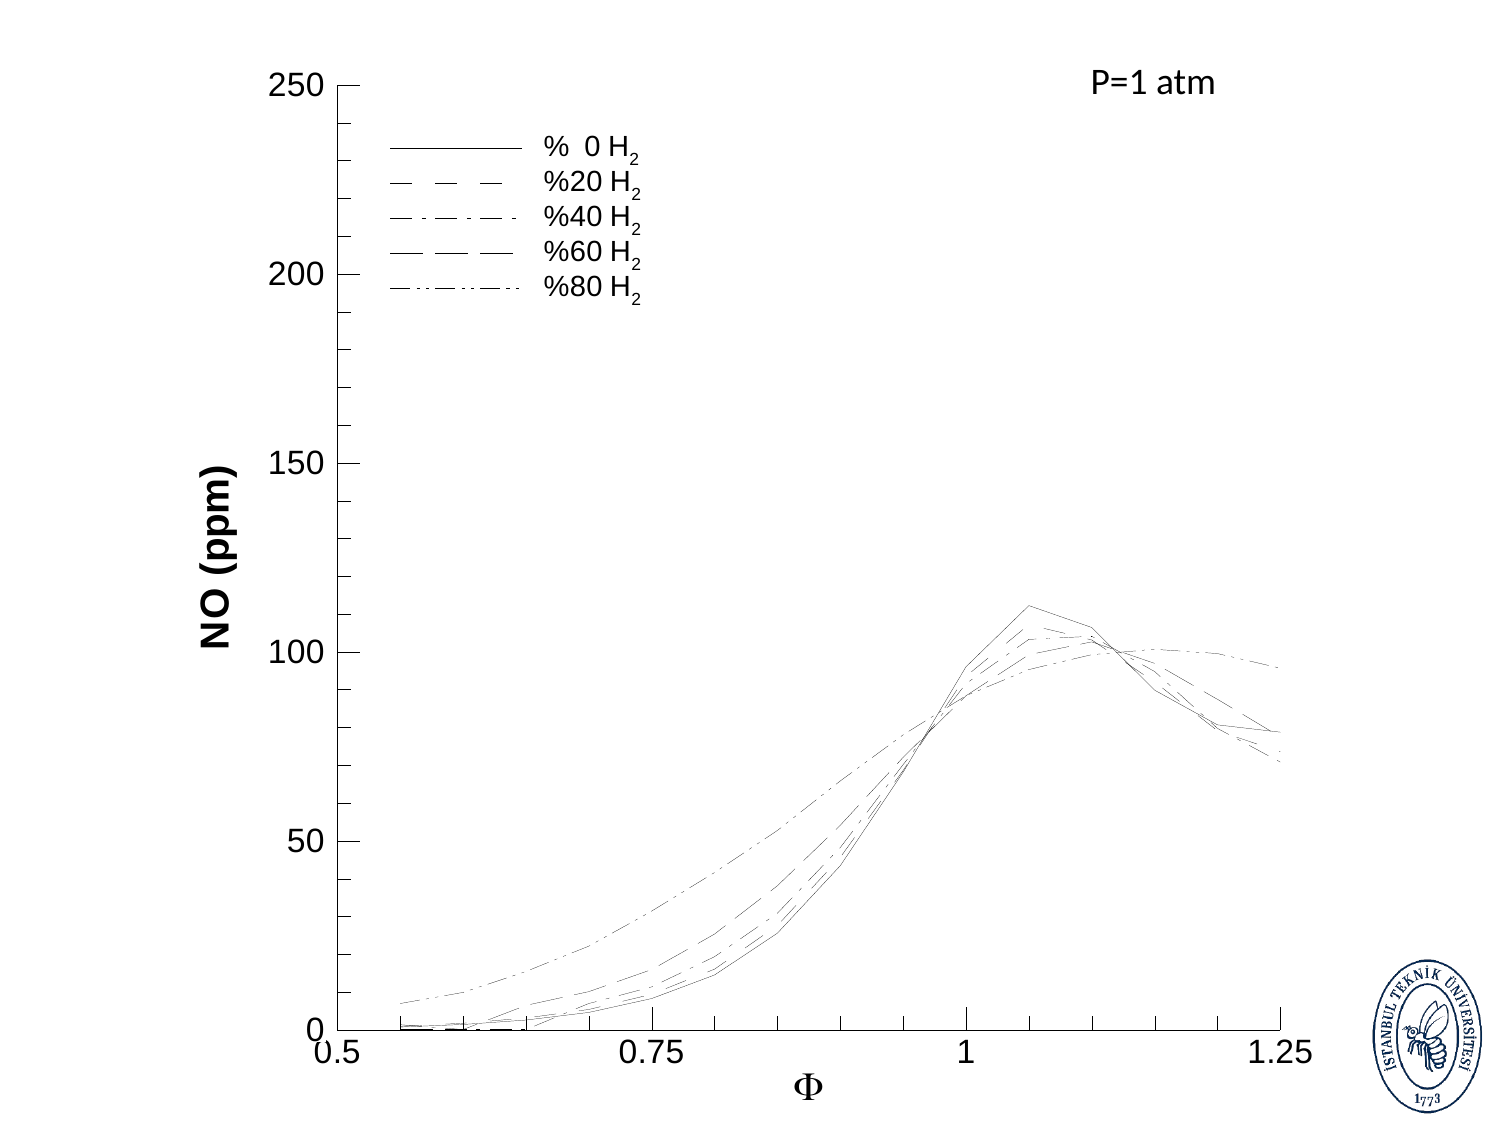
\includegraphics[width=0.85\linewidth,trim=10 40 10 40,clip]{slide83.png}
  \end{center}
\end{frame}

% =========================================================================
% Slide 84 -- NO vs phi P=3 atm
% =========================================================================
\begin{frame}{NO Emissions vs.\ $\phi$ ($P=3$ atm)}
  \begin{center}
    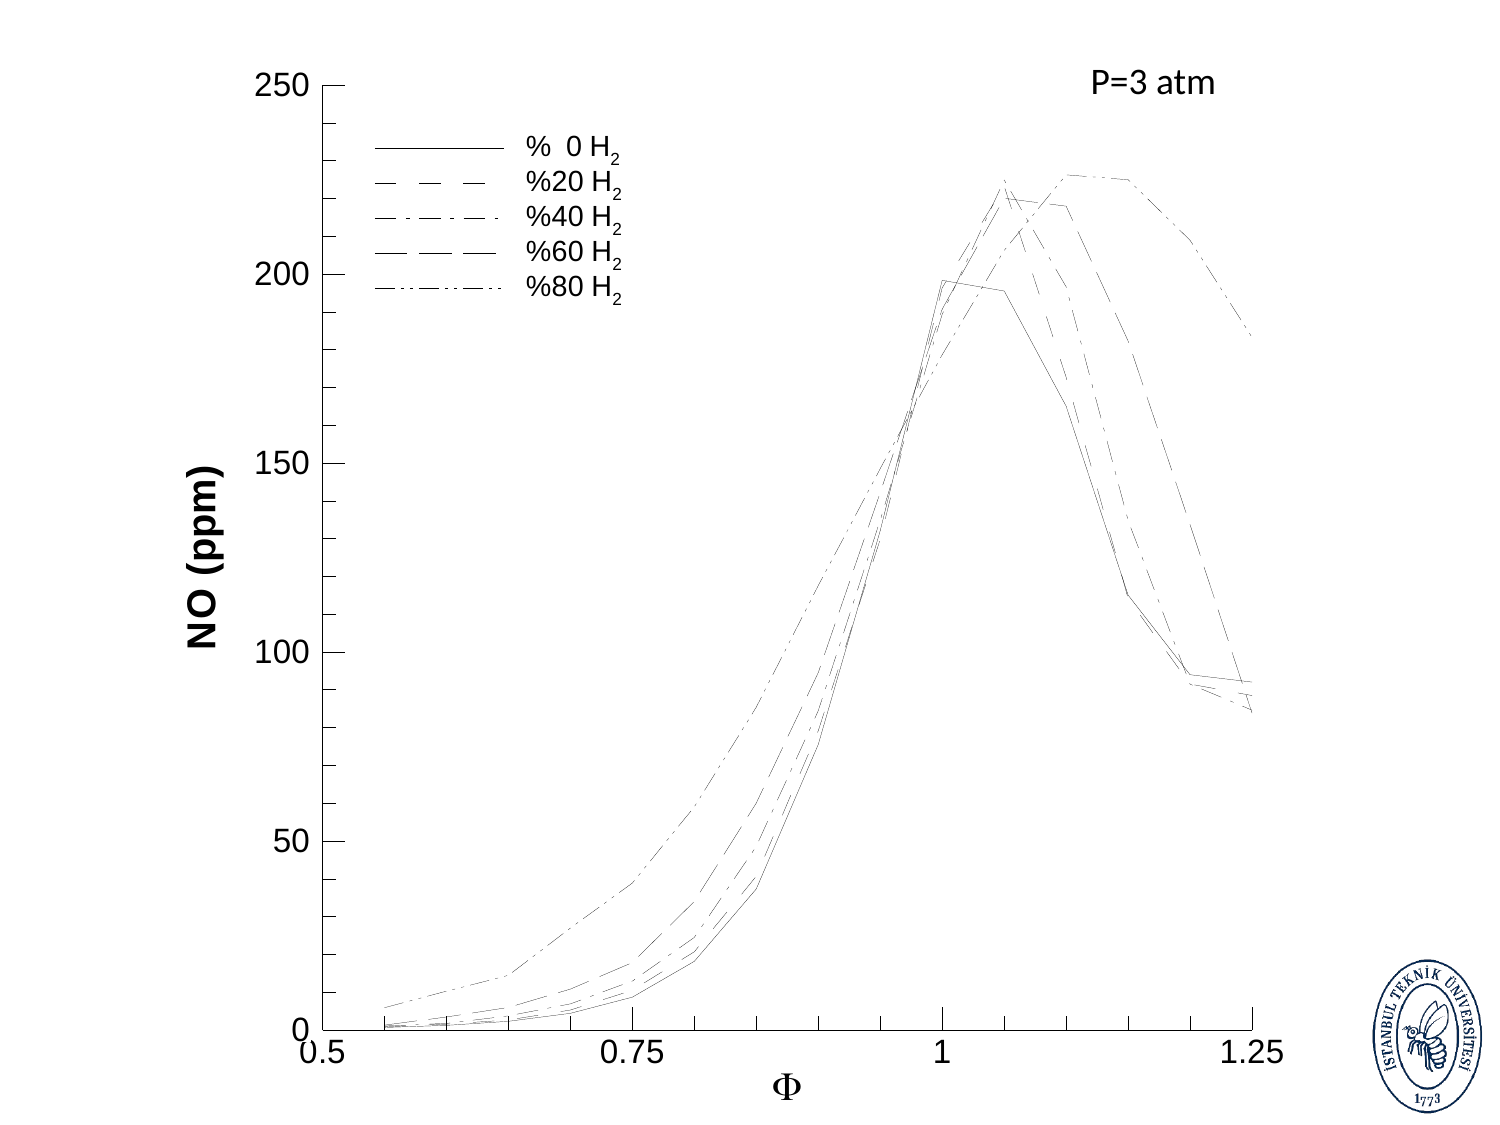
\includegraphics[width=0.85\linewidth,trim=10 40 10 40,clip]{slide84.png}
  \end{center}
\end{frame}

% =========================================================================
% Slide 85 -- NO/HO2 reaction path
% =========================================================================
\begin{frame}{Reaction Path Diagrams: NO and HO$_{2}$}
  \begin{center}
    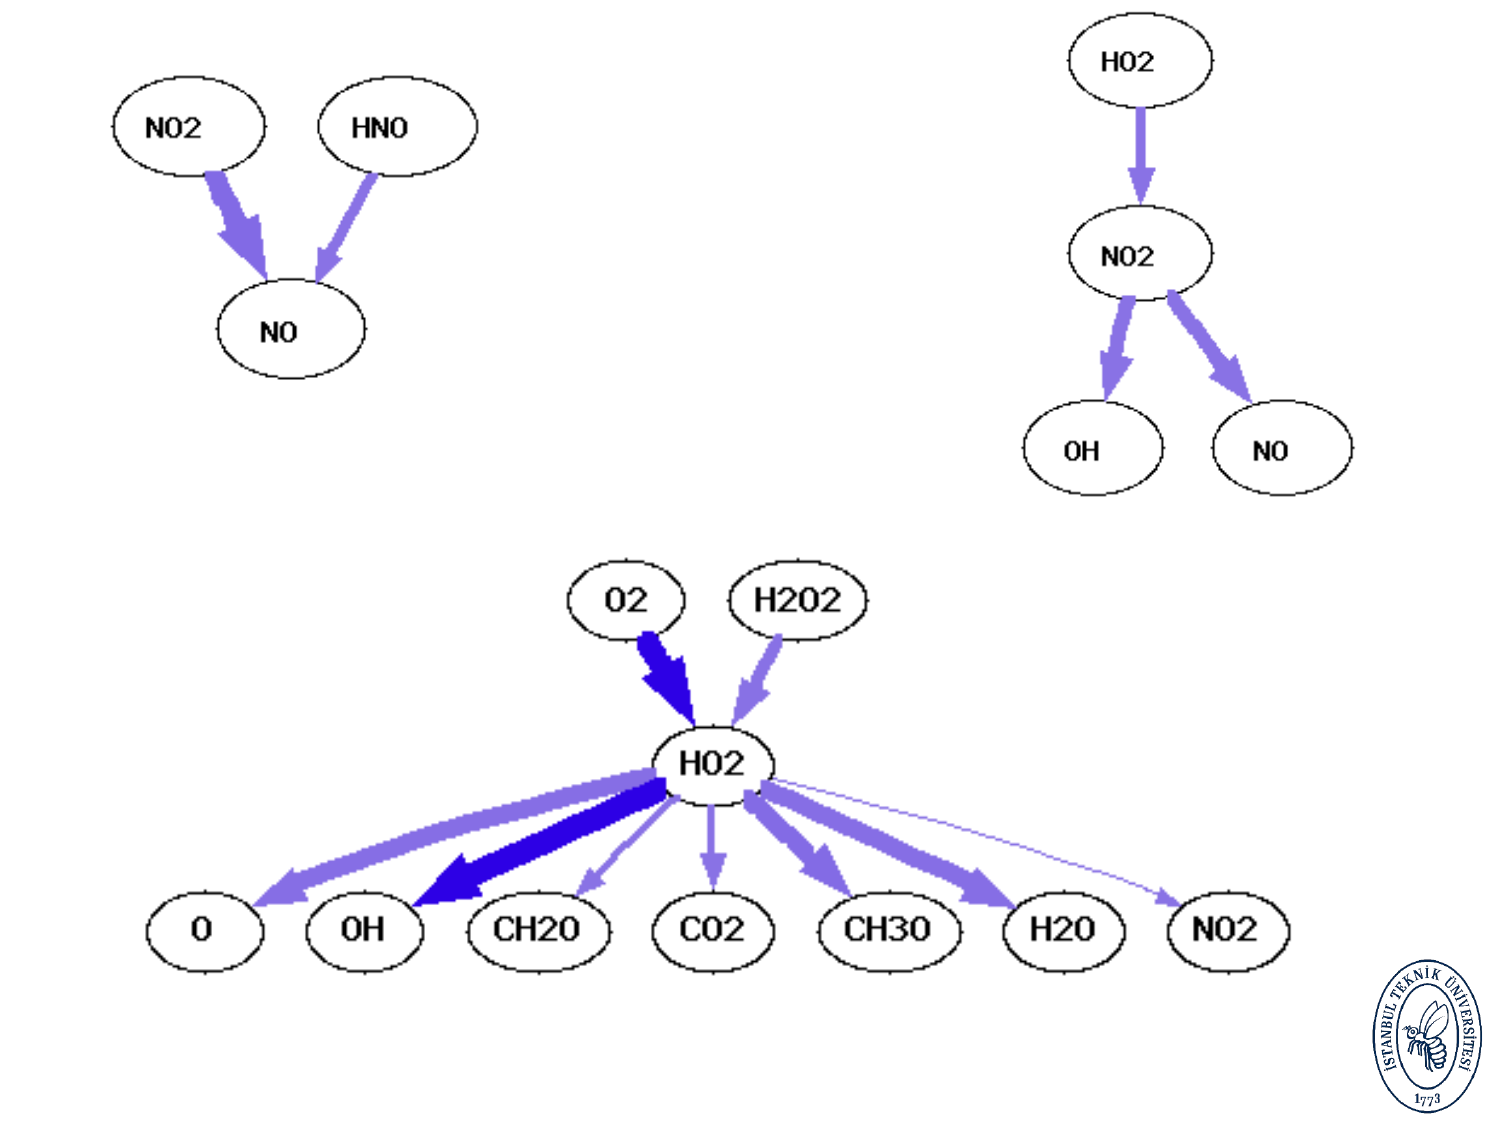
\includegraphics[width=0.85\linewidth,trim=10 40 10 40,clip]{slide85.png}
  \end{center}
\end{frame}

% =========================================================================
% Slide 86 -- Case Study II title
% =========================================================================
\begin{frame}[plain]
  \vfill
  \begin{center}
    {\Large\bfseries Case Study --- II}\\[8pt]
    {\large Cavity Flame Holding for High-Speed Reacting Flows}
  \end{center}
  \vfill
\end{frame}

% =========================================================================
% Slide 87 -- Ramjet schematic
% =========================================================================
\begin{frame}{Schematic of a Ramjet / Scramjet Engine}
  \begin{center}
    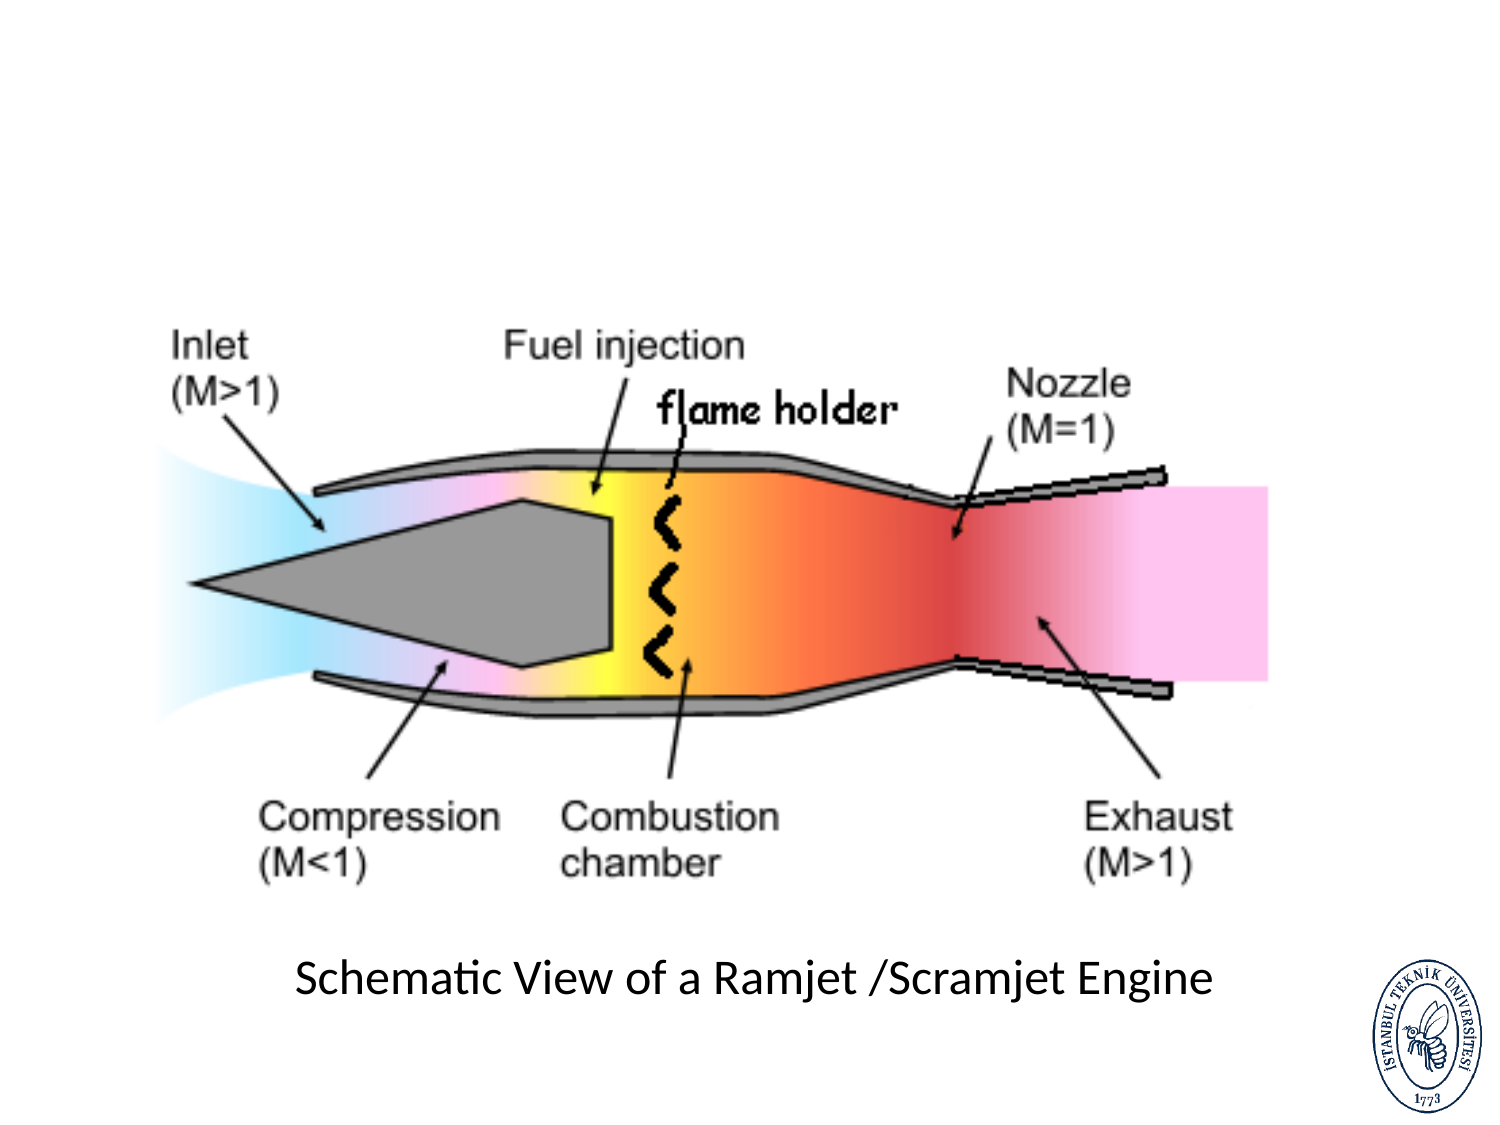
\includegraphics[width=0.85\linewidth,trim=10 40 10 40,clip]{slide87.png}
  \end{center}
\end{frame}

% =========================================================================
% Slide 88 -- Ramjet
% =========================================================================
\begin{frame}{Ramjet}
  \begin{columns}[t]
    \column{0.5\textwidth}
    \begin{itemize}
      \item Vehicle travels at supersonic speed
      \item Simplest air-breathing engine
      \item No moving parts
      \item Compression of intake achieved by supersonic flow --- inlet
            speed reduction (shock-wave system)
      \item Relatively low velocity
      \item Combustion at subsonic speeds
    \end{itemize}
    \column{0.5\textwidth}
    \begin{itemize}
      \item Very high reduction in speed
        \begin{itemize}
          \item High drag
          \item High fuel consumption
          \item Temperature at $\sim\!3000$~K
        \end{itemize}
      \item Diffuser
        \begin{itemize}
          \item Exit plane contracts
          \item Exhaust at supersonic speed
          \item Travel: $M = 3$
          \item Combustion: $M = 0.3$
        \end{itemize}
    \end{itemize}
  \end{columns}
\end{frame}

% =========================================================================
% Slide 89 -- Scramjet
% =========================================================================
\begin{frame}{Scramjet}
  \begin{itemize}
    \item Hypersonic flight
    \item No moving parts
    \item Combustion at supersonic speed
      \begin{itemize}
        \item Flow ignites supersonically
        \item Fuel injection into supersonic air stream
        \item Steer clear of shock waves
      \end{itemize}
    \item Aerodynamically challenged
  \end{itemize}
\end{frame}

% =========================================================================
% Slide 90 -- Specific impulse comparison
% =========================================================================
\begin{frame}{Comparison of Specific Impulses for Air-Breathing Engines}
  \begin{center}
    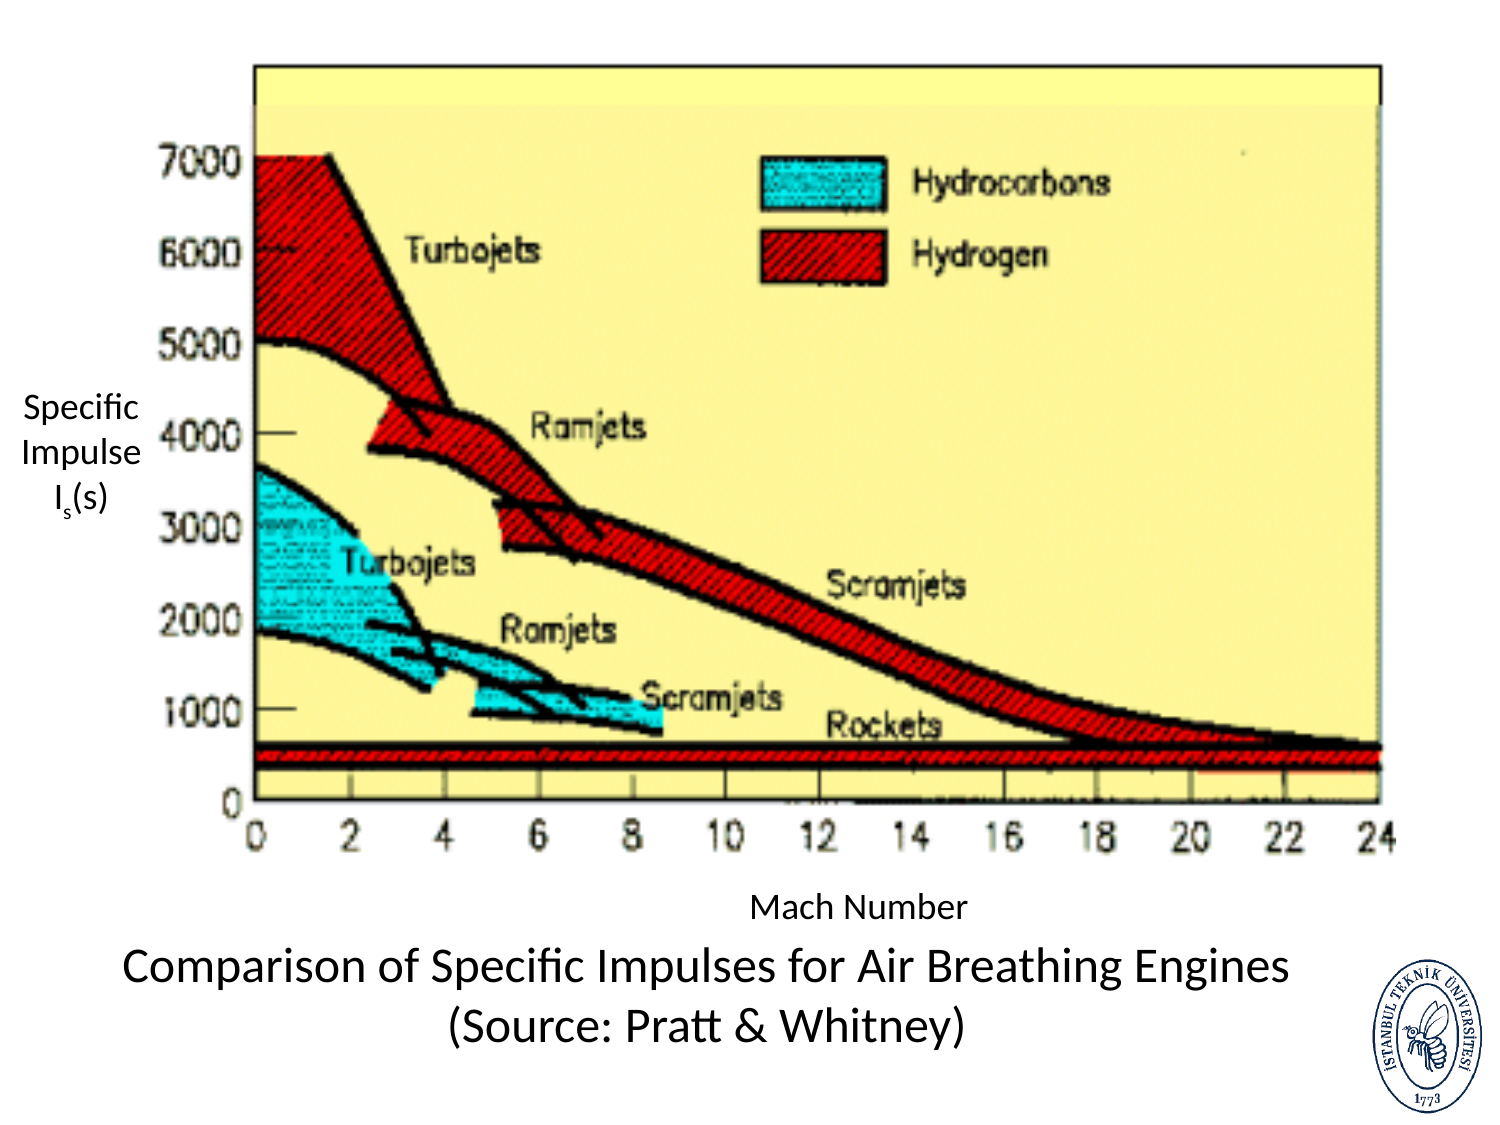
\includegraphics[width=0.8\linewidth,trim=10 40 10 40,clip]{slide90.png}
  \end{center}
  \begin{center}\footnotesize Source: Pratt \& Whitney\end{center}
\end{frame}

% =========================================================================
% Slide 91 -- Quote
% =========================================================================
\begin{frame}{}
  \vfill
  \begin{center}
    \begin{minipage}{0.85\linewidth}
      \itshape\large
      ``Sustaining supersonic combustion is like trying to light a match
      in a hurricane.''
      \par\vspace{6pt}
      \raggedleft\normalsize\upshape --- Richard J. Weber
    \end{minipage}
  \end{center}
  \vfill
\end{frame}

% =========================================================================
% Slide 92 -- Combustor schematic
% =========================================================================
\begin{frame}{Schematic of the Combustor}
  \begin{center}
    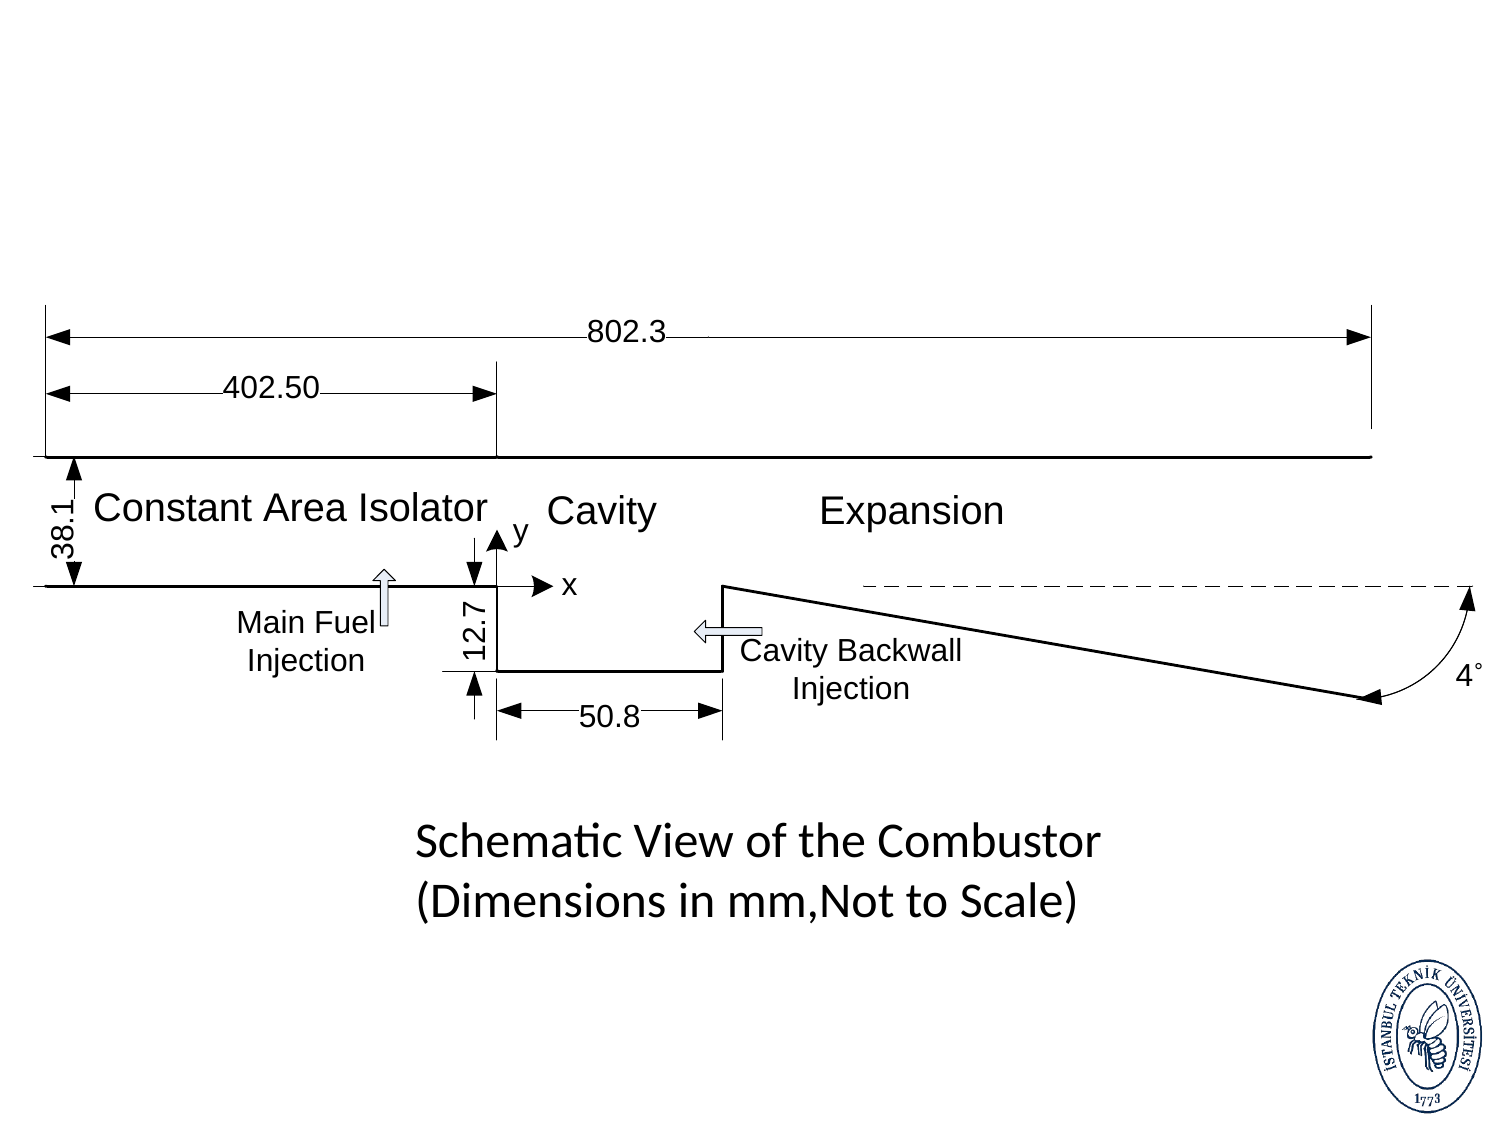
\includegraphics[width=0.85\linewidth,trim=10 40 10 40,clip]{slide92.png}
  \end{center}
  \begin{center}\footnotesize Dimensions in mm; not to scale.\end{center}
\end{frame}

% =========================================================================
% Slide 93 -- Conservation equations RANS (mass + momentum)
% =========================================================================
\begin{frame}{Conservation Equations}
  \begin{block}{Mass conservation}
    \[
      \pd{\bar{\rho}}{t} + \pd{}{x_{j}}\!\bigl(\bar{\rho}\tilde{u}_{j}\bigr) \;=\; 0
    \]
  \end{block}
  \begin{block}{Conservation of momentum}
    \[
      \pd{}{t}\!\bigl(\bar{\rho}\tilde{u}_{i}\bigr) + \pd{}{x_{j}}\!\bigl(\bar{\rho}\tilde{u}_{i}\tilde{u}_{j}\bigr)
        \;=\; -\pd{\bar{P}}{x_{i}}
              + \pd{}{x_{j}}\!\Bigl(\mu_{\mathrm{eff}}\!\Bigl(\pd{\tilde{u}_{i}}{x_{j}}+\pd{\tilde{u}_{j}}{x_{i}}\Bigr)
                            - \tfrac{2}{3}\mu_{\mathrm{eff}}\,\pd{\tilde{u}_{k}}{x_{k}}\,\delta_{ij}\Bigr)
    \]
  \end{block}
  \begin{block}{Effective viscosity}
    \[
      \mu_{\mathrm{eff}} \;=\; \mu + \mu_{t}
    \]
  \end{block}
\end{frame}

% =========================================================================
% Slide 94 -- Species/energy/state RANS
% =========================================================================
\begin{frame}{Conservation Equations (continued)}
  \begin{block}{Species conservation}
    \[
      \pd{}{t}\!\bigl(\bar{\rho}\tilde{Y}_{m}\bigr) + \pd{}{x_{j}}\!\bigl(\bar{\rho}\tilde{Y}_{m}\tilde{u}_{j}\bigr)
        \;=\; R_{k,m} - \pd{}{x_{j}}\!\Bigl(\tilde{J}_{j} + \frac{\mu_{t}}{\mathrm{Sc}_{t}}\,\pd{\tilde{Y}_{m}}{x_{j}}\Bigr)
    \]
    \[
      \tilde{J}_{j} \;=\; -\bar{\rho}\mathcal{D}\,\pd{\tilde{Y}_{m}}{x_{j}}
    \]
  \end{block}
  \begin{block}{Conservation of energy}
    \[
      \pd{}{t}\!\bigl(\bar{\rho}\tilde{H}\bigr) + \pd{}{x_{j}}\!\bigl(\bar{\rho}\tilde{H}\tilde{u}_{j}\bigr)
        \;=\; \pd{\bar{P}}{t} + \pd{}{x_{j}}\!\Bigl(\lambda\,\pd{\tilde{T}}{x_{j}}+\frac{\mu_{t}}{\mathrm{Pr}_{t}}\pd{\tilde{H}}{x_{j}}\Bigr)
    \]
  \end{block}
  \begin{block}{Equation of state}
    \[
      \bar{P} \;=\; \bar{\rho}\,R\,(\tilde{Y}_{m})\,\tilde{T}
    \]
  \end{block}
\end{frame}

% =========================================================================
% Slide 95 -- Turbulence modelling
% =========================================================================
\begin{frame}{Turbulence Modelling (SST $k$--$\omega$)}
  \scriptsize
  \begin{block}{Kinetic energy transport}
    \[
      \pd{(\bar{\rho} k)}{t} + \pd{(\bar{\rho}\tilde{u}_{j} k)}{x_{j}}
        \;=\; P_{k} - \beta^{*}\bar{\rho}k\omega
              + \pd{}{x_{j}}\!\Bigl[\!\Bigl(\mu+\frac{\mu_{t}}{\sigma_{k3}}\Bigr)\pd{k}{x_{j}}\Bigr]
    \]
  \end{block}
  \begin{block}{Inverse time-scale transport}
    \[
      \pd{(\bar{\rho}\omega)}{t} + \pd{(\bar{\rho}\tilde{u}_{j}\omega)}{x_{j}}
        = \alpha_{3}\frac{\omega}{k}P_{k} - \beta_{3}\bar{\rho}\omega^{2}
              + \pd{}{x_{j}}\!\Bigl[\!\Bigl(\mu+\frac{\mu_{t}}{\sigma_{\omega3}}\Bigr)\pd{\omega}{x_{j}}\Bigr]
              + (1-F_{1})\,2\bar{\rho}\sigma_{\omega2}\frac{1}{\omega}\pd{k}{x_{j}}\pd{\omega}{x_{j}}
    \]
  \end{block}
  \begin{block}{Turbulent kinetic energy production}
    \[
      P_{k} \;=\; \mu_{t}\!\Bigl(\pd{\tilde{u}_{i}}{x_{j}}+\pd{\tilde{u}_{j}}{x_{i}}\Bigr)\pd{\tilde{u}_{i}}{x_{j}}
              - \tfrac{2}{3}\delta_{ij}\!\Bigl(\bar{\rho}k+\mu_{t}\pd{\tilde{u}_{k}}{x_{k}}\Bigr)\pd{\tilde{u}_{i}}{x_{j}}
    \]
    \[
      \Phi_{3} \;=\; F_{1}\Phi_{1} + (1-F_{1})\Phi_{2}
    \]
  \end{block}
\end{frame}

% =========================================================================
% Slide 96 -- Modelling parameters
% =========================================================================
\begin{frame}{SST $k$--$\omega$ Modelling Parameters}
  \scriptsize
  \begin{columns}[T]
    \column{0.58\textwidth}
    \[
      a_{1} = 0.31, \qquad
      \nu_{t} = \frac{a_{1}k}{\max(a_{1}\omega,\,SF_{2})}
    \]
    \[
      \mu_{t} = \bar{\rho}\,\nu_{t}
    \]
    Invariant measure of strain rate:
    \[
      S \;=\; \sqrt{\!\Bigl(\pd{\tilde{u}_{i}}{x_{j}}+\pd{\tilde{u}_{j}}{x_{i}}\Bigr)\pd{\tilde{u}_{i}}{x_{j}}}
    \]
    Blending functions:
    \[
      F_{1} = \tanh\!\bigl(\arg_{1}^{4}\bigr), \quad
      F_{2} = \tanh\!\bigl(\arg_{2}^{2}\bigr)
    \]
    \[
      \arg_{1} = \min\!\!\left[\max\!\!\left(\!\tfrac{\sqrt{k}}{\beta^{*}\omega y},\tfrac{500\nu}{y^{2}\omega}\right)\!,\tfrac{4\bar{\rho}\sigma_{\omega2}k}{CD_{k\omega}y^{2}}\right]
    \]
    \[
      \arg_{2} = \max\!\!\left(\!2\tfrac{\sqrt{k}}{\beta^{*}\omega y},\,\tfrac{500\nu}{y^{2}\omega}\right)
    \]
    \column{0.42\textwidth}
    \begin{block}{Constants}
      \begin{tabular}{ll}
        $\alpha_{1}$       & $5/9$ \\
        $\alpha_{2}$       & $0.44$ \\
        $\beta_{1}$        & $3/40$ \\
        $\beta_{2}$        & $0.0828$ \\
        $\beta^{*}$        & $0.09$ \\
        $\sigma_{k1}$      & $2$ \\
        $\sigma_{k2}$      & $2$ \\
        $\sigma_{\omega1}$ & $2$ \\
        $\sigma_{\omega2}$ & $0.856$
      \end{tabular}
    \end{block}
  \end{columns}
\end{frame}

% =========================================================================
% Slide 97 -- Cavity reaction table
% =========================================================================
\begin{frame}{Reduced Hydrogen Combustion Mechanism}
  \begin{center}
    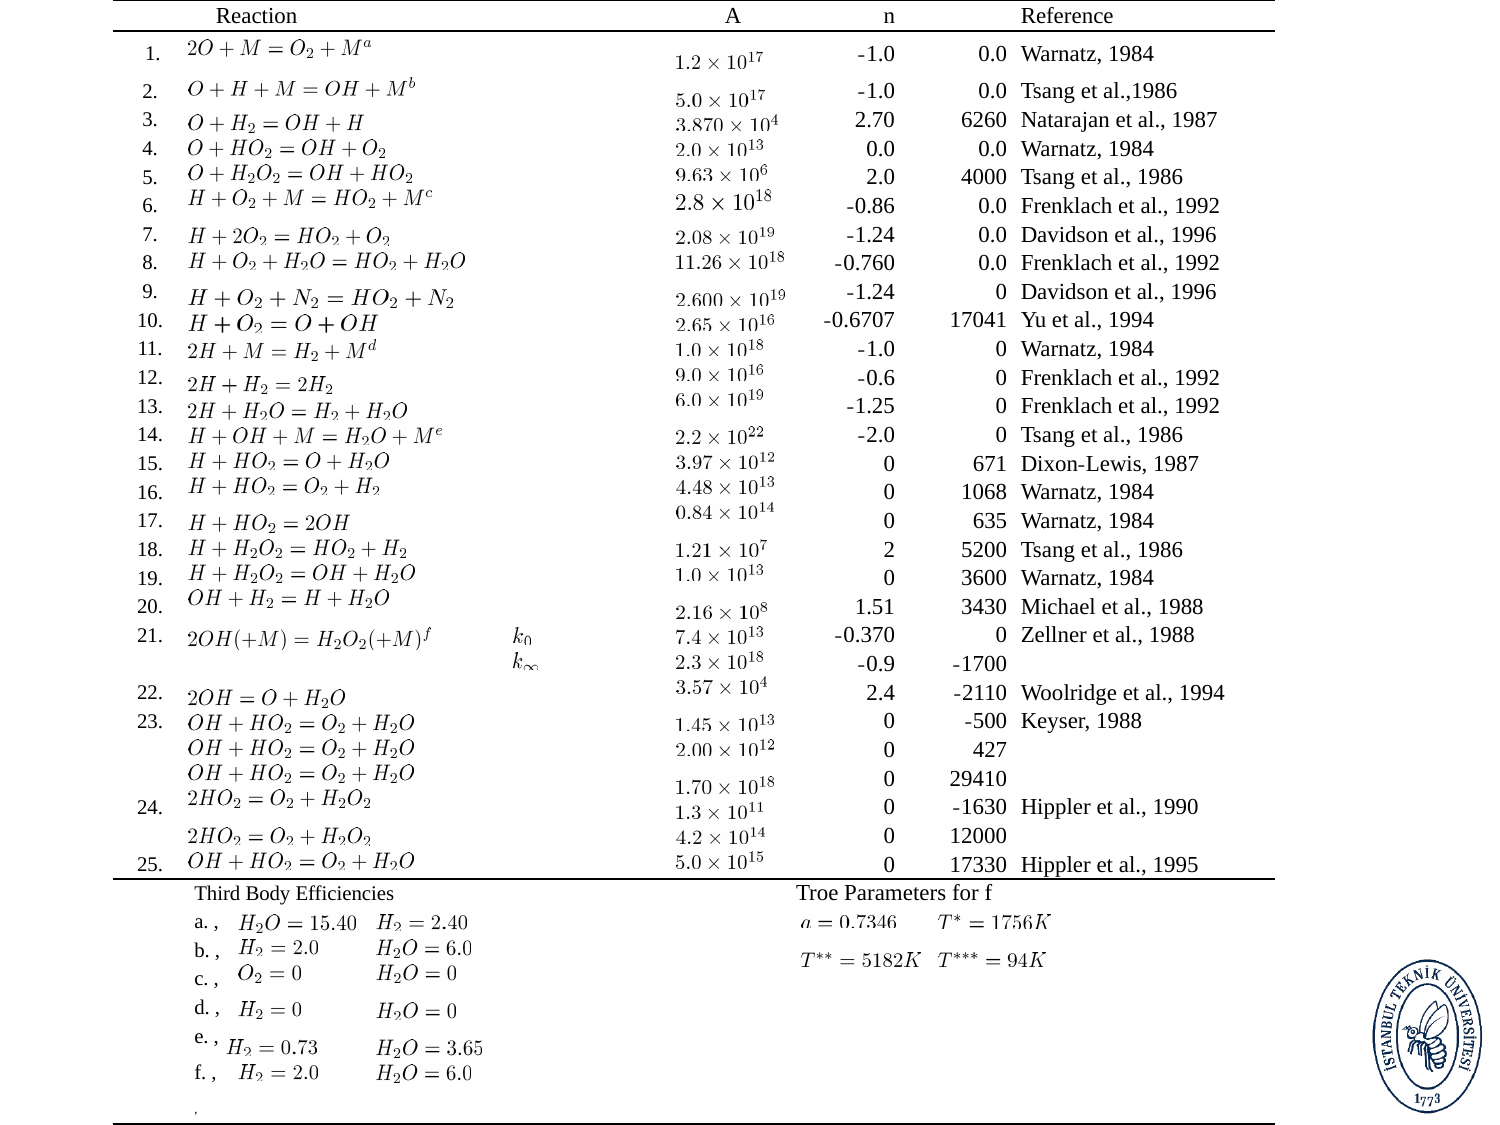
\includegraphics[width=0.95\linewidth,trim=10 40 10 40,clip]{slide97.png}
  \end{center}
\end{frame}

% =========================================================================
% Slide 98 -- Flame speed comparison
% =========================================================================
\begin{frame}{Validation: Flame Speed (Model vs.\ Experiment)}
  \begin{center}
    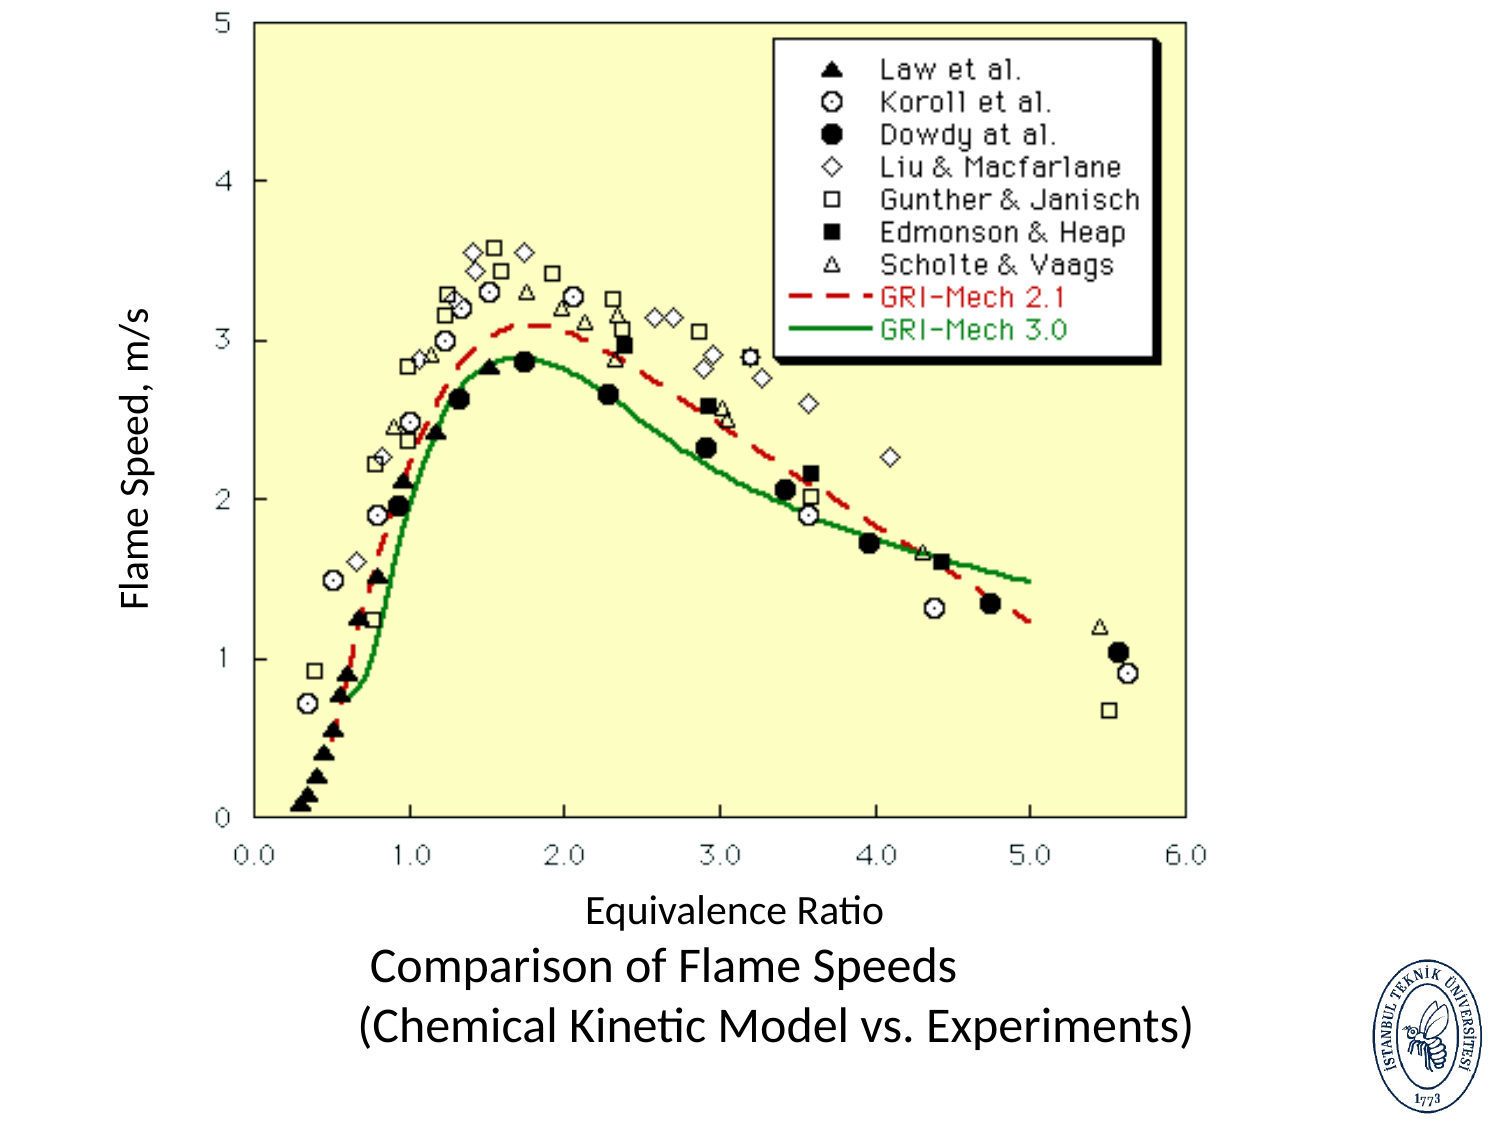
\includegraphics[width=0.85\linewidth,trim=10 40 10 40,clip]{slide98.png}
  \end{center}
\end{frame}

% =========================================================================
% Slide 99 -- Ignition delay comparison
% =========================================================================
\begin{frame}{Validation: Ignition Delay (Model vs.\ Experiment)}
  \begin{center}
    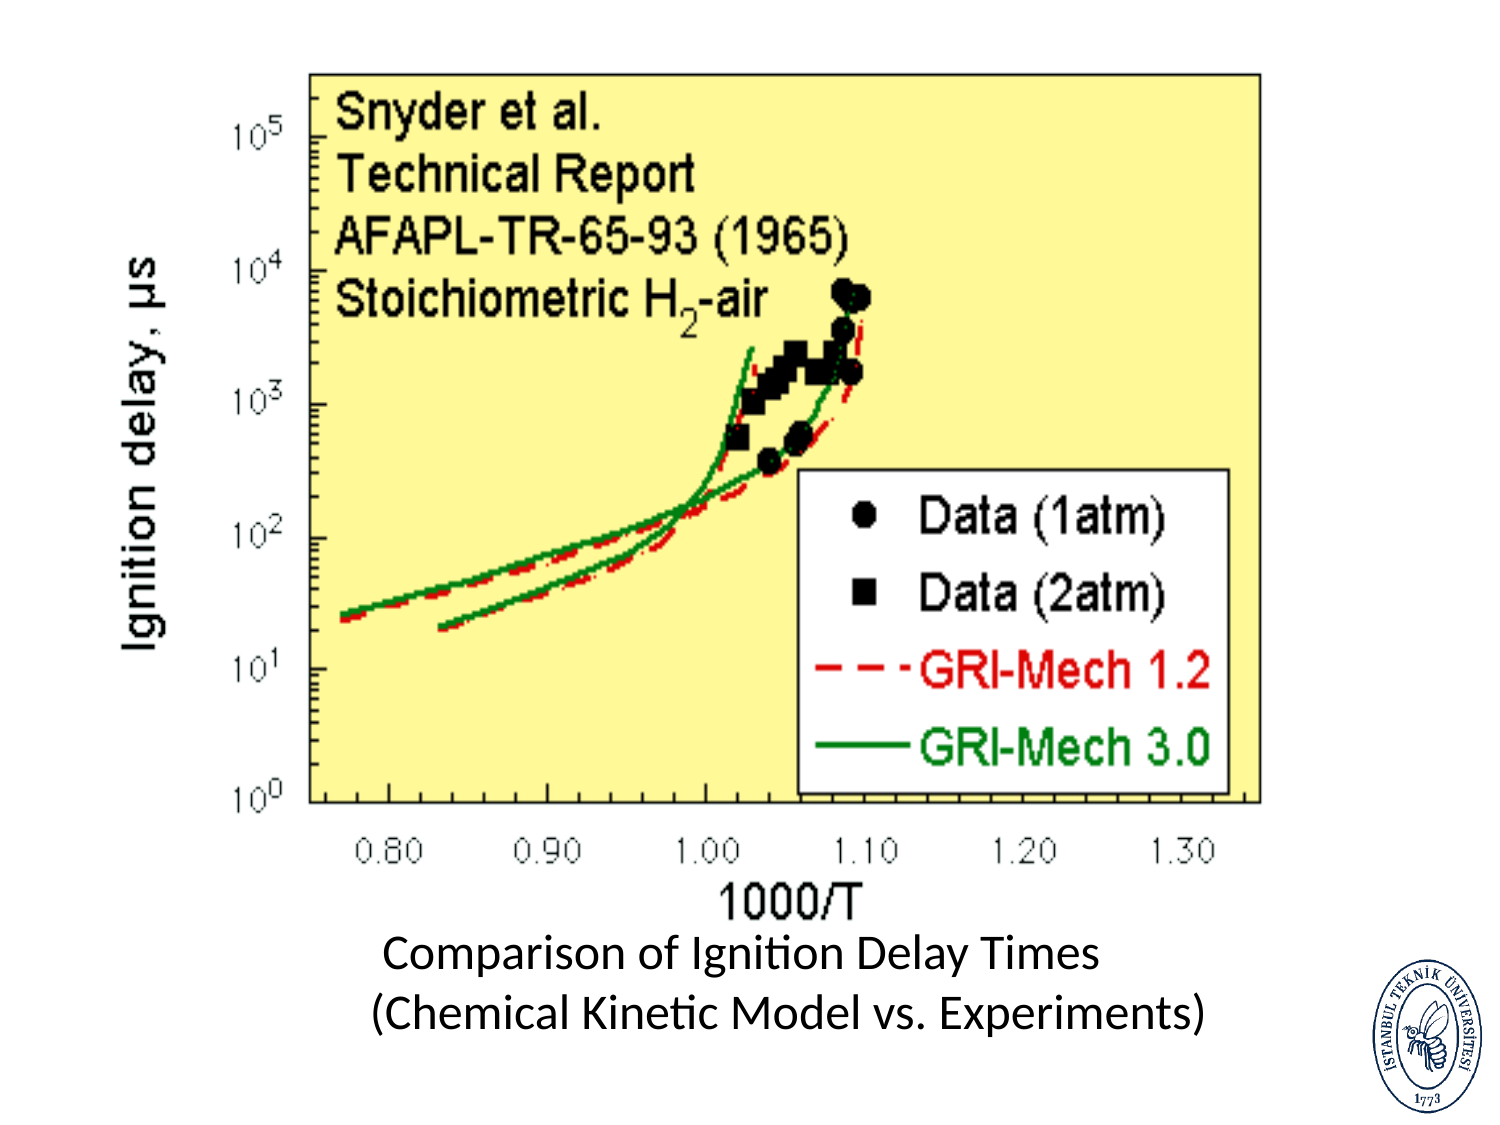
\includegraphics[width=0.85\linewidth,trim=10 40 10 40,clip]{slide99.png}
  \end{center}
\end{frame}

% =========================================================================
% Slide 100 -- Grid
% =========================================================================
\begin{frame}{Grid Structure in the Vicinity of the Cavity}
  \begin{center}
    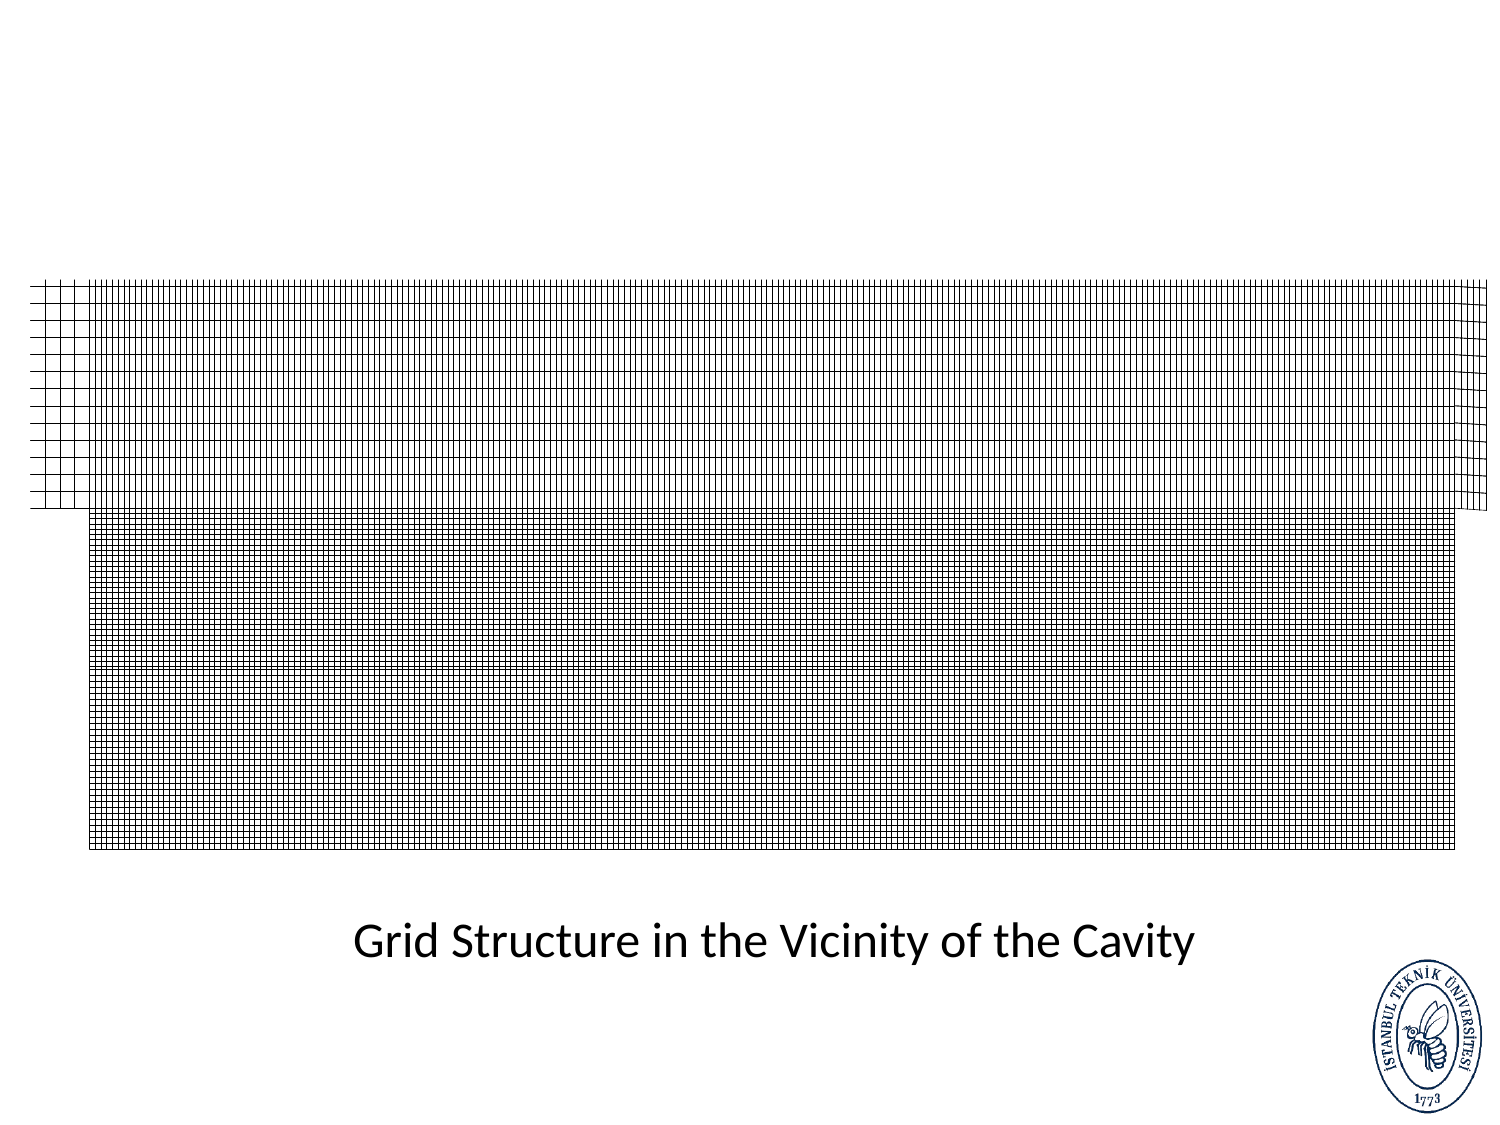
\includegraphics[width=0.85\linewidth,trim=10 40 10 40,clip]{slide100.png}
  \end{center}
\end{frame}

% =========================================================================
% Slide 101 -- Solver structure
% =========================================================================
\begin{frame}{Structure of the Solver}
  \begin{center}
    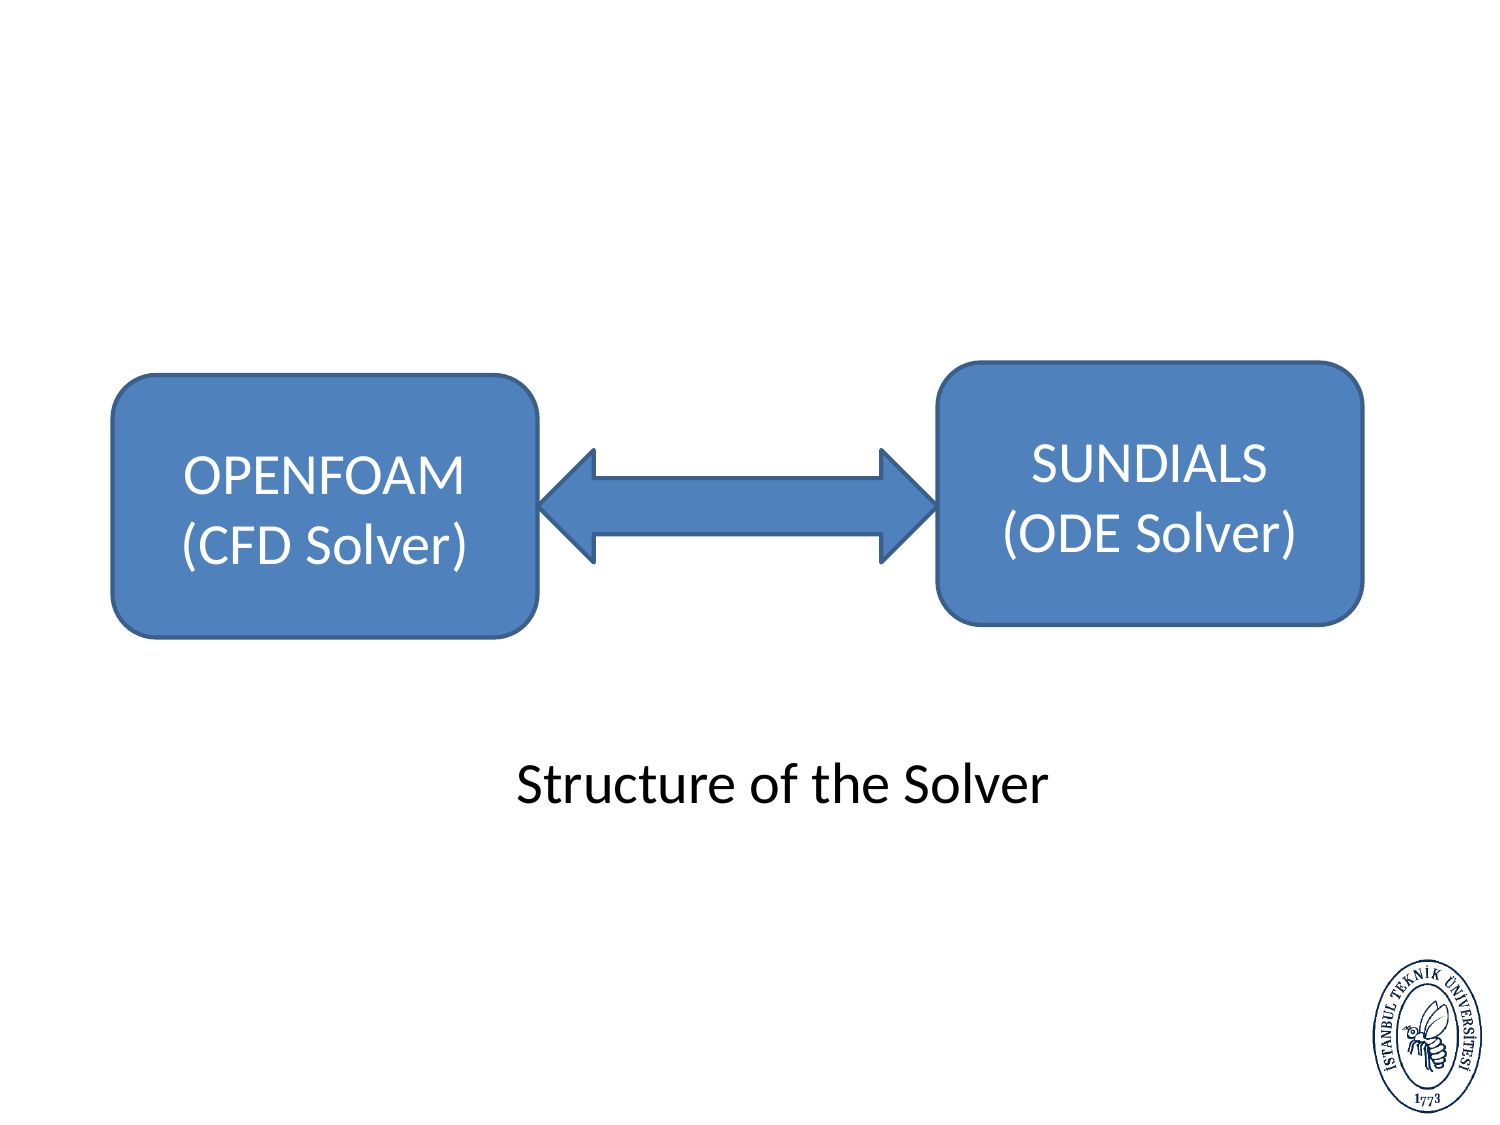
\includegraphics[width=0.65\linewidth,trim=10 40 10 40,clip]{slide101.png}
  \end{center}
  \begin{center}
    OpenFOAM (CFD solver) $\;\longleftrightarrow\;$ SUNDIALS (ODE solver)
  \end{center}
\end{frame}

% =========================================================================
% Slide 102 -- Flow parameters table
% =========================================================================
\begin{frame}{Flow Parameters for Air and Hydrogen}
  \begin{center}
  \begin{tabular}{lccc}
    \toprule
                                & Air  & H$_{2}$ (Upstream) & H$_{2}$ (Cavity) \\ \midrule
    $\dot{m}$ [kg/s]            & 3.4  & 0.002              & 0.001 \\
    $T_{0}$ [K]                 & 702  & 300                & 300   \\
    $M$                         & 1.4  & 1.0                & 0.5   \\
    $P$ [MPa]                   & 0.8  & 3.9                & 3.9   \\
    \bottomrule
  \end{tabular}
  \end{center}
\end{frame}

% =========================================================================
% Slide 103 -- Pressure distribution
% =========================================================================
\begin{frame}{Pressure Distribution within the Combustor}
  \begin{center}
    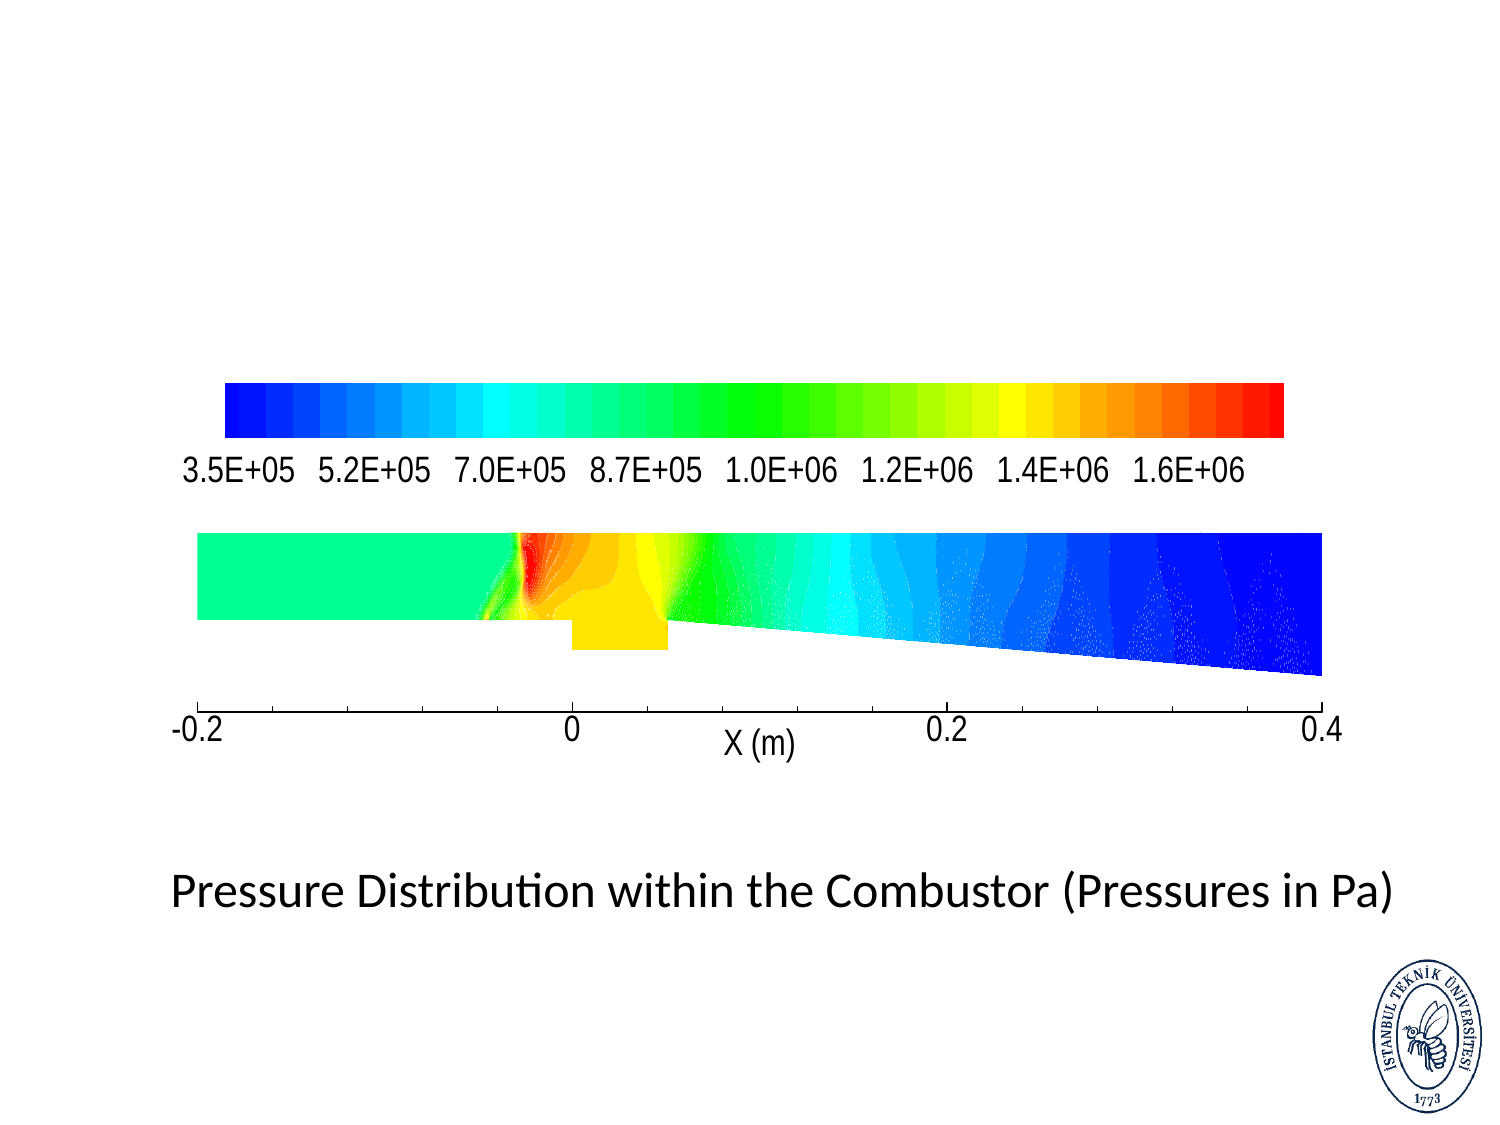
\includegraphics[width=0.95\linewidth,trim=10 40 10 40,clip]{slide103.png}
  \end{center}
  \begin{center}\footnotesize Pressures in Pa.\end{center}
\end{frame}

% =========================================================================
% Slide 104 -- Top wall pressure
% =========================================================================
\begin{frame}{Pressure Distribution Along the Top Surface}
  \begin{center}
    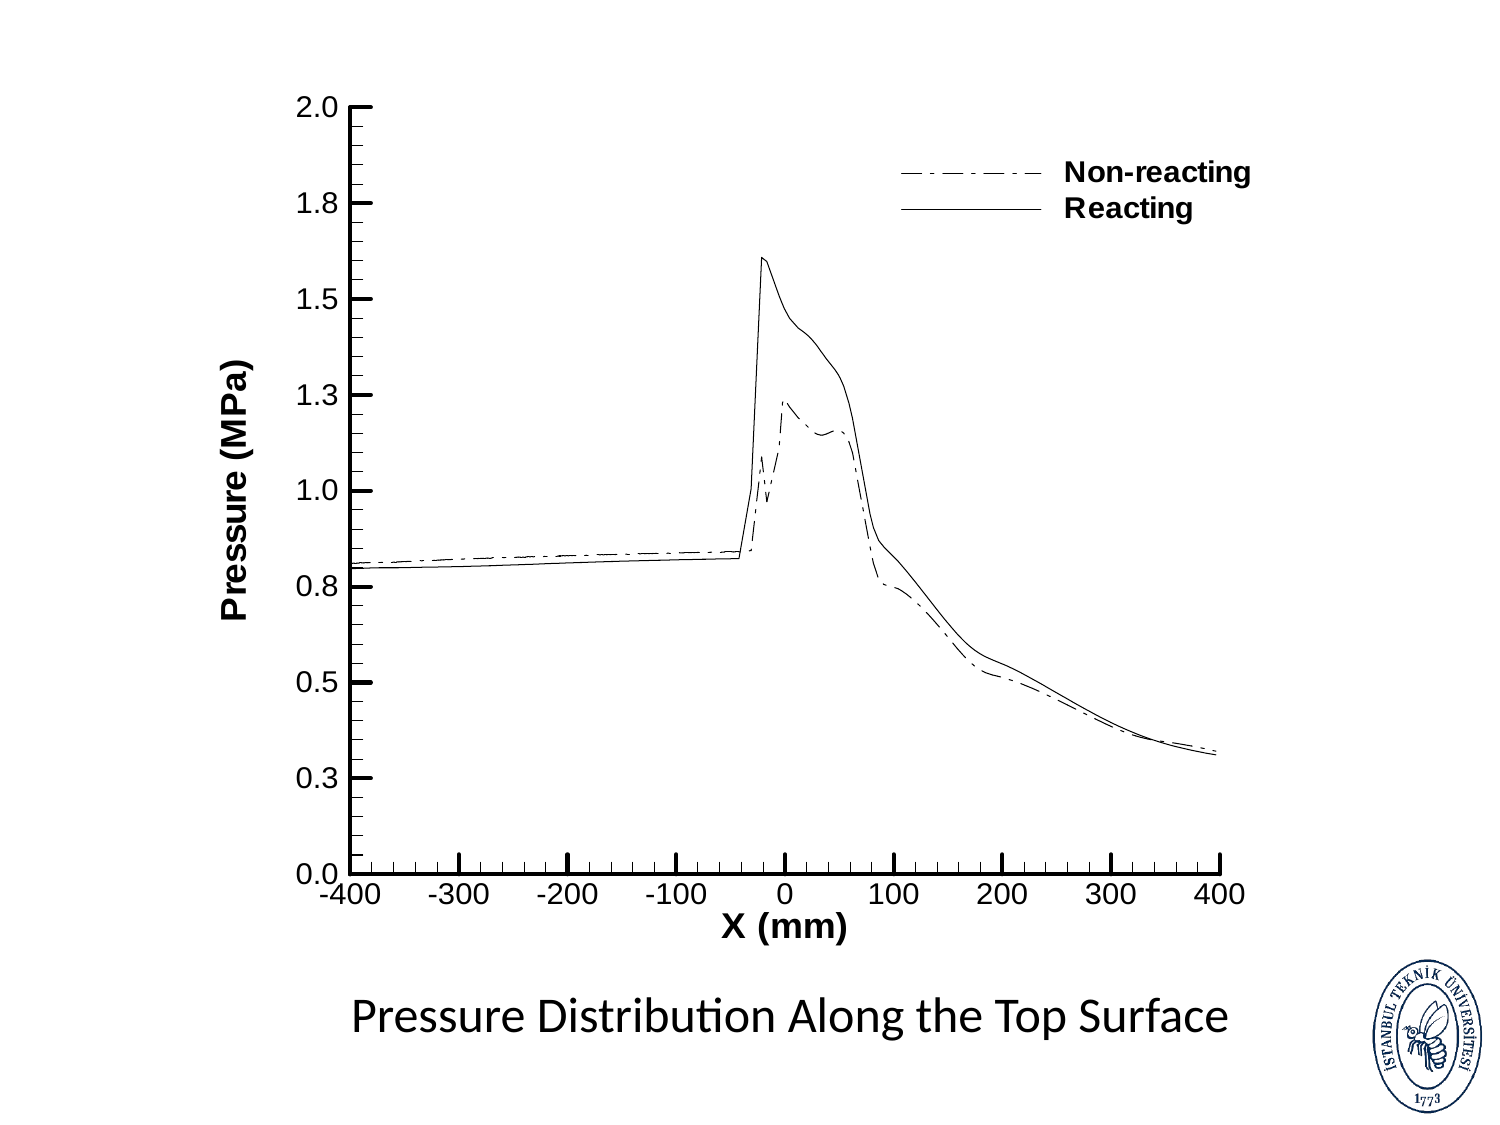
\includegraphics[width=0.85\linewidth,trim=10 40 10 40,clip]{slide104.png}
  \end{center}
\end{frame}

% =========================================================================
% Slide 105 -- Mach distribution
% =========================================================================
\begin{frame}{Mach Number Distribution within the Combustor}
  \begin{center}
    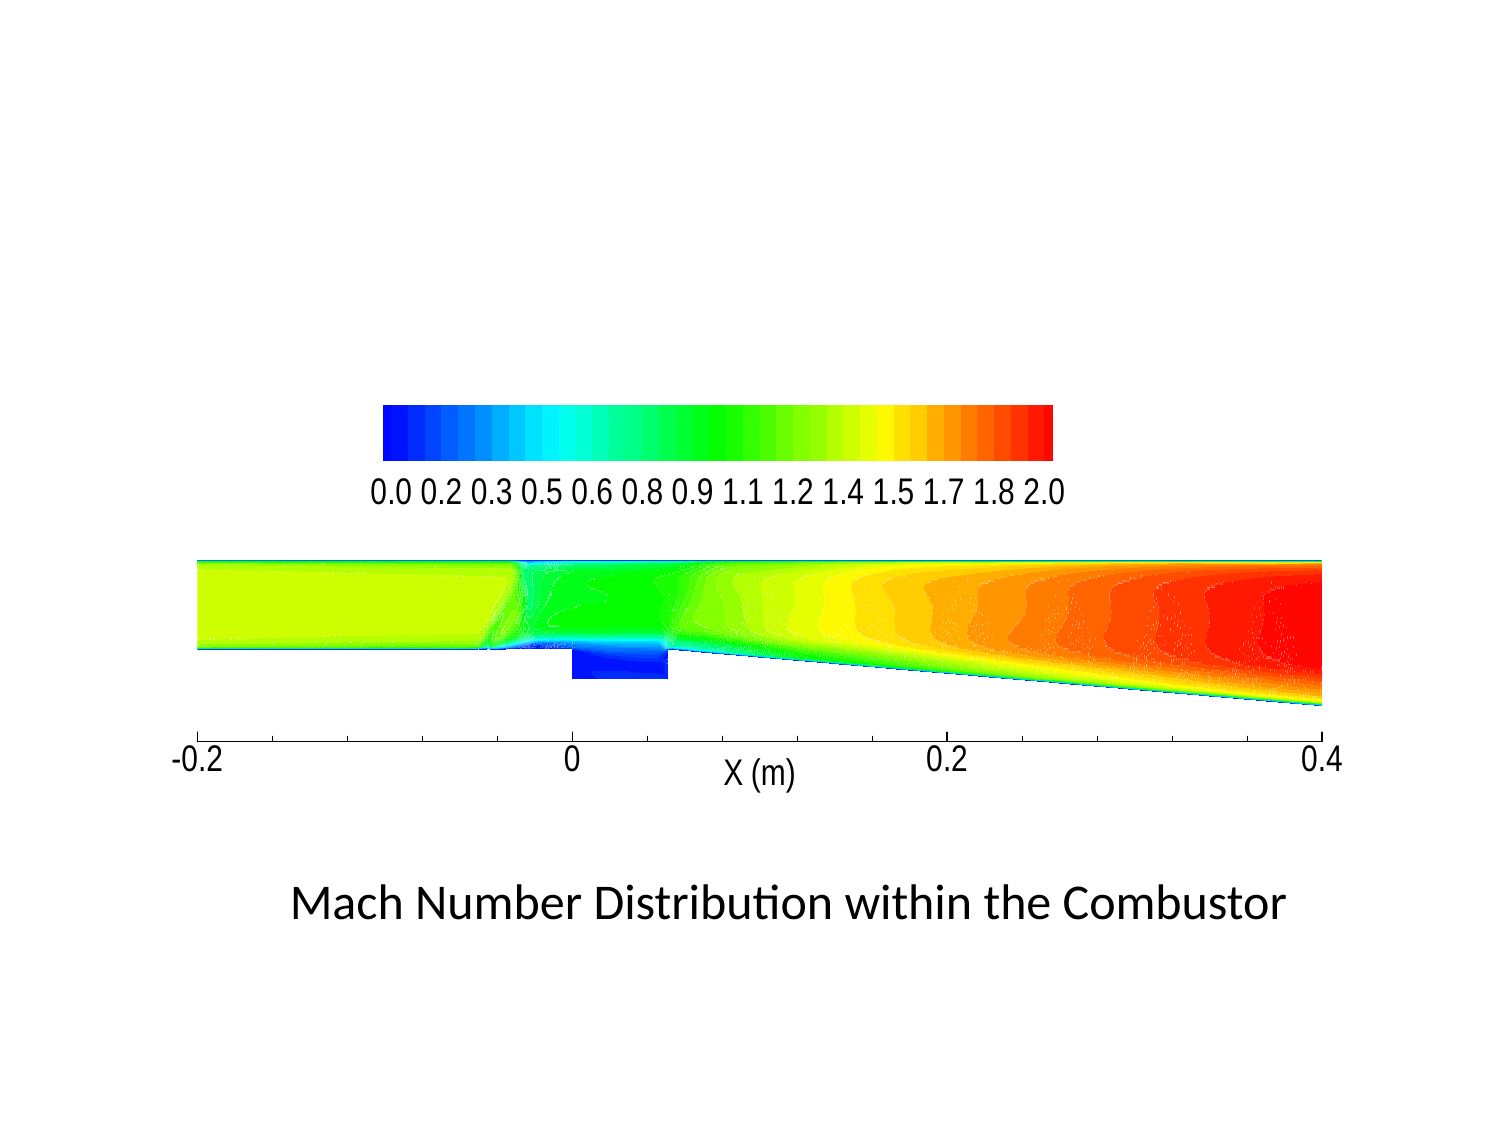
\includegraphics[width=0.95\linewidth,trim=10 40 10 40,clip]{slide105.png}
  \end{center}
\end{frame}

% =========================================================================
% Slide 106 -- Temperature distribution
% =========================================================================
\begin{frame}{Temperature Distribution within the Combustor}
  \begin{center}
    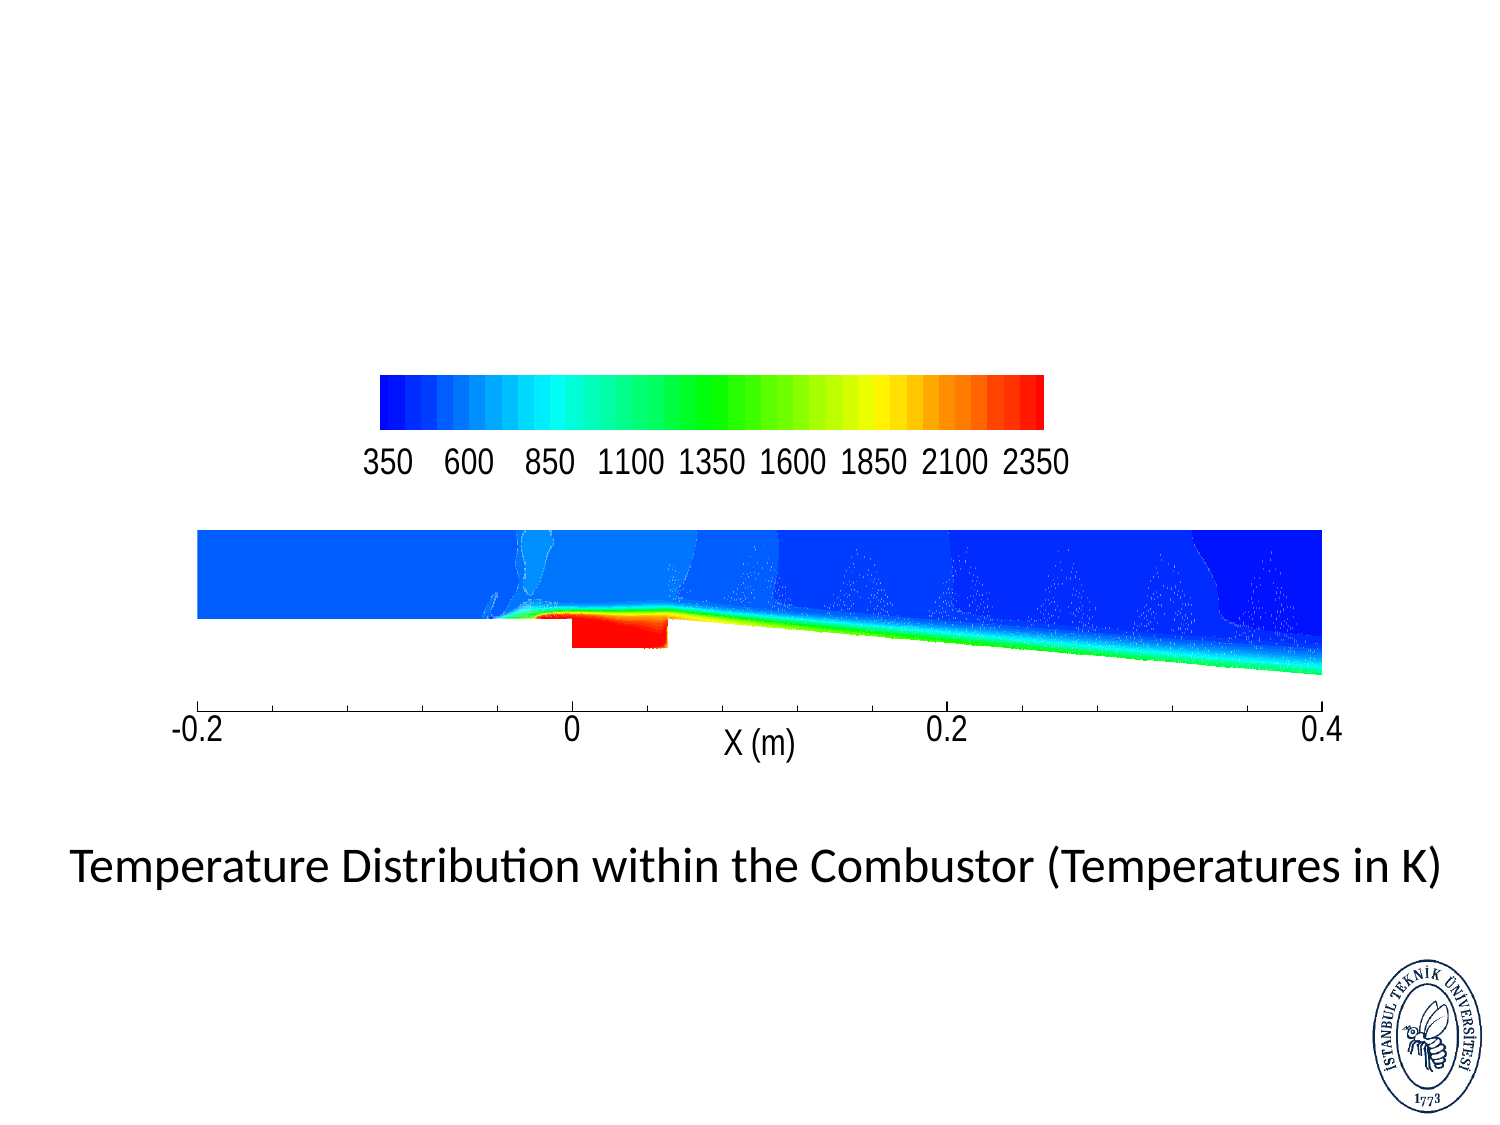
\includegraphics[width=0.95\linewidth,trim=10 40 10 40,clip]{slide106.png}
  \end{center}
  \begin{center}\footnotesize Temperatures in K.\end{center}
\end{frame}

% =========================================================================
% Slide 107 -- OH distribution
% =========================================================================
\begin{frame}{Hydroxyl Radical Distribution within the Cavity}
  \begin{center}
    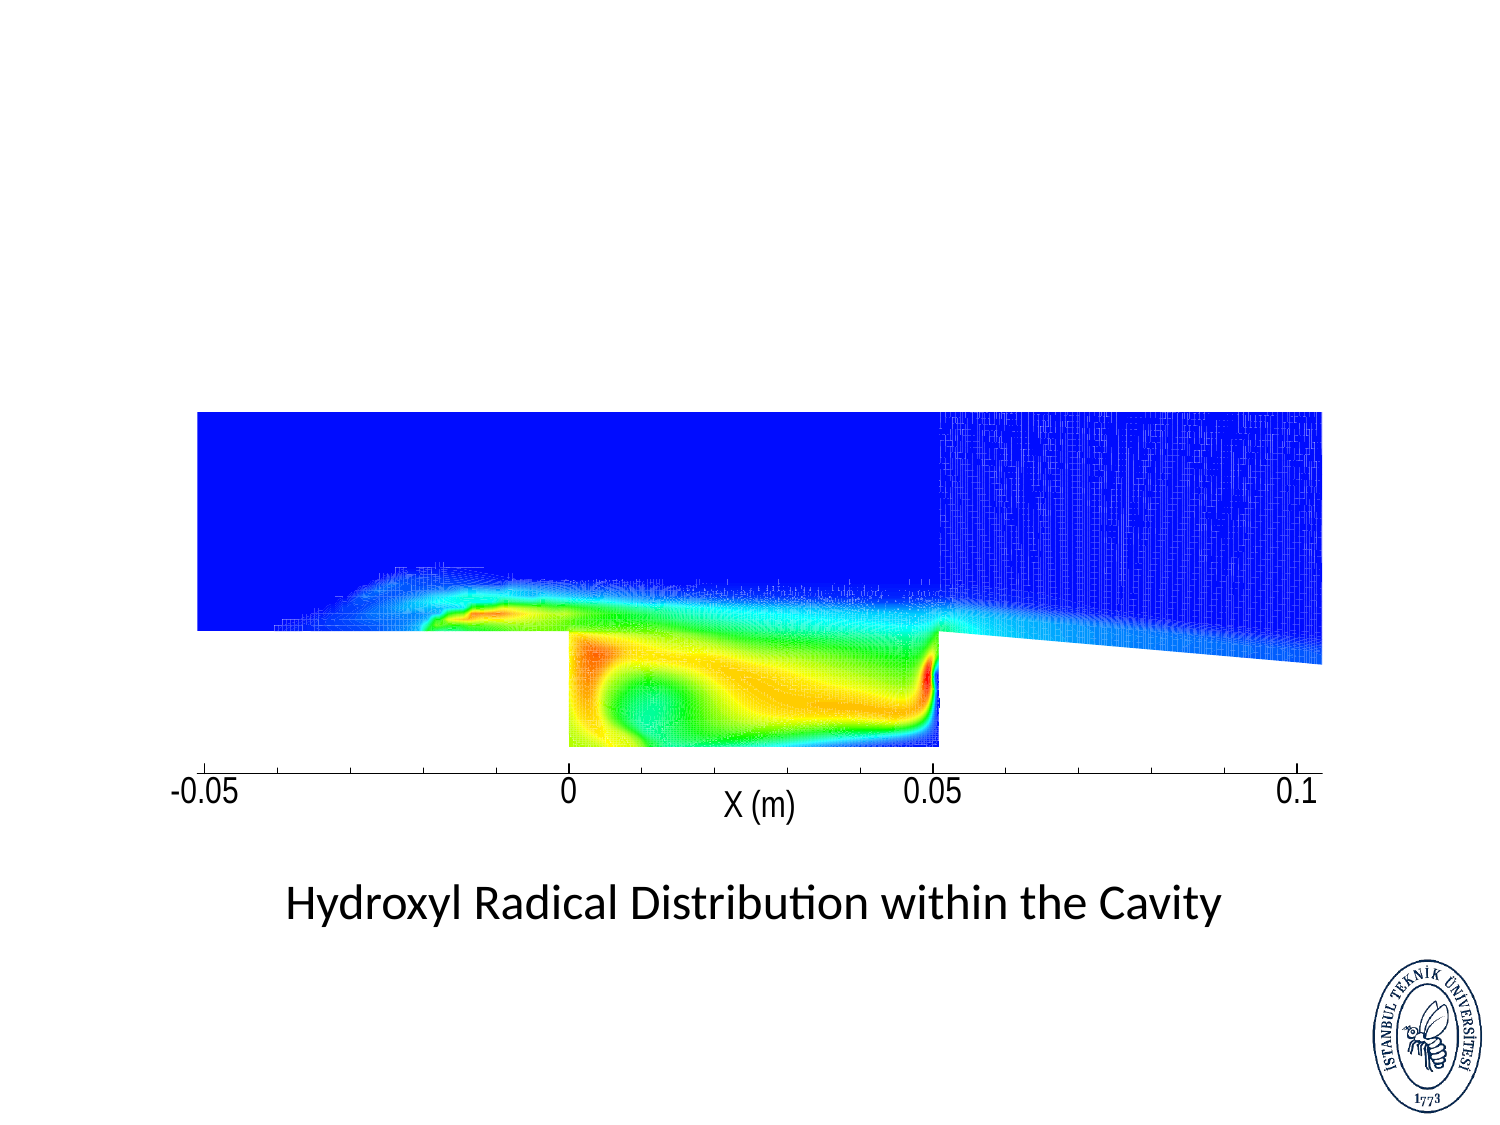
\includegraphics[width=0.95\linewidth,trim=10 40 10 40,clip]{slide107.png}
  \end{center}
\end{frame}

% =========================================================================
% Slide 108 -- Velocity field
% =========================================================================
\begin{frame}{Velocity Field within the Cavity Region}
  \begin{center}
    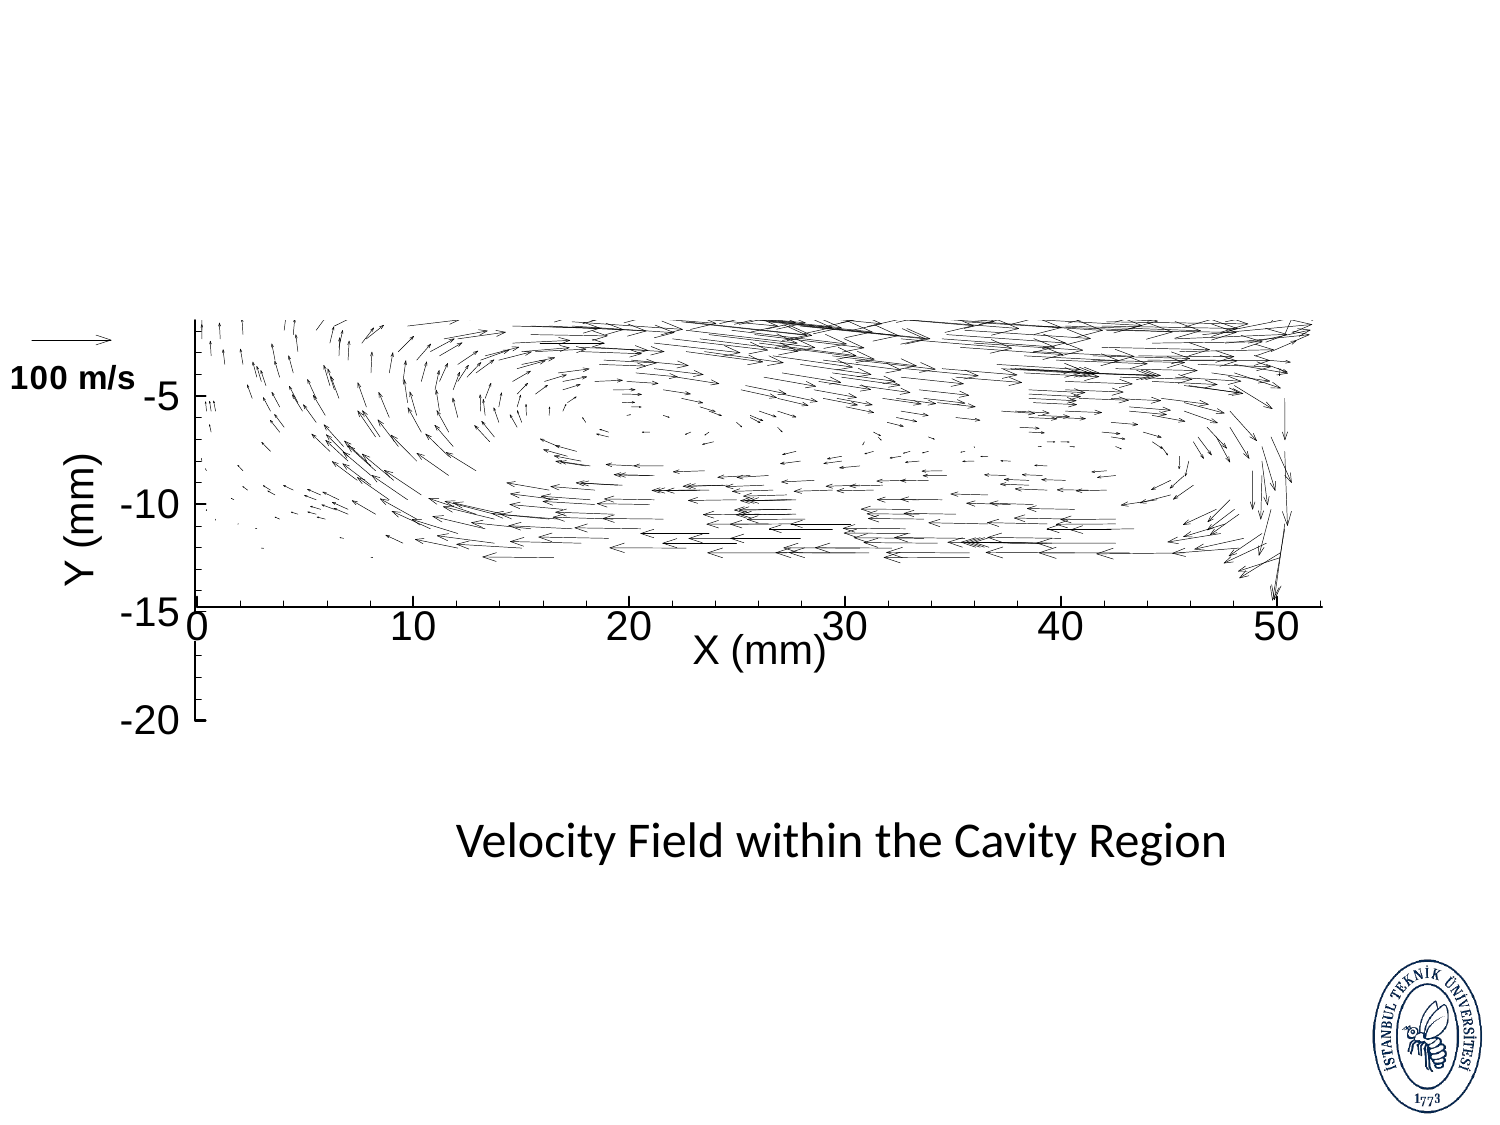
\includegraphics[width=0.85\linewidth,trim=10 40 10 40,clip]{slide108.png}
  \end{center}
\end{frame}

% =========================================================================
% Slide 109 -- Streamlines
% =========================================================================
\begin{frame}{Flow Streamlines within the Cavity}
  \begin{center}
    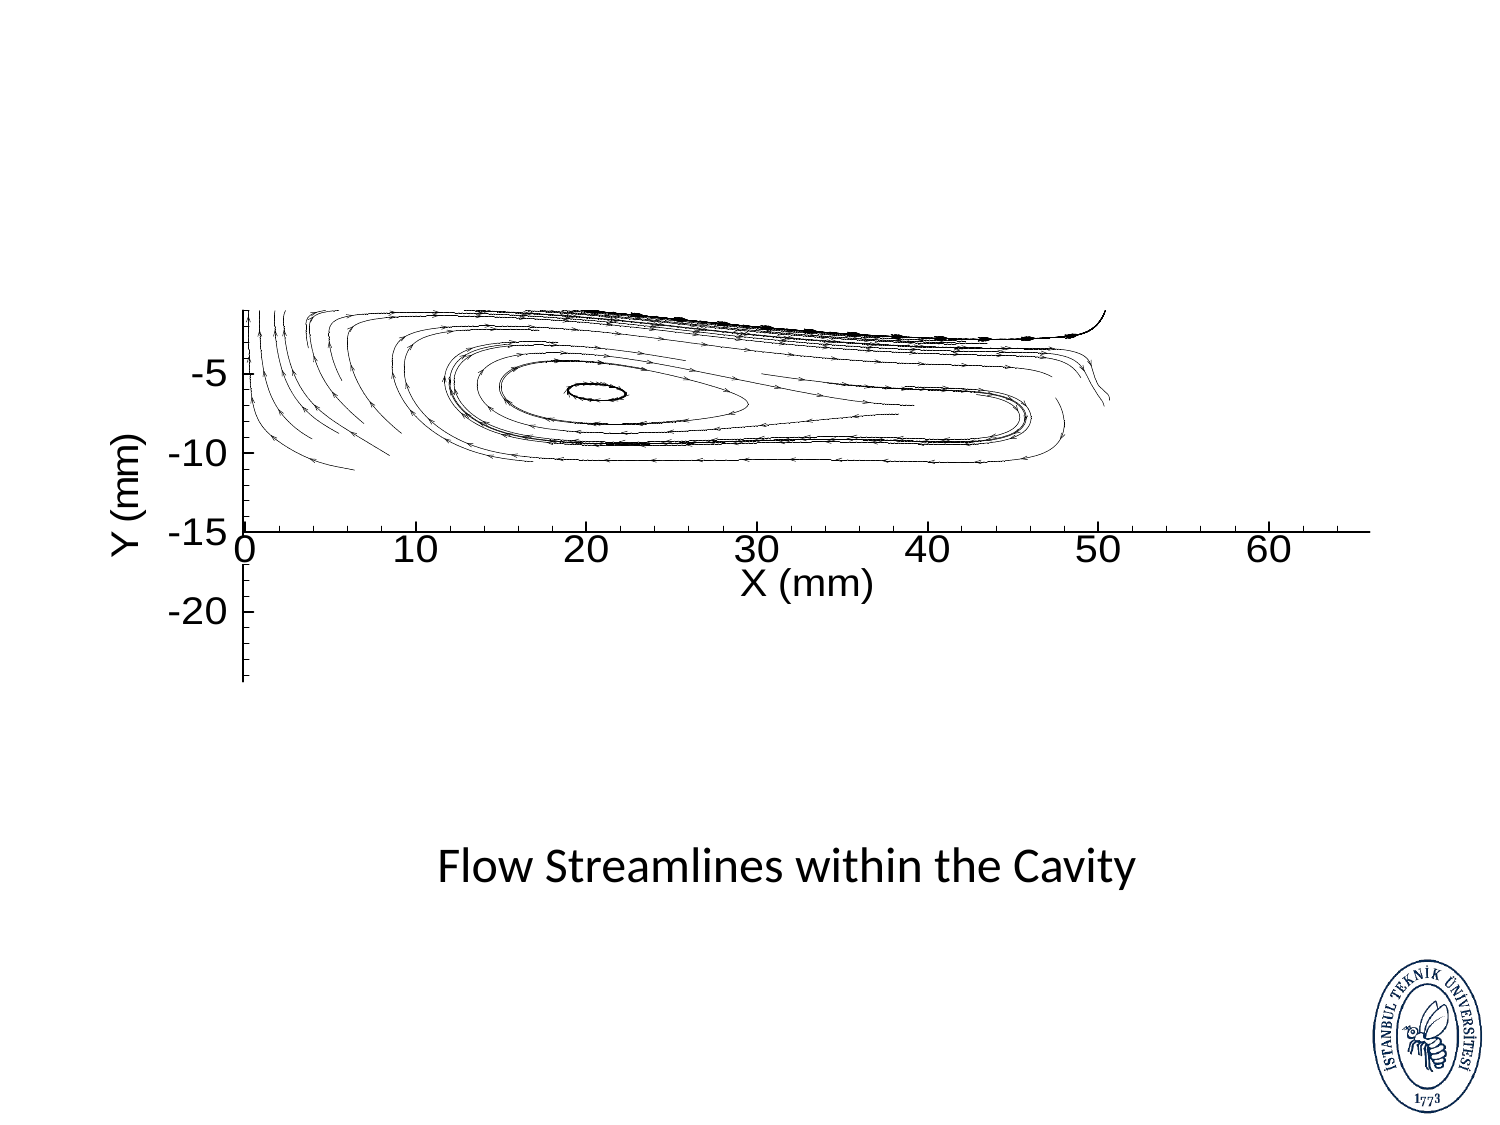
\includegraphics[width=0.85\linewidth,trim=10 40 10 40,clip]{slide109.png}
  \end{center}
\end{frame}

% =========================================================================
% Slide 110 -- Axial velocity along cavity
% =========================================================================
\begin{frame}{Axial Velocity Distribution Along the Length of the Cavity}
  \begin{center}
    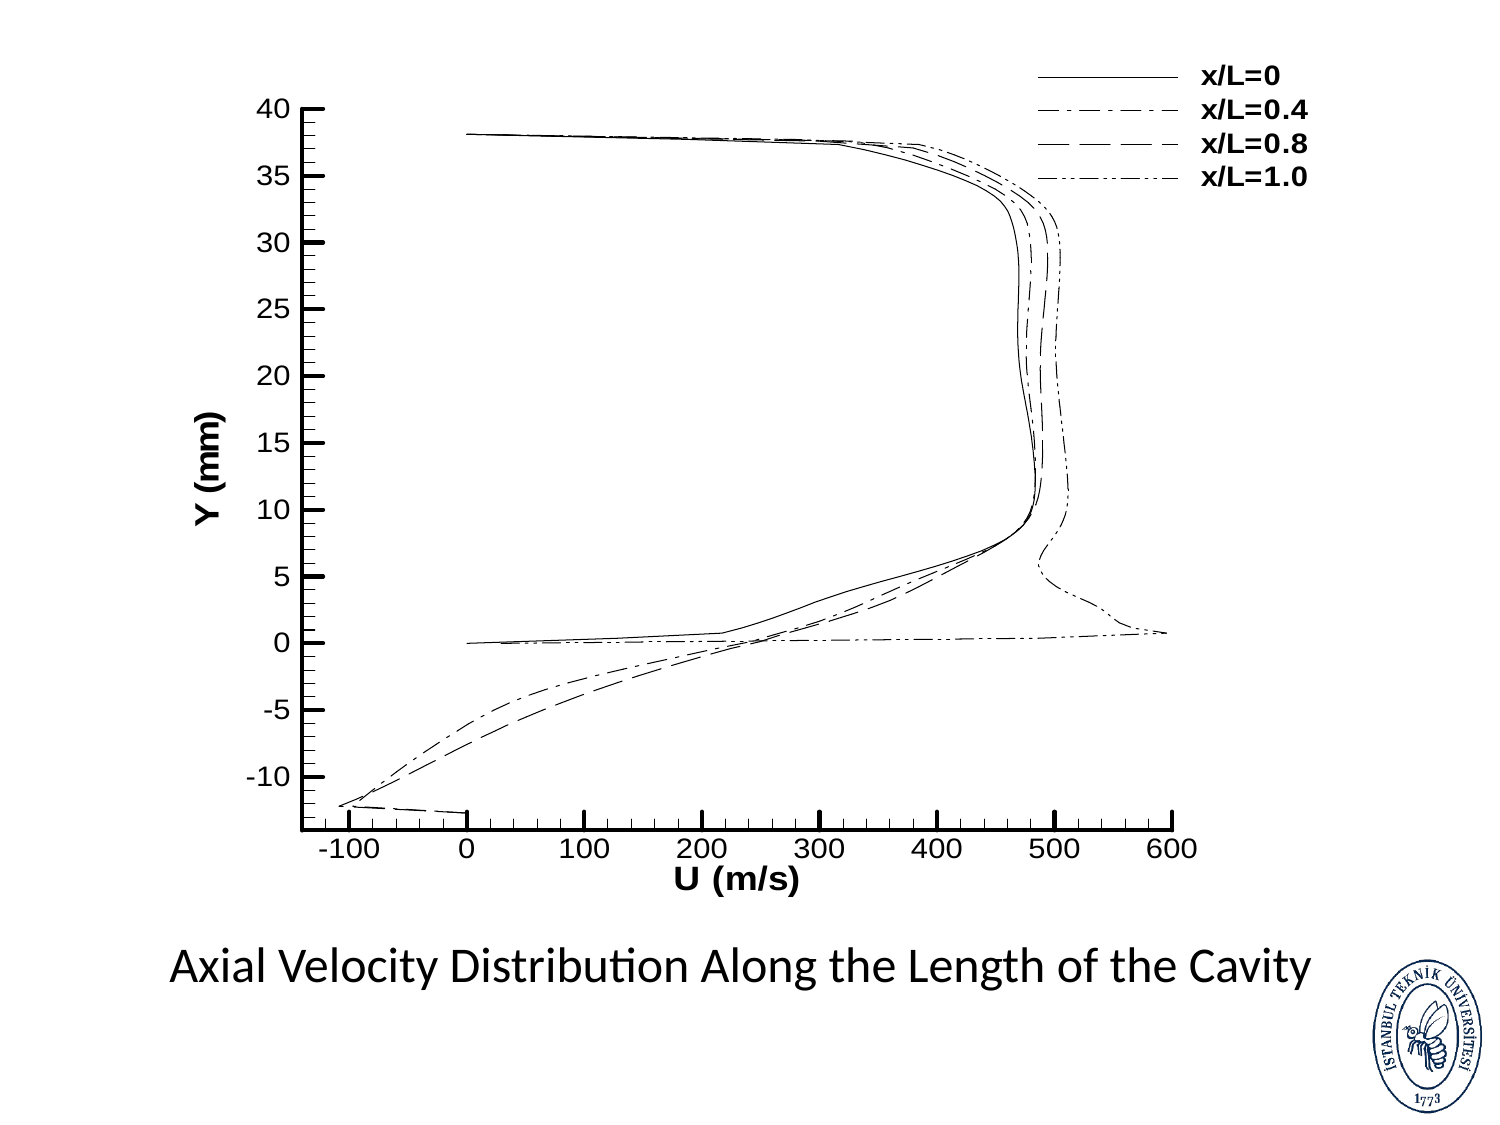
\includegraphics[width=0.78\linewidth,trim=10 40 10 40,clip]{slide110.png}
  \end{center}
\end{frame}

% =========================================================================
% Slide 111 -- Conclusions
% =========================================================================
\begin{frame}{Conclusions}
  \footnotesize
  \begin{itemize}
    \item Flow field and flame-holding mechanism in a ramjet combustor with
          a cavity flame holder have been investigated numerically.
    \item Chemical kinetics are modelled by a multi-step mechanism.
    \item Numerical simulation captures all the essential features of the
          flow field.
    \item Flame anchors at the leading edge of the cavity shear layer and
          spreads into the main flow, consistent with the experiments of
          Micka \& Driscoll (2009).
    \item Reaction zone occupies only a small fraction of the flow field.
    \item Not all the oxygen in the main air stream can participate in
          the reaction.
    \item Excessive thermal loading at the lower wall.
    \item Injection with a pylon could be considered as an alternative.
    \item Further studies are required to design an optimal cavity shape.
    \item Open-source software can be used as an effective design tool.
    \item Parallel computation is necessary to investigate 3-D effects.
  \end{itemize}
\end{frame}

% =========================================================================
% Slide 112 -- Questions
% =========================================================================
\begin{frame}[plain]
  \vfill
  \begin{center}
    {\Huge\bfseries Questions?}
  \end{center}
  \vfill
\end{frame}

\end{document}
